\renewcommand*{\A}{\mathcal{A}}
\newcommand*{\B}{\mathcal{B}}
\renewcommand*{\C}{\mathcal{C}}
\newcommand*{\D}{\mathcal{D}}
\newcommand*{\E}{\mathcal{E}}
\renewcommand*{\L}{\mathcal{L}}
\newcommand*{\R}{\mathcal{R}}
\renewcommand*{\U}{\mathcal{U}}
\newcommand*{\EE}{\mathbb{E}}
\newcommand*{\diag}{\operatorname{diag}}
\renewcommand*{\Re}{\operatorname{Re}}
\renewcommand*{\Im}{\operatorname{Im}}
\newcommand*{\Kern}{\operatorname{Kern}}
\newcommand*{\Eig}{\operatorname{Eig}}
\newcommand*{\iu}{\text{i}}
\newcommand*{\trace}{\operatorname{trace}}
\newcommand*{\rg}{\operatorname{rg}}
\newcommand*{\psd}{\succcurlyeq 0}
\newcommand*{\pd}{\succ 0}
\newcommand*{\nsd}{\preccurlyeq 0}
\newcommand*{\nd}{\prec 0}
\newcommand*{\loc}{{\text{loc}}}
\newcommand*{\GL}{\text{GL}}
\newcommand*{\const}{\text{const}}
\newcommand*{\esssup}{\operatorname{ess\,sup}}
\newcommand*{\Spur}{\operatorname{Spur}}
\newcommand*{\cov}{\operatorname{cov}}
\newcommand*{\opt}{{\text{opt}}}

\newcommand*{\modelscale}{0.85}

\newcommand*{\code}[1]{\texttt{#1}}

\section{%
    Einführung in dynamische Systeme%
}

\subsection{%
    Was ist Kontrolltheorie?%
}

\textbf{Rückführung (feedback)}:
Bei dynamischen Systemen ändern sich die Variablen im Lauf der Zeit, oft durch externe Einflüsse.
Bei einer sog. \begriff{Rückführung (feedback)} sind mehrere dynamische Systeme miteinander
verbunden und beeinflussen sich gegenseitig.

\textbf{Beispiele}:
\begin{itemize}
    \item
    Knopf zur automatischen Geschwindigkeitsreglung in US-amerikanischen Autos

    \item
    Biologie: z.\,B. die Regulierung des Glukosespiegels im Blut, damit dieser konstant bleibt
    (Leber und Pankreas messen bzw. schütten die Hormone Insulin und Glukagon aus und beeinflussen
    sich somit gegenseitig)

    \item
    \begriff{Steuerproblem}: Flug einer Rakete zum Mond mit möglichst wenig Treibstoffaufwand

    \item
    \begriff{Fliehkraftregler (centrifugal governor)}:
    Dieser hält die Rotationsgeschwindigkeit auf einem konstanten Wert,
    der von der Belastung der Maschine unabhängig ist.
    Obwohl er seit dem 17. Jahrhundert bekannt ist, wird er meist Watt/Boulton
    (1788) zugeschrieben.
    Eine theoretische Stabilitätsanalyse wurde von Maxwell und Hurwitz durchgeführt.
    Man spricht von negativer Rückführung, da das Ventil geschlossen/geöffnet wird,
    wenn sich die Maschine zu schnell/zu langsam bewegt.
    Allerdings muss nicht ein stabiles Gleichgewicht eintreten,
    es wäre z.\,B. auch eine Oszillation möglich
    (wie die Temperatur beim Thermostat).
\end{itemize}

\linie

\textbf{positive Auswirkungen von Rückführung}:
\begin{itemize}
    \item
    Erhöhung der Unempfindlichkeit des Systems auf externe Einflüsse\\
    (mehr Glukose durch Essen, Änderung der Belastung beim Fliehkraftregler)

    \item
    Erhöhung der Robustheit gegen Veränderungen in den Komponenten\\
    (Veränderung der Masse des Rades beim Fliehkraftregler)

    \item
    lineares Verhalten bei nicht-linearen Systemen erzwingen\\
    (Autopilot bei Kampfjets, Leistungselektronik)
\end{itemize}

\textbf{negative Auswirkungen von Rückführung}:
\begin{itemize}
    \item
    Erzeugung von dynamischen Instabilitäten, also Oszillationen oder bestimmte Divergenz\\
    (Reduktion der Reibung durch Optimierung der Maschine kann zu Oszillationen beim
    Fliehkraftregler führen)

    \item
    Erhöhung der Empfindlichkeit auf externe Einflüsse und Veränderungen der Komponenten\\
    (Verstärkung des Rauschens bei einem Sensor)
\end{itemize}

\linie

\textbf{Kontrolltheorie}:
Der Zweck von \begriff{Regelung (control)} ist die Gestaltung von Komponenten eines
technischen Rückführungssystems, um ein gewünschtes Gesamtverhalten zu erzielen.\\
\begriff{Kontrolltheorie (control theory)} stellt die notwendigen mathematischen Grundlagen,
Werkzeuge und Algorithmen sowie das nötige Vokabular bzw. die Technik bereit, um dieses Ziel zu
erreichen.

\pagebreak

\subsection{%
    Mathematische Modelle dynamischer Systeme%
}

\textbf{dynamisches System}:\\
In einem \begriff{dynamischen System} treten die Auswirkungen einer Aktion nicht sofort auf.

Zum Beispiel erhöht die Betätigung des Gaspedals im Auto nicht sofort die Geschwindigkeit,
die Temperatur steigt nicht sofort an, wenn die Heizung angeschaltet wird,
Kopfschmerzen verschwinden erst langsam, nachdem Medizin eingenommen wurde, und
eine Geldanlage führt nur in der Zukunft zu Gewinnen oder Verlusten.

Variablen eines dynamischen Systems verändern sich mit der Zeit.
Die Entwicklung hängt dabei von der äußeren Anregung ab, die sich selbst mit der Zeit ändert.

\linie

\textbf{mathematisches Modell}:
Eine Möglichkeit der Analyse des Verhalten eines dynamischen Systems besteht mittels eines
\begriff{mathematischen Modells}.
Solche Modelle werden oft durch (gewöhnliche oder partielle)
\begriff{Dif"|ferentialgleichungen} beschrieben.

\textbf{Beispiel}:
Beim \begriff{gedämpften Federpendel (mass-spring-damper system)} hängt eine Masse $m$ mittels
einer Feder (Federkonstante $k$) an einer Wand (Abstand $q$, abhängig von der Zeit $t$).
Gleichzeitig ist zwischen Masse und Wand eine Dämpfung $c(\dot{q})$ eingebaut, die von der
Geschwindigkeit der Masse abhängt (auch nicht-linear möglich).
Nach dem zweiten Newtonschen Gesetz und dem Hookeschen Gesetz gilt
$m \ddot{q} + c(\dot{q}) + kq = 0$
(Federkraft wirkt in Richtung der Ruheposition).

\linie

\textbf{Eingangsgrößen}:
Ein dynamisches System ist \begriff{autonom (autonomous)},
falls es nicht externen Einflüssen ausgesetzt ist.
Nicht-autonome Systeme haben externe \begriff{Eingangsgrößen (inputs)}.

\textbf{Beispiel}:
Im obigen Beispiel erhält man mit $u(\cdot)$ der externen Kraft, die auf die Masse wirkt,
$m \ddot{q} + c(\dot{q}) + kq = u$.
Die Kraft $u(\cdot)$ variiert normalerweise mit der Zeit.
Je nach Umständen kann sie auf zwei verschiedene Arten interpretiert werden:
\begin{itemize}
    \item
    \begriff{Steuergröße (control input)}:
    falls $u(\cdot)$ frei verändert werden darf

    \item
    \begriff{Störgröße (disturbance input)}:
    falls $u(\cdot)$ durch die Natur feststeht und nicht verändert werden darf
\end{itemize}

\linie

\textbf{Ausgangsgrößen}:
Meistens interessiert man sich nicht für alle Variablen, die in einem Modell vorkommen.
\begriff{Ausgangsgrößen (outputs)} beschreiben die Größen, für die man sich interessiert.

\textbf{Beispiel}:
Wenn man sich im obigen Beispiel nur für die Auslenkung interessiert, dann ist der
Ausgang $y$ bestimmt durch $m \ddot{q} + c(\dot{q}) + kq = u$, $y = q$.
Für eine bestimmte Steuergröße $u(\cdot)$ ist die Ausgangsgröße $y(\cdot)$ eine Funktion in
Abhängigkeit von der Zeit.
Auch $y$ kann auf zwei Arten interpretiert werden:
\begin{itemize}
    \item
    $y$ ist eine Variable, die gemessen werden kann (mittels Sensoren).

    \item
    $y$ ist eine Variable, die zur Analyse der Eigenschaften des Systems überwacht werden soll
    (in der Simulation).
\end{itemize}

\linie
\pagebreak

\textbf{Interpretation des Modells}:
Seien $u(t)$ eine Eingangsgröße, die für $t \ge 0$ definiert ist, und
$q_0$ und $v_0$ eine Anfangsposition bzw. eine Anfangsgeschwindigkeit.
Falls $u \in \C$ und $c \in \C^1$ gilt,
dann hat das Anfangswertproblem $m \ddot{q}(t) + c(\dot{q}(t)) + k q(t) = u(t)$ mit $q(0) = q_0$,
$\dot{q}(0) = v_0$ eine eindeutige, dif"|ferenzierbare Lösung $q(t)$, die für $t \in [0, t_1)$
mit einem $t_1 > 0$ definiert ist
(die Lösung muss nicht für alle $t \ge 0$ existieren).

\textbf{Zustandsgröße}:
Weil die Werte für $q(0)$ und $\dot{q}(0)$ die Lösung der DGL (für eine feste Eingangsgröße)
eindeutig festlegen,
heißen $x = \smallpmatrix{x_1 \\ x_2} := \smallpmatrix{q \\ \dot{q}}$ und
$x(t) = \smallpmatrix{x_1(t) \\ x_2(t)} := \smallpmatrix{q(t) \\ \dot{q}(t)}$
\begriff{Zustandsvektor (state-vector)} bzw. \begriff{Zustandsgröße (state-response)}.
Der \begriff{Ausgang (response)} des Systems ist bestimmt durch $y(t) = q(t)$.

\textbf{Verhalten}:
Bei einem System wie $m \ddot{q} + c(\dot{q}) + kq = u$, $y = q$
ist man an seinem \begriff{Verhalten (behavior)} interessiert,
also die Menge aller Eingangs-, Zustands- und Ausgangsgrößen $u(\cdot)$,
$(q(\cdot), \dot{q}(\cdot))$ und $y(\cdot)$, die diese Gleichung erfüllen.

\textbf{Trajektorien}:
\begriff{Signale (signals)} oder \begriff{Traktorien (trajectories)}
sind vektorwertige Funktionen der Zeit.
Normalerweise wird stillschweigend angenommen, dass sie abschnittsweise stetig sind.

Die Bedingungen, die erfüllt sein müssen, werden oft durch DGLs beschrieben.
Dabei müssen Annahmen gemacht werden, sodass die Existenz und Eindeutigkeit der Lösung des
Anfangswertproblems sichergestellt ist.

\textbf{Äquivalenz}:
Verschiedene Beschreibungen eines Systems können zum selben Verhalten führen.
In diesem Fall heißen die System(-Beschreibungen) \begriff{äquivalent (equivalent)}.
Im sog. \begriff{verhaltens"-basierten Ansatz} bei dynamischen Systemen wird die nötige Theorie in
einer mathematisch präzisen Weise entwickelt.

\linie

\textbf{beispielhafte Fragen}:
\begin{itemize}
    \item
    Falls es keinen externen Einfluss gibt, wie verhalten sich die Zustands- und Ausgangsgröße?

    \item
    Kann das System von einer Position in eine andere gebracht werden
    (\begriff{Steuerproblem, steering problem})?

    \item
    Ist es möglich, die Eingangs- aus der Ausgangsgröße zu rekonstruieren?

    \item
    Kann das System so modifiziert werden, sodass ein gewünschtes Verhalten erzielt wird?
\end{itemize}
Bei manchen von diesen (groben) Fragen muss das System auf seine Eigenschaften hin untersucht
werden, bei anderen müssen Eingangsgrößen verarbeitet oder die Systembedingungen verändert werden,
um das Verhalten des Systems zu ändern.
Mit der Kontrolltheorie versucht man, solche Fragen systematisch zu beantworten.

\linie
\pagebreak

\textbf{von Modellen zweiter zu Modellen erster Ordnung}:
Die Beschreibung $m \ddot{q} + c(\dot{q}) + kq = u$ beinhaltet die ersten beiden
Ableitungen von $q$.
Für $m \not= 0$ heißt sie \begriff{DGL zweiter Ordnung}.
Mit den \begriff{Zustandsvariablen (state-variables)} $x_1 = q$ und $x_2 = \dot{q}$
gilt $\dot{x}_1 = \dot{q} = x_2$, also\\
$\dot{x}_2 = \ddot{q} = -\frac{k}{m} q - \frac{c(\dot{q})}{m} + \frac{1}{m} u
= -\frac{k}{m} x_1 - \frac{1}{m} c(x_2) + \frac{1}{m} u$.
Das kann geschrieben werden als\\
$\dot{x} := \smallpmatrix{\dot{x}_1 \\ \dot{x}_2}
= \smallpmatrix{x_2 \\ -\frac{k}{m} x_1 - \frac{1}{m} c(x_2) + \frac{1}{m} u}
=: f(x, u)$,
man erhält also eine zweidim. \begriff{DGL erster Ordnung}.

\textbf{Lemma (Umwandlung in System erster Ordnung)}:
Sei $r$ eine reellwertige, nicht-lineare Funktion mit $n + 1$ Argumenten.
Dann ist das System
$q^{(n)} + r(q^{(n-1)}, q^{(n-2)}, \dotsc, \dot{q}, q, u) = 0$
äquivalent zu
$\dot{x} := \smallpmatrix{\dot{x}_1 \\ \dot{x}_2 \\ \vdots \\ \dot{x}_{n-1} \\ \dot{x}_n}
= \smallpmatrix{x_2 \\ x_3 \\ \vdots \\ x_n \\ -r(x_n, x_{n-1}, \dotsc, x_2, x_1, u)}
=: f(x, u)$.

Diese Methode ist jedoch nicht eindeutig:

\textbf{Lemma (Umwandlung in System erster Ordnung 2)}:
Sei $r$ eine reellwertige, nicht-lineare Funktion mit $n + 1$ Argumenten.
Dann ist das System
$q^{(n)} + r(q^{(n-1)}, q^{(n-2)}, \dotsc, \dot{q}, q, u) = 0$
äquivalent zu
$\dot{z} := \smallpmatrix{\dot{z}_1 \\ \dot{z}_2 \\ \vdots \\ \dot{z}_{n-1} \\ \dot{z}_n}
= \smallpmatrix{-r(z_1, z_2, \dotsc, z_{n-1}, z_n, u) \\ z_1 \\ \vdots \\ z_{n-2} \\ z_{n-1}}
=: \widehat{f}(z, u)$.

\vspace{3mm}
\linie

\textbf{Zustandsraum-Darstellung}:
Physikalische Modelle führen oft zu einem System von DGLs höherer Ordnung.
Wie gerade gezeigt, können diese oft (aber nicht immer!) äquivalent geschrieben werden als
eine Vektor-DGL erster Ordnung
$\dot{x} = f(x, u)$ und $y = h(x, u)$ mit
Abbildungen $f\colon X \times U \rightarrow \real^n$ und
$h\colon X \times U \rightarrow \real^k$,
wobei $X \subset \real^n$ und $U \subset \real^m$.\\
Ausführlich geschrieben:
\begin{align*}
    \dot{x}_1 &= f_1(x_1, \dotsc, x_n, u_1, \dotsc, u_m),&
    y_1 &= h_1(x_1, \dotsc, x_n, u_1, \dotsc, u_m),\\
    &\;\;\vdots&&\;\;\vdots\\
    \dot{x}_n &= f_n(x_1, \dotsc, x_n, u_1, \dotsc, u_m),&
    y_k &= h_k(x_1, \dotsc, x_n, u_1, \dotsc, u_m).
\end{align*}
Diese Darstellung nennt man die \begriff{Zustandsraum-Darstellung (state-space description)}.
Die Funktionen können auch explizit von der Zeit abhängen.

Wenn $u(\cdot)\colon I \rightarrow U$ eine Eingangsgröße auf einem of"|fenen Intervall
$I \subset \real$ mit $0 \in I$ und $\xi \in \real^n$ eine Anfangsbedingung für den Zustand ist,
dann erhält man die Zustandsgröße durch Lösung des AWP
$\dot{x}(t) = f(x(t), u(t))$, $x(0) = \xi$.
Die Ausgangsgröße ist dann einfach $y(t) := h(x(t), u(t))$ für $t \in I$.

Die Existenz und Eindeutigkeit der Zustandsgröße $x$ auf einem of"|fenen Teilintervall von $I$
ist garantiert, wenn $f$ stetig in $(x, u)$,
$f$ Lipschitz-stetig in $x$ und $u$ stetig ist.
Das gilt auch für Eingänge $u$, die nur abschnittsweise stetig sind (endlich viele Sprungstellen).
In diesem Fall löst man die DGL abschnittsweise und setzt als Anfangsbedingung für
den zweiten Abschnitt den Wert der Lösung im ersten Abschnitt an der Zeit ein, an der
der Sprung stattfindet.
Dadurch ist die Lösung in jedem Fall stetig, wird jedoch Sprünge in der Ableitung besitzen.

\linie

\textbf{allgemeine Beschreibung eines linearen Systems}:
Wenn $f$ und $h$ linear sind, dann gilt
$f(x, u) = Ax + Bu$ und $h(x, u) = Cx + Du$
mit $A \in \real^{n \times n}$, $B \in \real^{n \times m}$, $C \in \real^{k \times n}$,
$D \in \real^{k \times m}$.\\
Daher wird ein allgemeines lineares, zeit-invariantes System,
genannt \begriff{LTI-System (linear, time-\\invariant system)}, beschrieben durch
$\dot{x} = Ax + Bu$, $y = Cx + Du$.

Dieses System wird im Folgenden hauptsächlich verwendet,
denn viele technische Systeme können oft durch lineare Systeme angenähert werden.
Andererseits benötigen physikalische Modelle oft nicht-lineare dynamische Systeme.

\pagebreak

\subsection{%
    \emph{Wiederholung}: Globale Existenz und Eindeutigkeit von Lösungen von Anfangswertproblemen%
}

Sei das Anfangswertproblem $\dot{x} = g(t, x)$, $x(\tau) = \xi$,
für $g\colon D \rightarrow \real^n$ mit $D \subset \real \times \real^n$ gegeben.

\textbf{Voraussetzungen}:
Seien $D \subset \real \times \real^n$ of"|fen und $g\colon D \rightarrow \real^n$
stetig in $(t, x)$ und\\
\begriff{lokal \name{Lipschitz}-stetig} in $x$, d.\,h.
für alle $(\tau, \xi) \in D$ gibt es eine Umgebung $U \subset D$ von $(\tau, \xi)$
und ein $L > 0$ mit
$\norm{g(t, x) - g(t, y)} \le L \norm{x - y}$ für alle $(t, x), (t, y) \in U$.

Die Voraussetzungen sind erfüllt, wenn $g$ und $\partial_x g$ stetig auf $D$ sind,
also insbesondere, wenn $g \in \C^1(D, \real^n)$.

\linie

\textbf{Satz (globale Existenz und Eindeutigkeit)}:
Unter obigen Voraussetzungen gibt es für jedes $(\tau, \xi) \in D$ ein
maximales Existenzintervall $I_{(\tau, \xi)} = (t_-, t_+)$ mit $\tau \in I_{(\tau, \xi)}$
und eine eindeutige $\C^1$-Lösung
$x(\cdot, \tau, \xi)\colon I_{(\tau, \xi)} \rightarrow \real^n$
des AWP $\dot{x} = g(t, x)$, $x(\tau) = \xi$.\\
Maximalität von $I_{(\tau, \xi)}$ bedeutet, dass für jede $\C^1$-Lösung
$x_J\colon J \rightarrow \real^n$ des AWP auf einem Intervall $J$ mit $\tau \in J$
automatisch $J \subset I_{(\tau, \xi)}$ und $x_J = x|_J$ erfüllt ist.\\
Außerdem gilt für $t_+ < \infty$ genau eine der folgenden beiden Eigenschaften
(analog für $t_- > -\infty$):
\begin{itemize}
    \item
    Die Lösung divergiert bestimmt in der Norm:\\
    $\lim_{t \to t_+-0} \norm{x(t)} = \infty$.

    \item
    Die Lösung nähert sich dem Rand von $D$ an:\\
    Für alle Folgen $(t_\nu)_{\nu \in \natural}$ in $I_{(\tau, \xi)}$ mit
    $t_\nu \to t_+$ und $x(t_\nu) \to x_+$
    gilt $(t_+, x_+) \in \partial D$.
\end{itemize}

\pagebreak

\subsection{%
    Simulation%
}

\textbf{Integraldarstellung von DGLs}:
Die Beschreibung eines Systems mit Dif"|ferential- und Ausgangsgleichung
$\dot{x}(t) = f(x(t), u(t))$, $x(0) = \xi$, und $y(t) = h(x(t), u(t))$
erlaubt die numerische Berechnung des Ausgangs (für einen Eingang und eine Anfangsbedingung)
durch ODE-Löser wie z.\,B. \code{ode45} oder \code{ode15s} in MATLAB.
Durch Integration der DGL über die Zeit erhält man die Integraldarstellung
$x(t) = \xi + \int_0^t f(x(\tau), u(\tau))\d\tau$, $y(t) = h(x(t), u(t))$.

Die Darstellung kann man wie folgt interpretieren:
Definiere zunächst die Abbildung $\Sigma_1$ mit
$\smallpmatrix{x(\cdot) \\ u(\cdot)} \mapsto z(\cdot)$,
wobei $z(t) := f(x(t), u(t))$ (\begriff{statisches System (static system)}).
Definiere dann die Integration mit Anfangswert $\xi$:
$\Sigma_2$ mit $v(\cdot) \mapsto w(\cdot)$, wobei $w(t) := \xi + \int_0^t v(\tau)\d\tau$.
Durch Komposition der beiden Abbildungen erhält man die Abbildung $\Sigma_2 \circ \Sigma_1$ mit
$\smallpmatrix{x(\cdot) \\ u(\cdot)} \mapsto w(\cdot)$, wobei
$w(t) := \xi + \int_0^t f(x(\tau), u(\tau))\d\tau$.
Für ein festes $u(\cdot)$ ist nun ein Fixpunkt $x(\cdot)$ dieser Abbildung gesucht.
Dies kann man in einem \begriff{Simulink-Diagramm} darstellen:
\begin{center}
    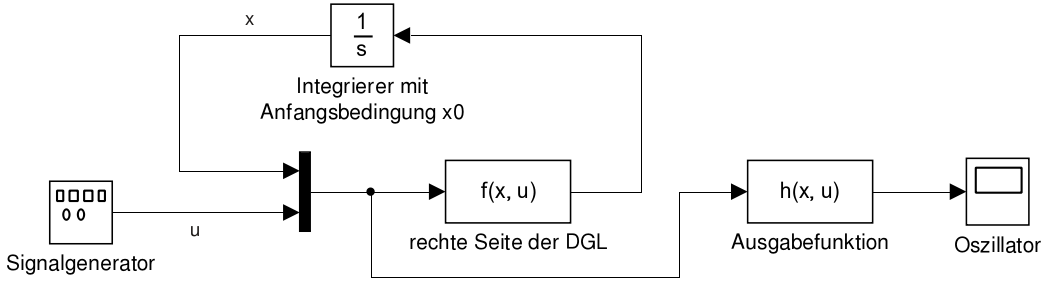
\includegraphics[scale=\modelscale]{dgl}
\end{center}
Den Ausgang erhält man dann einfach durch Anwendung von $h(\cdot, \cdot)$ auf
$x(\cdot)$ und $u(\cdot)$ (wie bei $\Sigma_1$).

\linie

\textbf{inverses Pendel}:
Ein \begriff{inverses Pendel (cart-pendulum system)} ist ein mathematisches Pendel,
das in der Ruhelage nach oben zeigt.
Das Pendel kann nur in einer Dimension schwingen und ist auf einem Wagen befestigt,
der sich in derselben Dimension hin- und her bewegen kann.
Der "`Wagen"' ist so gebaut, dass das Pendel auch nach unten schwingen kann,
es kann also die \SI{360}{\degree} voll ausnutzen.
Das Ziel ist, das Pendel durch Bewegung des Wagens in seiner instabilen Ruhelage zu halten.
Ein Segway kann vereinfacht als inverses Pendel betrachtet werden.

Bezeichnet man
die Masse am Pendel mit $m$,
die Masse des Wagens mit $M$,
die zurückgelegte Strecke des Wagens mit $p$,
die auf den Wagen wirkende Kraft mit $F$,
die Länge des Pendels mit $\ell$ und
den Winkel der Auslenkung des Pendels aus der Ruhelage mit $\theta$,
so erhält man mit den \begriff{\name{Lagrange}-Gleichungen}
$(M + m)\ddot{p} - m\ell \cos(\theta)\ddot{\theta} + c\dot{p} +
m\ell \sin(\theta)\dot{\theta}^2 = F$ sowie\\
$-m\ell \cos(\theta)\ddot{p} + m\ell^2\ddot{\theta} + \gamma \dot{\theta} -
mg\ell \sin(\theta) = 0$,
wobei $c$ und $\gamma$ den Reibungswiderstand des Wagens und des Pendels beschreiben.

Mit $U(\theta) := \smallpmatrix{M + m&-m\ell\cos(\theta)\\-m\ell\cos(\theta)&m\ell^2}$ und
$v(\theta, \dot{p}, \dot{\theta}) := \smallpmatrix{c\dot{p} + m\ell\sin(\theta)\dot{\theta}^2 \\
\gamma\dot{\theta} - mg\ell\sin(\theta)}$
kann man das System schreiben als $U(\theta) \smallpmatrix{\ddot{p} \\ \ddot{\theta}} +
v(\theta, \dot{p}, \dot{\theta}) = \smallpmatrix{F \\ 0}$.
Dabei ist $U(\theta)$ invertierbar, weil die Determinante für kein $\theta$ verschwindet.
Deswegen kann man dies schreiben als\\
$\smallpmatrix{\ddot{p} \\ \ddot{\theta}} = -U(\theta)^{-1} v(\theta, \dot{p}, \dot{\theta}) +
U(\theta)^{-1} \smallpmatrix{F \\ 0} =: \smallpmatrix{w_1(p, \theta, \dot{p}, \dot{\theta}, F) \\
w_2(p, \theta, \dot{p}, \dot{\theta}, F)}$.

Wenn man die Zustandsgrößen $\smallpmatrix{x_1 \\ x_2} := \smallpmatrix{p \\ \theta}$ und
$\smallpmatrix{x_3 \\ x_4} := \smallpmatrix{\dot{p} \\ \dot{\theta}}$
sowie die Eingangsgröße $u := F$ definiert,
so kann das System durch $\dot{x} = f(x, u)$ als System erster Ordnung beschrieben werden,
wobei $f(x, u) := \smallpmatrix{x_3 \\ x_4 \\ w_1(x, u) \\ w_2(x, u)}$.

\pagebreak

\subsection{%
    Gleichgewichte und Linearisierung%
}

\textbf{Gleichgewicht}:
Alle Paare von Vektoren $(x_e, u_e) \in X \times U$ mit $f(x_e, u_e) = 0$ heißen\\
\begriff{Gleichgewichte (equilibria)} des Systems $\dot{x} = f(x, u)$.

%Wenn ein System mit der konstanten Steuergröße $u(t) = u_e$ betrieben und
%der Zustand durch $x_e(t_0) = x_e$ initialisiert wird, so gilt für die Zustandsgröße
%$x(t) = x_e$ und $\dot{x}(t) = 0$ für alle $t \ge t_0$,
%d.\,h. wenn ein System im Gleichgewicht startet,
%dann bleibt die Zustandsgröße auch da.

Wenn ein System mit der konstanten Steuergröße $u(t) = u_e$ betrieben wird,
der Zustand durch $x_e(t_0) = x_e$ initialisiert wird und die Lösung des Systems eindeutig ist,
dann gilt $x(t) \equiv x_e$ für alle $t \ge t_0$
(weil das eine Lösung ist, da $f(x_e, u_e) = 0$).

\textbf{Beispiel}:
Für Gleichgewichte in obiger DGL müssen die Ableitungen von $p$ und $\theta$ verschwinden,
also $0 = F$ und $-mg\ell \sin(\theta) = 0$.
Die Lösungen sind $\theta_e = 0$ (aufrechte Position) und $\theta_e = \pi$ (nach unten zeigend),
wobei $p_e$ beliebig ist.

\linie

\textbf{Herleitung der Linearisierung}:
Falls $f$ und $h$ stetig dif"|ferenzierbar sind, kann man die Taylorentwicklungen erster Ordnung
um $(x_e, u_e)$ berechnen als\\
$f(x, u) \approx f(x_e, u_e) + \partial_x f(x_e, u_e) (x - x_e) +
\partial_u f(x_e, u_e) (u - u_e)$ und\\
$h(x, u) \approx y_e + \partial_x h(x_e, u_e) (x - x_e) +
\partial_u h(x_e, u_e) (u - u_e)$, wobei $y_e := h(x_e, u_e)$.\\
Dabei sind die partiellen Ableitungen die Jacobi-Matrizen.
Die Näherung ist besonders gut, falls $x \approx x_e$ und $u \approx u_e$.
Daher kann man die Entwicklungen zur Linearisierung von nicht-linearen Systemen verwenden.

\textbf{Linearisierung}:
Seien $f(x_e, u_e) = 0$ und $f, h \in \C^1$.
Dann ist die \begriff{Linearisierung (linearization)} von $\dot{x} = f(x, u)$, $y = h(x, u)$
bei $(x_e, u_e)$ gegeben durch
$\dot{x}_\Delta = A x_\Delta + B u_\Delta$, $y_\Delta = C x_\Delta, + D u_\Delta$,
wobei $A := \partial_x f(x_e, u_e)$, $B := \partial_u f(x_e, u_e)$,
$C := \partial_x h(x_e, u_e)$, $D := \partial_u h(x_e, u_e)$.

Für die betrachteten $t$ gelte $u(t) \approx u_e$ und $x(t) \approx x_e$.
Für die nicht-lineare Ausgangsgröße gilt also $y(t) \approx y_e$.
Wenn man nun die Linearisierung mit $u_\Delta := u(t) - u_e$ für den Anfangswert
$x_\Delta(0) := x(0) - x_e$ ausführt, so hofft man, dass
$y_e + y_\Delta(t)$ die nicht-lineare Ausgangsgröße $y(t)$ gut approximiert.\\
Es gilt nämlich $\left[x(t) - x_e\right]^\cdot = \dot{x}(t) = f(x(t), u(t)) \approx
A[x(t) - x_e] + Bu_\Delta(t)$ nach Definition der Linearisierung
($(x_e, u_e)$ ist nämlich ein Gleichgewicht).
Wenn die Trajektorie $x(\cdot)$ nahe an $x_e$ bleibt, dann ist die Taylor-Abschätzung
besonders gut -- würde ein Gleichheitszeichen stehen, dann wäre $[x(t) - x_e]$
ebenfalls eine Lösung der Linearisierung, es müsste also $x_\Delta(t) = x(t) - x_e$ gelten.
Aufgrund der nur ungefähren Gleichheit gilt aber nur $x_\Delta(t) \approx x(t) - x_e$.\\
Außerdem gilt $\left[y(t) - y_e\right] = h(x(t), u(t)) - y_e \approx C[x(t) - x_e] + Du_\Delta(t)$.
Für $x_\Delta(t) \approx x(t) - x_e$ ist die rechte Seite ungefähr gleich $y_\Delta(t)$,
also $y_\Delta(t) \approx y(t) - y_e$.
So erhält man $y(t) \approx y_e + y_\Delta(t)$.

\linie

\textbf{Beispiel}:
Man betrachtet das inverse Pendel im nach unten zeigenden, stabilen Gleichgewicht.
Wenn man nur kurz eine Kraft anwendet, dann schlägt das Pendel nur kurz in beide Richtungen
aus, ehe es sich wieder im Gleichgewicht befindet.
Weil keine großen Abweichungen der Position auftreten, ist die zugehörige Linearisierung eine
ziemlich gute Annäherung.\\
Anders sieht es aus, wenn man das Pendel im oberen, instabilen Gleichgewicht startet
und dieselbe Kraft kurz anwendet.
Dann wird das Pendel nach unten schwingen und sich im unteren Gleichgewicht einpendeln.
Wegen der großen Abweichungen der Position zur Startposition ist die Linearisierung für
das obere Gleichgewicht keine gute Annäherung.

\pagebreak

\subsection{%
    Systemverbindungen und Blockdiagramme%
}

\begriff{Modularität} ist eines der wichtigsten Konzepte bei der Modellierung von
dynamischen Systemen.
Komplexe Modelle werden durch Verbindung einfacher Systemkomponenten in einer Art Hierarchie
verbunden.
Die \begriff{Verbindung} geschieht dabei durch Gleichsetzung von Signalen.

\textbf{Vorteile der Modularität}:
\begin{itemize}
    \item
    Benutzung von Softwarebibliotheken mit Standard-Systemkomponenten und
    Schnittstellen zwischen verschiedenen physikalischen Bereichen

    \item
    Benutzung von Modellierungspaketen (MATLAB, Modelica)

    \item
    Übersichtlichkeit auch bei komplexen Modellen durch die hierarchische, verschachtelte
    Struktur

    \item
    Veränderung von einzelnen Komponenten, ohne das Gesamtgefüge zu zerstören
\end{itemize}

\linie

\textbf{Beispiel}:
Beim inversen Pendel geht man davon aus, dass die Kraft des Wagens durch einen
elektrischen Gleichstrom-Motor an einem Rad mit Radius $r$ erzeugt wird.
Wenn die Spannung $V$ an den Motor angelegt wird, dann erzeugt der Strom in den Spulen
ein Drehmoment.
Wenn $T$ das Lastmoment des Motors ist, dann wird die Dynamik des Motors durch
$J\ddot{\phi} + b\dot{\phi} = k_m I - T$, $L\dot{I} + RI = V - k_e\dot{\phi}$
beschrieben, wobei $J, b, k_m, L, R, k_e > 0$ konstant sind.
Man nimmt an, dass das Lastmoment und der Winkel der Motorwelle durch
$T = Fr$ und $p = r\phi$ mit $F$ und $p$ zusammenhängen.
Diese Gleichungen muss man nun mit der ursprünglichen DGL des inversen Pendels kombinieren.
Man erhält dann
$L\dot{I} + RI + \frac{k_e}{r}\dot{p} = V$,\\
$\left(M + m + \frac{J}{r^2}\right)\ddot{p} - m\ell \cos(\theta)\ddot{\theta} +
\left(c + \frac{b}{r^2}\right)\dot{p} + m\ell \sin(\theta)\dot{\theta}^2 -
\frac{k_m}{r}I = 0$ sowie\\
$-m\ell \cos(\theta)\ddot{p} + m\ell^2\ddot{\theta} + \gamma \dot{\theta} -
mg\ell \sin(\theta) = 0$.\\
Die gekoppelten Gleichungen heißen oft auch \begriff{beidseitig gekoppelt},
weil sich die Dynamik beider Systeme gegenseitig beeinflusst.
Für $k_e = 0$ wäre die Kopplung \begriff{einseitig}
(die erste Gleichung könnte dann separat gelöst werden).\\
In der Simulation erkennt man, dass für kleines $L$ (Motor kann die Kraft schnell aufwenden)
die Lösung sich kaum von der Lösung ohne Motor unterscheidet.
Für größeres $L$ (nur langsame Aufwendung der Kraft) unterscheiden sich
die beiden Systeme jedoch erheblich.

\linie

\textbf{Reihenschaltung}:
Die \begriff{Reihenschaltung (series interconnection)} der Systeme\\
$\dot{x}_1 = f_1(x_1, u_1)$, $y_1 = h_1(x_1, u_1)$ und
$\dot{x}_2 = f_2(x_2, u_2)$, $y_2 = h_2(x_2, u_2)$
erhält man, wenn man den Ausgang des ersten Systems mit dem Eingang des zweiten Systems
verbindet, also $u_2 = y_1$
(dabei müssen die Dimensionen übereinstimmen).
Man erhält das System\\
$\dot{x} = f(x, u_1)$, $y_2 = h_2(x_2, h_1(x_1, u_1))$,
wobei $x := \smallpmatrix{x_1 \\ x_2}$ und
$f(x, u_1) := \smallpmatrix{f_1(x_1, u_1) \\ f_2(x_2, h_1(x_1, u_1))}$.

Für lineare Systeme
$\dot{x}_1 = A_1 x_1 + B_1 u_1$, $y_1 = C_1 x_1 + D_1 u_1$ und\\
$\dot{x}_2 = A_2 x_2 + B_2 u_2$, $y_2 = C_2 x_2 + D_2 u_2$ entspricht dies
$\dot{x} = Ax + Bu_1$, $y_2 = Cx + Du_1$\\
mit $x := \smallpmatrix{x_1 \\ x_2}$ sowie
$A := \smallpmatrix{A_1 & 0 \\ B_2 C_1 & A_2}$,
$B := \smallpmatrix{B_1 \\ B_2 D_1}$,
$C := \smallpmatrix{D_2 C_1 & C_2}$ und
$D := D_2 D_1$.

\linie

\textbf{Parallelschaltung}:
Die \begriff{Parallelschaltung (parallel interconnection)} der Systeme\\
$\dot{x}_1 = f_1(x_1, u_1)$, $y_1 = h_1(x_1, u_1)$ und
$\dot{x}_2 = f_2(x_2, u_2)$, $y_2 = h_2(x_2, u_2)$
erhält man, wenn beide denselben Eingang haben und man die Ausgänge summiert,
also $u_1 = u_2 = u$ und $y = y_1 + y_2$
(dabei müssen die Dimensionen übereinstimmen).
Man erhält das System\\
$\dot{x} = f(x, u)$, $y = h_1(x_1, u) + h_2(x_2, u)$,
wobei $x := \smallpmatrix{x_1 \\ x_2}$ und
$f(x, u) := \smallpmatrix{f_1(x_1, u) \\ f_2(x_2, u)}$.

Für lineare Systeme
$\dot{x}_1 = A_1 x_1 + B_1 u_1$, $y_1 = C_1 x_1 + D_1 u_1$ und\\
$\dot{x}_2 = A_2 x_2 + B_2 u_2$, $y_2 = C_2 x_2 + D_2 u_2$ entspricht dies
$\dot{x} = Ax + Bu$, $y = Cx + Du$\\
mit $x := \smallpmatrix{x_1 \\ x_2}$ sowie
$A := \smallpmatrix{A_1 & 0 \\ 0 & A_2}$,
$B := \smallpmatrix{B_1 \\ B_2}$,
$C := \smallpmatrix{C_1 & C_2}$ und
$D := D_1 + D_2$.

\linie
\pagebreak

\textbf{Control System Toolbox}:
Die \begriff{Control System Toolbox} von MATLAB stellt sog. \begriff{\code{ss}-Objekte} bereit,
die lineare Systeme darstellen.
Die Verwendung erfolgt wie folgt:
\begin{itemize}
    \item
    Definition: \code{sys = ss(A, B, C, D)}

    \item
    Reihenschaltung: \code{sys = sys1 * sys2}

    \item
    Parallelschaltung: \code{sys = sys1 + sys2}

    \item
    Simulation: \code{y = lsim(sys, u, T, x0)}

    \item
    Bestimmung der definierenden Matrizen: \code{[A, B, C, D] = ssdata(sys)}
\end{itemize}
Die überladenen Operatoren \code{*} und \code{+} erinnern an die zugehörigen Operationen
der Matrizen, die bei der Bildung der Reihen- bzw. Parallelschaltung verwendet werden.

\linie

\textbf{Blockdiagramm}:
Ein \begriff{Blockdiagramm (block-diagram)} besteht aus Verbindungen von einzelnen Blöcken.
Solche Diagramme sollten bestimmten algebraischen Gleichungen entsprechen.

\textbf{Beispiele}:
\begin{itemize}
    \item
    \textbf{Reihenschaltung}:\\
    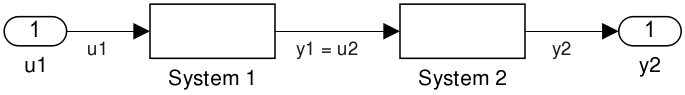
\includegraphics[scale=\modelscale]{schaltung_reihe.png}

    \item
    \textbf{Parallelschaltung}:\\
    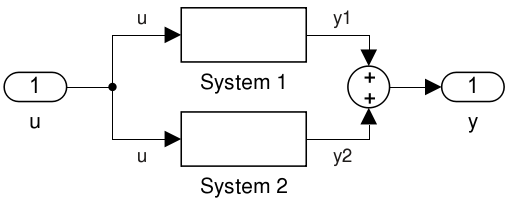
\includegraphics[scale=\modelscale]{schaltung_parallel.png}

    \item
    \textbf{gedämpftes Federpendel}:\\
    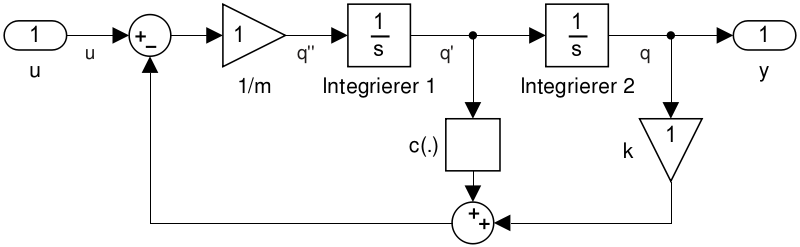
\includegraphics[scale=\modelscale]{federpendel_gedaempft.png}

    \item
    \textbf{allgemeines lineares System}:
    (in Simulink auch darstellbar durch einen \code{State-Space}- oder \code{LTI Systems}-Block,
    definiert durch $A, B, C, D$ bzw. ein \code{ss}-Objekt)\\
    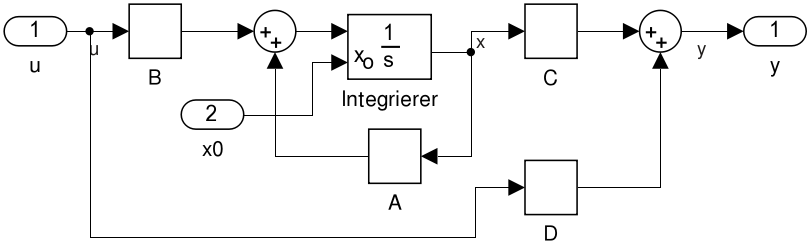
\includegraphics[scale=\modelscale]{lineares_system.png}
\end{itemize}

\pagebreak

\chapter{%
    Lösungen von linearen Systemen%
}

\section{%
    Diagonalisierbare Matrizen%
}

Die Zustandsraum-Darstellung eines dynamischen Systems ohne Ein- und Ausgang ist
$\dot{x} = f(x)$ mit $f\colon X \rightarrow \real^n$, $X \subset \real^n$.
Das System ist linear, falls $f$ eine lineare Abbildung ist.
Daher wird ein lineares, autonomes System beschrieben durch $\dot{x} = Ax$ mit
$A \in \real^{n \times n}$.
Lösungen solcher Systeme sind durch Methoden der linearen Algebra vollständig bekannt.

\linie

\textbf{diagonale Matrix}:
Für $A = \diag(\lambda_1, \dotsc, \lambda_n)$ mit $\lambda_k \in \real$, $k = 1, \dotsc, n$,
ist das System äquivalent zu $\dot{x}_1 = \lambda_1 x_1$, \dots, $\dot{x}_n = \lambda_n x_n$.
Jede Gleichung dieses vollkommen entkoppelten Systems kann separat gelöst werden.
Als Lösungen erhält man $x_k(t) = e^{\lambda_k t} \xi_k$, $\xi_k \in \real$, für
$k = 1, \dotsc, n$.
Kompakter lässt sich das schreiben als
$x(t) = \smallpmatrix{e^{\lambda_1 t} & & 0 \\ & \ddots & \\ 0 & & e^{\lambda_n t}} \xi$ mit
$\xi = \smallpmatrix{\xi_1 \\ \vdots \\ \xi_n}$, wobei $x(0) = \xi$ gilt.

\linie

Für $A$ nicht diagonal muss man eine Koordinatentransformation durchführen.

\textbf{Zustandskoordinaten-Transformation}:
Jede invertierbare Matrix $T \in \real^{n \times n}$ definiert eine
\begriff{Zustandskoordinaten-Transformation (state-coordinate transformation)} $z = Tx$.

Wenn $x(t)$ die Gleichung $\dot{x}(t) = Ax(t)$ erfüllt, dann gilt mit $z(t) := Tx(t)$, dass\\
$\dot{z}(t) = T\dot{x}(t) = TAx(t) = TAT^{-1} Tx(t) = \widetilde{A} z(t)$,
wobei in den neuen Koordinaten das System durch $\widetilde{A} := TAT^{-1}$ beschrieben wird.
Umgekehrt erfüllt $x(t) := T^{-1} z(t)$ die DGL $\dot{x}(t) = Ax(t)$, falls
$z(t)$ die DGL $\widetilde{z}(t) = \widetilde{A} z(t)$ erfüllt.

Die Lösungsmenge von $\dot{z} = \widetilde{A} z$ transformiert sich also linear durch $T^{-1}$
in die Lösungsmenge von $\dot{x} = Ax$.

\linie

Oft ist $A$ zwar nicht diagonal, dafür aber diagonalisierbar.

\textbf{Satz (Lösung von $\dot{x} = Ax$ für $A$ diagonalisierbar)}:\\
Sei $T \in \real^{n \times n}$, sodass
$TAT^{-1} = \diag(\lambda_1, \dotsc, \lambda_n)$
mit $\lambda_1, \dotsc, \lambda_n \in \real$.
Dann ist die eindeutige Lösung von $\dot{x} = Ax$, $x(0) = \xi$, gegeben durch
$x(t) := \left[T^{-1} \diag(e^{\lambda_1 t}, \dotsc, e^{\lambda_n t}) T\right] \xi$.

Jede Komponente einer Lösung $x$ von $\dot{x} = Ax$ ist eine
Linearkombination von $e^{\lambda_k t}$, $k = 1, \dotsc, n$.
Genauer: Wenn $\xi$ gleich einer der Spalten $c_k$ von $S := T^{-1}$ ist,
dann ist $x(t) = c_k e^{\lambda_k t}$,
da
$Se_k = c_k$ und
$S \diag(e^{\lambda_1 t}, \dotsc, e^{\lambda_n t}) (S^{-1} c_k) =
S (\diag(e^{\lambda_1 t}, \dotsc, e^{\lambda_n t}) e_k) = S (e^{\lambda_k t} e_k) =
c_k e^{\lambda_k t}$.\\
Alle anderen Lösungen sind wegen Linearität Linearkombinationen dieser $n$ Lösungen:\\
$[S \diag(e^{\lambda_1 t}, \dotsc, e^{\lambda_n t}) S^{-1}] (\sum_{k=1}^n \mu_k c_k)
= \sum_{k=1}^n \mu_k c_k e^{\lambda_k t}$.

\textbf{Beispiel}:
Beim linearisierten inversen Federpendel bekommt man im oberen Gleichgewicht die Matrix
$A = \smallpmatrix{0 & 0 & 1 & 0 \\ 0 & 0 & 0 & 1 \\
0 & 3.92 & -2 & -0.32 \\ 0 & 22.1 & -3.23 & -1.82}$.
Man erhält Matrizen
$S = \smallpmatrix{1 & -0.03 & -0.04 & 0.58 \\ 0 & -0.26 & -0.16 & -0.11 \\
0 & -0.12 & 0.22 & -0.79 \\ 0 & -0.96 & 0.96 & 0.16}$ und
$\Lambda = \diag(0, 3.72, -6.16, -1.38)$ mit $\Lambda = S^{-1} AS$.
Die Lösung divergiert nicht bestimmt genau dann, wenn
$\xi \in \left\{S \left.\smallpmatrix{\widetilde{\xi}_1 \\ 0 \\
\widetilde{\xi}_3 \\ \widetilde{\xi}_4} \;\right|\;
\widetilde{\xi}_1, \widetilde{\xi}_3, \widetilde{\xi}_4 \in \real\right\}$.

\vspace{3mm}
\linie
\pagebreak

\textbf{komplexe Transformationen und Diagonalmatrizen}:
Für die Linearisierung im unteren Gleichgewicht sind die Matrizen
$T = \smallpmatrix{r_1 \\ r_2 \\ r_3 \\ r_4}$,
$S = \smallpmatrix{c_1 & c_2 & c_3 & c_4}$ und
$\Lambda = \diag(\lambda_1, \lambda_2, \lambda_3, \lambda_4)$ komplex.
Dennoch stimmt obiger Satz, denn Eigenwerte von reellen Matrizen treten immer komplex konjugiert
auf.
Hier ist z.\,B. $\lambda_2 = \overline{\lambda_3}$, $c_2 = \overline{c_3}$ und
$r_2 = \overline{r_3}$.
Daher ist\\
$\left[T^{-1} \diag(e^{\lambda_1 t}, e^{\lambda_2 t}, e^{\lambda_3 t}, e^{\lambda_4 t}) T\right]
= \smallpmatrix{c_1 e^{\lambda_1 t} & c_2 e^{\lambda_2 t} &
\overline{c_2} e^{\overline{\lambda_2} t} & c_4 e^{\lambda_4 t}}
\smallpmatrix{r_1 \\ r_2 \\ \overline{r_2} \\ r_4}$\\
$= e^{\lambda_1 t} c_1 r_1 + e^{\lambda_2 t} c_2 r_2 +
e^{\overline{\lambda_2} t} \overline{c_2} \overline{r_2} + e^{\lambda_4 t} c_4 r_4
= e^{\lambda_1 t} c_1 r_1 + 2 \Re\!\left[e^{\lambda_2 t} c_2 r_2\right] + e^{\lambda_4 t} c_4 r_4$
immer eine reelle Matrix.
Dementsprechend ist die Lösung für den Anfangswert $\xi \in \real^4$ gleich\\
$e^{\lambda_1 t} c_1 (r_1 \xi) + 2 \Re\!\left[e^{\lambda_2 t} c_2 (r_2 \xi)\right] +
e^{\lambda_4 t} c_4 (r_4 \xi)$.

Das lässt sich noch etwas vereinfachen:
Für $\lambda = \sigma + \iu \omega \in \complex$ ($\sigma, \omega \in \real$) gilt\\
$e^{\lambda t} = e^{\sigma t}[\cos(\omega t) + \iu \sin(\omega t)]$.
Wenn also $c$ und $r$ komplexe Spalten- bzw. Zeilenvektoren sind, dann ist
$cr = [\Re(c) + \iu \Im(c)] [\Re(r) + \iu \Im(r)] = M + \iu N$ mit
$M := [\Re(c) \Re(r) - \Im(c) \Im(r)]$ und $N := [\Re(c) \Im(r) + \Im(c) \Re(r)]$.\\
Das führt zur expliziten Formel
$\Re\!\left[e^{\lambda t} c r\right] = e^{\sigma t} [\cos(\omega t) M - \sin(\omega t) N]$.\\
Die Komponenten von $\Re\!\left[e^{\lambda t} c r\right] \xi$ sind also
gleichbleibende ($\sigma = 0$),
wachsende ($\sigma > 0$) oder
kleiner werdende ($\sigma < 0$) Oszillationen.

\linie

Bei der Diagonalisierung einer Matrix $A \in \real^{n \times n}$ bestimmt man für jeden
Eigenwert $\lambda$ eine Basis des zugehörigen Eigenraums $\Kern(A - \lambda I)$.
Die Basen aller Eigenräume fasst man zu $v_1, \dotsc, v_g$ zusammen,
diese Menge ist automatisch linear unabhängig und daher $g \le n$.

\textbf{Satz (Diagonalisierbarkeitskriterium)}:
Seien $v_1, \dotsc, v_g$ linear unabhängige Eigenvektoren zu Eigenwerten
$\lambda_1, \dotsc, \lambda_g$ der Matrix $A \in \real^{n \times n}$,
sodass keine größere Liste linear unabhängiger Eigenvektoren existiert.
Dann ist $A$ diagonalisierbar genau dann, wenn $g = n$.
In diesem Fall ist $S^{-1} A S = \diag(\lambda_1, \dotsc, \lambda_n)$ mit
$S = \smallpmatrix{v_1 & \dots & v_n}$.

\textbf{Modi, Modusformen}:
Die Eigenwerte von $A$ heißen \begriff{Modi (modes)} des Systems $\dot{x} = Ax$.
Die zugehörigen Eigenvektoren heißen \begriff{Modusformen (mode-shapes)}.

\section{%
    Nicht-diagonalisierbare Matrizen%
}

\textbf{Matrixexponential}:
Seien $A \in \real^{n \times n}$ und $t \in \real$.\\
Dann ist $e^{At} := \sum_{k=0}^\infty \frac{1}{k!} (At)^k$ das \begriff{Matrixexponential}
von $At$.

\textbf{Satz (Matrixexponential)}:
\begin{enumerate}
    \item
    Die Reihe $e^{At}$ konvergiert gleichmäßig auf $[-T, T]$ für jedes $T > 0$.\\
    Daher ist $t \mapsto e^{At}$ eine wohldefinierte, analytische Funktion auf $\real$.

    \item
    Es gilt $e^{A0} = I$, $e^{A(t + \tau)} = e^{At} e^{A\tau}$ und daher $e^{-At} = [e^{At}]^{-1}$.

    \item
    Es gilt $\frac{d}{dt} e^{At} = A e^{At} = e^{At} A$.

    \item
    Es gilt $e^{S^{-1} (At) S} = S^{-1} e^{At} S$.
\end{enumerate}

\textbf{diagonalisierbare Matrizen}:
Gilt $A = T^{-1} \Lambda T$, so ist
$e^{At} = T^{-1} \diag(e^{\lambda_1 t}, \dotsc, e^{\lambda_n t}) T$.

\textbf{Satz (Lösung von $\dot{x} = Ax$)}:
Für $A \in \real^{n \times n}$ ist die eindeutige Lösung von $\dot{x} = Ax$, $x(0) = \xi$
gegeben durch $x(t) = e^{At} \xi$
(für $x(\tau) = \xi$ durch $x(t) = e^{A(t - \tau)} \xi$).

\textbf{Beispiel}:
Den \begriff{Doppelintegrator (double integrator)} $\ddot{q} = u$ kann man durch
$\dot{x} = Ax + Bu$ mit Matrizen $A = \smallpmatrix{0 & 1 \\ 0 & 0}$ und
$B = \smallpmatrix{0 \\ 1}$ in die Zustandsraum-Darstellung bringen.
Es gilt $(At)^2 = 0$, somit also $e^{At} = I + (At) = \smallpmatrix{1 & t \\ 0 & 1}$.
Die Lösungen von $\dot{x} = Ax$ sind daher
$x(t) = e^{At} \xi = \smallpmatrix{\xi_1 + t \xi_2 \\ \xi_2}$.

\linie
\pagebreak

\textbf{Satz (\name{Jordan}-Normalform)}:
Sei $A \in \complex^{n \times n}$.
\begin{enumerate}
    \item
    Es gibt eine invertierbare Matrix $S \in \complex^{n \times n}$ mit
    $S^{-1} A S = J$
    mit der \begriff{\name{Jordan}-Normalform}
    $J := \smallpmatrix{J_1 & & 0 \\ & \ddots & \\ 0 & & J_g}$, wobei
    $J_\ell := \smallpmatrix{\lambda_\ell & 1 & & 0 \\ & \ddots & \ddots & \\
    & & \lambda_\ell & 1 \\ 0 & & & \lambda_\ell}$ die
    \begriff{\name{Jordan}-Blöcke} sind.

    \item
    Bis auf Permutation der Jordan-Blöcke ist die Jordan-Normalform eindeutig bestimmt.

    \item
    $\lambda_1, \dotsc, \lambda_g$ sind die nicht notwendigerweise verschiedenen
    Eigenwerte von $A$.

    \item
    Es gibt genau $g$ linear unabhängige Eigenvektoren von $A$.

    \item
    $A$ ist diagonalisierbar genau dann, wenn alle Jordan-Blöcke Dimension $1$ haben.
\end{enumerate}

\textbf{Beispiel}:
Für $A = \smallpmatrix{1 & 7 & 7 & -8 & 6 \\ 1 & 5 & 5 & -5 & 5 \\ 1 & 0 & 2 & -1 & 1 \\
0 & 3 & 3 & -3 & 2 \\ -1 & -4 & -5 & 5 & -4}$ ist
$J = \smallpmatrix{-1 & 1 & & & 0 \\ 0 & -1 & & & \\ & & 1 & 1 & \\ & & 0 & 1 & \\ 0 & & & & 1}$
mit einer bestimmten Matrix $S$.
Die erste, dritte und fünfte Spalte von $S$ sind linear unabhängige Eigenvektoren von $A$
für die Eigenwerte $-1$, $1$ und $1$.
Die anderen Spalten sind \begriff{verallgemeinerte Eigenvektoren},
d.\,h. in $\Kern((A - \lambda I)^\nu)$ für $\lambda \in \Eig(A)$ und $\nu \ge 2$.

\textbf{JNF in MATLAB}:
In MATLAB kann man die Jordan-Normalform mit \code{[S, J] = jordan(A)} berechnen.
Allerdings wird dies nicht für numerische Berechnungen empfohlen, da die Funktion
numerisch unzuverlässig ist.
Stattdessen soll die \begriff{\name{Schur}-Zerlegung} verwendet werden
(unitäre Ähnlichkeitstransformation auf obere Dreiecksmatrix, wenn das charakteristische Polynom
in Linearfaktoren zerfällt).

\linie

\textbf{Satz (Berechnung von $e^{At}$ mit der JNF)}:
Sei $A = SJS^{-1}$ mit $J$ der JNF von $A$.\\
Dann gilt $e^{At} = S e^{Jt} S^{-1} = S \diag(e^{J_1 t}, \dotsc, e^{J_g t}) S^{-1}$, wobei
\begin{align*}
    e^{J_\ell t} = e^{\lambda_\ell t}
    \begin{pmatrix}
        1 & t & \frac{t^2}{2!} & \dots & \frac{t^{d-2}}{(d-2)!} & \frac{t^{d-1}}{(d-1)!} \\
        & 1 & t & \dotsb & \frac{t^{d-3}}{(d-3)!} & \frac{t^{d-2}}{(d-2)!} \\
        & & \ddots & \ddots & \vdots & \vdots \\
        & & & 1 & t & \frac{t^2}{2!} \\
        & & & & 1 & t \\
        0 & & & & & 1
    \end{pmatrix},\quad
    \ell = 1, \dotsc, g,
\end{align*}
wenn $J_\ell$ die Dimension $d$ besitzt.

\textbf{komplexe Eigenwerte}:
Für $S = \smallpmatrix{C_1 & \dots & C_g}$ und $T = \smallpmatrix{R_1 \\ \vdots \\ R_g}$
(Aufteilung wie bei $J$)
gilt $e^{At} = C_1 e^{J_1 t} R_1 + \dotsb + C_g e^{J_g t} R_g$.
Wenn $\lambda_k$ reell ist, dann sind $C_k$ und $R_k$ auch reell.
Wenn $\lambda_k$ dagegen komplex ist, dann gibt es ein $\ell$ mit
$\lambda_k = \overline{\lambda_\ell}$ sowie $C_k = \overline{C_\ell}$ und
$R_k = \overline{R_\ell}$.
Für $\lambda_1 = \overline{\lambda_2}$
addieren sich beispielsweise
$C_1 e^{J_1 t} R_1$ und $\overline{C_1} e^{\overline{J_1} t} \overline{R_1}$
in der Formel von eben zu $2\Re[C_1 e^{J_1 t} R_1]$.

\pagebreak

\section{%
    Stabilität linearer Systeme%
}

Die folgenden beiden Stabilitätsbegrif"|fe sind global, weil die Bedingung
jeweils für alle Anfangswerte gelten muss.

\textbf{asymptotische Stabilität}:
Das lineare System $\dot{x} = Ax$ bzw. das Gleichgewicht $0$ heißt
\begriff{(global) asymptotisch stabil}, falls
alle Lösungen $\lim_{t \to \infty} x(t) = 0$ erfüllen.

Asymptotische Stabilität heißt anders ausgedrückt,
dass $\lim_{t \to \infty} e^{At} = 0$.

\textbf{\name{Hurwitz}-Matrix}:\\
Eine \begriff{\name{Hurwitz}-Matrix} ist eine Matrix, deren Eigenwerte alle negative Realteile
besitzen.

\textbf{Satz (asymptotische Stabilität)}:\\
Das System $\dot{x} = Ax$ ist asymptotisch stabil genau dann,
wenn $A$ eine Hurwitz-Matrix ist.

\textbf{Lemma}:
$A \in \real^{2 \times 2}$ ist eine Hurwitz-Matrix genau dann, wenn $\det(A) > 0$ und
$\trace(A) < 0$.

\linie

\textbf{\name{Lyapunov}-Stabilität}:
Das lineare System $\dot{x} = Ax$ heißt \begriff{(global) \name{Lyapunov}-stabil},
falls jede Lösung $x(t)$ für $t \to \infty$ beschränkt bleibt.

Lyapunov-Stabilität heißt anders ausgedrückt,
dass $e^{At}$ für $t \to \infty$ beschränkt bleibt.

\textbf{Satz (\name{Lyapunov}-Stabilität)}:
Das System $\dot{x} = Ax$ ist Lyapunov-stabil genau dann, wenn
alle Eigenwerte von $A$ einen nicht-positiven Realteil und
alle Jordan-Blöcke zu Eigenwerten mit Realteil $0$ die Dimension $1$ besitzen.

\pagebreak

\section{%
    Stabilität nicht-linearer Systeme (\name{Lyapunov}-Funktionen)%
}

Im Folgenden betrachtet man das System $\dot{x} = f(x)$ mit $f \in \C^1(G, \real^n)$
für eine of"|fene Menge $G \subset \real^n$.
$\varphi(\cdot, \xi)$ sei die Lösung des Anfangswertproblems mit $x(0) = \xi \in G$.
Man nennt $\varphi$ auch den \begriff{Fluss (flow)} der DGL.

\textbf{Stabilität nicht-linearer Systeme}:
Ein Gleichgewicht $x_e \in G$ von $\dot{x} = f(x)$ heißt
\begin{enumerate}
    \item
    \begriff{stabil}, falls
    $\forall_{\varepsilon > 0} \exists_{\delta > 0}
    \forall_{\xi \in G,\; \norm{\xi - x_e} \le \delta} \forall_ {t \ge 0}\;
    \norm{\varphi(t, \xi) - x_e} \le \varepsilon$,

    \item
    \begriff{instabil}, falls es nicht stabil ist,

    \item
    \begriff{attraktiv}, falls
    $\exists_{\delta > 0} \forall_{\xi \in G,\; \norm{\xi - x_e} \le \delta}\;
    \lim_{t \to \infty} \varphi(t, \xi) = x_e$, und

    \item
    \begriff{asymptotisch stabil}, falls es stabil und attraktiv ist.
\end{enumerate}

Alle Begrif"|fe sind lokal, d.\,h. die Kriterien gelten nur für bestimmte Anfangsbedingungen.
Stabilität und Attraktivität sind voneinander unabhängige Eigenschaften.

\linie

\textbf{\name{Lyapunov}-Funktion}:
Eine Funktion $V \in \C^1(G, \real)$ heißt
\begriff{\name{Lyapunov}-Funktion} für die nicht-lineare DGL $\dot{x} = f(x)$, falls
$\forall_{x \in G}\; \dot{V}(x) := \partial_x V(x) \cdot f(x) \le 0$.

Ist $x(\cdot)$ eine Trajektorie der nicht-linearen DGL in $G$, so gilt für alle $t$\\
$\frac{d}{dt} V(x(t)) = \partial_x V(x(t)) \cdot \dot{x}(t)
= \partial_x V(x(t)) \cdot f(x(t)) = \dot{V}(x(t)) \le 0$.
Daher ist $t \mapsto V(x(t))$ für jede Lösung $x(\cdot)$ der DGL monoton fallend.
Deswegen kann man $V$ als ein Potential betrachten,
sodass Trajektorien zu den Punkten konvergieren, in denen $V$ minimal ist.

\linie

\textbf{Satz (direkte Methode von \name{Lyapunov})}:\\
Sei $V$ eine Lyapunov-Funktion für $\dot{x} = f(x)$ und $x_e \in G$ ein Gleichgewicht.
\begin{enumerate}
    \item
    Wenn $\forall_{x \in G \setminus \{x_e\}}\; V(x) > V(x_e)$,
    dann ist $x_e$ stabil.

    \item
    Wenn $\forall_{x \in G \setminus \{x_e\}}\; V(x) > V(x_e) \;\land\; \dot{V}(x) < 0$,
    dann ist $x_e$ asymptotisch stabil.
\end{enumerate}

Man kann ohne Einschränkung annehmen, dass $V(x_e) = 0$ (durch Verschiebung von $V$).
In der Praxis wird oft eine Lyapunov-Funktion gesucht, um die Stabilität eines Gleichgewichts
zu sichern.
Allerdings ist dies schwierig und die Stabilitätseigenschaften gelten dann auch nur lokal.
Zur Vereinfachung wird $G$ meist als eine of"|fene Kugel um $x_e$ gewählt.

\textbf{Beispiel}:
Beim gedämpften Federpendel ohne Eingang ist
$\smallpmatrix{\dot{x}_1 \\ \dot{x}_2} =
\smallpmatrix{x_2 \\ -\frac{k}{m} x_1 - \frac{1}{m} c(x_2)}
=: f(x_1, x_2)$ mit $c(\cdot) \in \C^1(\real, \real)$.
Sei $c$ so gewählt, dass $c(x_2) = 0 \iff x_2 = 0$,
d.\,h. $x_e = (0, 0)$ ist das eindeutige Gleichgewicht.
Definiere $V(x_1, x_2) := \frac{1}{2} kx_1^2 + \frac{1}{2} mx_2^2$
(Gesamtenergie bestehend aus der Federenergie und der kinetischen Energie).
Es gilt $\dot{V}(x) = \partial_x V(x) \cdot f(x) = -x_2 c(x_2)$.
$V$ ist also eine Lyapunov-Funktion,
wenn man annimmt, dass $x_2 c(x_2) \ge 0$ für alle $x_2 \in \real$.
Außerdem gilt $V(x) > V(0) = 0$ für alle $x \not= 0$.
Somit ist $x_e = 0$ nach dem ersten Teil des Satzes stabil.\\
Den zweiten Teil des Satzes kann man nicht anwenden, da $\dot{V}(x) = 0 \iff x_2 = 0$.

\linie

\textbf{Satz (Invarianzprinzip von \name{LaSalle})}:\\
Sei $V$ eine Lyapunov-Funktion für $\dot{x} = f(x)$ und $x_e \in G$ ein Gleichgewicht.
Außerdem gelte
\begin{enumerate}
    \item
    $\forall_{x \in G \setminus \{x_e\}}\; V(x) > V(x_e)$ und

    \item
    $\forall_{\xi \in G}\;
    ([\forall_{t \in (t_-, t_+)}\; \dot{V}(\varphi(t, \xi)) = 0] \;\Rightarrow\;
    \xi = x_e)$.
\end{enumerate}
Dann ist $x_e$ asymptotisch stabil.

Gilt $\forall_{x \in G \setminus \{x_e\}}\; \dot{V}(x) < 0$ wie im obigen Satz,
so gilt Bedingung \emph{(2)} des Invarianzprinzips, da für $\xi \in G$ mit
$\dot{V}(\varphi(t, \xi)) = 0$ für alle $t \in (t_-, t_+)$ gilt, dass
$\dot{V}(\varphi(0, \xi)) = \dot{V}(\xi) = 0$, also $\xi = x_e$.

\linie
\pagebreak

\textbf{Beispiel}:
Im obigen Beispiel gilt für $\xi \in \real^2$ mit
$\forall_{t \in (t_-, t_+)}\; \dot{V}(\varphi(t, \xi)) = 0$ und $x(t) := \varphi(t, \xi)$, dass
$-x_2(t) c(x_2(t)) \equiv 0$, also $x_2(t) \equiv 0$.
Insbesondere gilt $\dot{x}_2(t) \equiv 0$.
Aus der DGL ergibt sich damit $x_1(t) \equiv 0$.
Man erhält also $\varphi(t, \xi) \equiv 0$, d.\,h. $\xi = x_e = 0$.
Daher ist $x_e$ asymptotisch stabil.

\linie

\textbf{Satz (Abschätzung des Attraktivitätsgebiets)}:\\
Sei $V$ eine Lyapunov-Funktion für $\dot{x} = f(x)$ und $x_e \in G$ ein Gleichgewicht.
Außerdem gelte
\begin{enumerate}
    \item
    $M := \{x \in G \;|\; V(x) \le \alpha\}$ kompakt in $\real^n$ für ein $\alpha \in \real$ und

    \item
    $\forall_{\xi \in M}\;
    ([\forall_{t \in (t_-, t_+)}\; \dot{V}(\varphi(t, \xi)) = 0] \;\Rightarrow\;
    \xi = x_e)$.
\end{enumerate}
Dann gilt $\forall_{\xi \in M}\; \lim_{t \to \infty} \varphi(t, \xi) = x_e$.

Die \begriff{Unterniveaumenge (sublevel-set)} $M$ enthält Punkte, die durch $x_e$ angezogen werden.
Mit anderen Worten ist $M$ eine Teilmenge des Attraktivitätsgebiets, d.\,h. von\\
$\{\xi \in G \;|\; \lim_{t \to \infty} \varphi(t, \xi) = x_e\}$.
$M$ kann groß sein und die Stabilität von $x_e$ wird nicht vorausgesetzt oder behauptet.

\linie

\textbf{Satz (globale Attraktivität)}:\\
Sei $V$ eine Lyapunov-Funktion für $\dot{x} = f(x)$ und $x_e \in G$ ein Gleichgewicht.
Außerdem gelte
\begin{enumerate}
    \item
    $\forall_{(x_\nu)_{\nu \in \natural},\; x_\nu \in G}\;
    \left(\left[x_\nu \to x \in \partial G \;\lor\; \norm{x_\nu} \to \infty\right] \;\Rightarrow\;
    V(x_\nu) \xrightarrow{\nu \to \infty} \infty\right)$ und

    \item
    $\forall_{\xi \in G}\;
    ([\forall_{t \in (t_-, t_+)}\; \dot{V}(\varphi(t, \xi)) = 0] \;\Rightarrow\;
    \xi = x_e)$.
\end{enumerate}
Dann gilt $\forall_{\xi \in G}\; \lim_{t \to \infty} \varphi(t, \xi) = x_e$.

Wenn $G = \real^n$ ist, dann ist die erste Bedingung äquivalent zu $V(x) \to \infty$
für $\norm{x} \to \infty$.
Solche Lyapunov-Funktionen heißen \begriff{radial unbeschränkt}.

\linie

Die Linearisierung von $\dot{x} = f(x)$ um $x_e$ ist gegeben durch
$\dot{x}_\Delta = Ax_\Delta$ mit $A = \partial_x f(x_e)$.
Man hofft, dass $x(t) = x_e + x_\Delta(t)$, d.\,h. eine Lösung des linearen Systems führt
zu einer guten Approximation der Lösung des nicht-linearen Systems.

\textbf{Satz (indirekte Methode von \name{Lyapunov})}:
Sei $\partial_x f(x_e)$ eine Hurwitz-Matrix.\\
Dann ist $x_e$ ein asymptotisch stabiles Gleichgewicht von $\dot{x} = f(x)$.

(Globale) asymptotische Stabilität der Linearisierung führt also zu (lokaler) asymptotischer
Stabilität des nicht-linearen Systems um den Punkt der Linearisierung.
Die Umkehrung gilt nicht
(nur bei exponentiell-asymptotischer Stabilität).

\textbf{Beispiel}:
Im obigen Beispiel ist $\dot{x} = f(x) :=
\smallpmatrix{x_2 \\ -\frac{k}{m} x_1 - \frac{1}{m} c(x_2)}$.
Es gilt
$\partial_x f(x) = \smallpmatrix{0 & 1 \\ -\frac{k}{m} & -\frac{1}{m} c'(x_2)}$,
also ist $\dot{x}_\Delta = Ax_\Delta$ mit
$A := \smallpmatrix{0 & 1 \\ -\frac{k}{m} & -\frac{1}{m} c'(0)}$
die Linearisierung um $x_e = 0$.
Diese Matrix ist eine Hurwitz-Matrix genau dann, wenn $c'(0) > 0$
(nämlich $\det(A) > 0$ und $\trace(A) < 0$).
Somit ist $x_e = 0$ ein (lokal) asymptotisch stabiles Gleichgewicht von $\dot{x} = f(x)$,
wenn $c'(0) > 0$.
Allerdings wurde vorhin mit dem Invarianzprinzip von LaSalle
schon asymptotische Stabilität auch für $c'(0) = 0$ gezeigt (wenn $x_2 c(x_2) \ge 0$ gilt).
Man erkennt also, dass die Linearisierung auch nicht asymptotisch stabil sein kann,
obwohl die nicht-lineare DGL asymptotisch stabil ist.

\pagebreak

\section{%
    Verhalten linearer Systeme%
}

Im Folgenden werden wieder lineare Systeme $\dot{x} = Ax + Bu$, $y = Cx + Du$ betrachtet
mit $A \in \real^{n \times n}$, $B \in \real^{n \times m}$, $C \in \real^{k \times n}$ und
$D \in \real^{k \times m}$.

\textbf{Satz (explizite Lösung linearer Systeme)}:
Für den Eingang $u \in \C([a, b], \real^m)$ und die Anfangsbedingung $x(\tau) = \xi \in \real^n$,
$\tau \in [a, b]$, ist die eindeutige Lösung gegeben durch\\
$x(t) = e^{A(t - \tau)} \xi + \int_\tau^t e^{A(t - s)} Bu(s) \ds$
und der Ausgang daher durch\\
$y(t) = Ce^{A(t - \tau)} \xi + \int_\tau^t [Ce^{A(t - s)} B]u(s) \ds + Du(t)$.

Die Lösung kann man durch \begriff{Variation der Konstanten} herleiten:
Mit dem Ansatz $x(t) = e^{At} z(t)$ mit geeignetem $z(t)$
erhält man $\dot{x}(t) = A e^{At} z(t) + e^{At} \dot{z}(t) = Ax(t) + e^{At} \dot{z}(t)$.
Dies ist gleich $Ax(t) + Bu(t)$ genau dann, wenn $e^{At} \dot{z}(t) = Bu(t) \iff
\dot{z}(s) = e^{-As} Bu(s)$.
Integration führt zu $z(t) = c + \int_\tau^t e^{-As} Bu(s) \ds$ mit einem konstanten Vektor $c$,
der durch $\xi = x(\tau) = e^{A\tau} z(\tau) = e^{A\tau} c$ bestimmt ist als
$c = e^{-A\tau} \xi$.
Einsetzen von $c$ in $z(t)$ und Berechnung von $x(t) = e^{At} z(t)$ ergibt die Formel.

\linie

Im Folgenden wird oBdA $\tau = 0$ angenommen.

\textbf{Herleitung der Antwort auf konstanten Eingang}:\\
Für einen konstanten Eingang $u(t) \equiv u_e$ gilt\\
$x(t) = e^{At} \xi + \int_0^t e^{A(t - s)} B u_e \ds =
e^{At} \xi + \left(\int_0^t e^{A\varrho} d\varrho\right) B u_e$ mit $\varrho = t - s$.
Ist $A$ eine Hurwitz-Matrix, so ist $A$ invertierbar und es gilt
$\int_0^t e^{A\varrho} d\varrho = \int_0^t \frac{d}{d\varrho} e^{A\varrho} A^{-1} d\varrho
= e^{At} A^{-1} - A^{-1}$.
Damit kann man die Zustandsgröße schreiben als
$x(t) = e^{At} [\xi + A^{-1} B u_e] - A^{-1} B u_e$.
Für $t \to \infty$ gilt $e^{At} \to 0$ und somit
$x(t) \to x_e := -A^{-1} B u_e$
(wenn $A$ eine Hurwitz-Matrix ist).
Der Zustand konvergiert also in diesem Fall zum eindeutigen Gleichgewicht
(d.\,h. zur Lösung von $Ax_e + Bu_e = 0$).

\textbf{Antwort auf konstanten Eingang}:
Die \begriff{Antwort auf einen konstanten Eingang} $u(t) \equiv u_e$ ist\\
$y(t) = Ce^{At} [\xi + A^{-1} B u_e] + [D - CA^{-1}B] u_e$.
Dabei bezeichnet
\begin{itemize}
    \item
    $Ce^{At} [\xi + A^{-1} B u_e]$ die \begriff{Einschwingant"-wort (transient response)} und

    \item
    $[D - CA^{-1} B] u_e$ die \begriff{stationäre Antwort (steady-state response)}.\\
    Die Matrix $D - CA^{-1}B$ heißt
    \begriff{stationäre Verstärkung (steady-state gain)}.
\end{itemize}

\linie

\textbf{Superpositionsprinzip}:
Der Zustand sowie der Ausgang hängen jeweils linear von $\xi$ und von $u(\cdot)$ ab
(wenn $u(\cdot)$ bzw. $\xi$ auf Null gesetzt wird).
Dies nennt man das \begriff{Superpositionsprinzip}.

Nach dem Superpositionsprinzip kann man zum Beispiel für $m > 1$ den Ausgang als Summe
von Ausgängen für einen skalaren Eingang $u(\cdot)$ darstellen:
Ist $u(t) = \smallpmatrix{u_1(t) \\ \vdots \\ u_m(t)}$ und sind $B_k$ und $D_k$ die Spalten
von $B$ bzw. $D$, so gilt
$y(t) = C e^{At} \xi + \sum_{k=1}^m \left(\int_0^t Ce^{A(t-s)} B_k u_k(s)\ds + D_k u_k(t)\right)$.
Jeden dieser Beiträge kann man also separat analysieren.

\linie
\pagebreak

Sprünge und Impulse sind Testeingänge, mit denen man Informationen
über das dynamische Verhalten eines Systems gewinnen kann.
Beispielsweise kann man mit dem Impulsausgang $H(t) := Ce^{At}B + D\delta(t)$
durch $\int_0^t H(t - s) u(s) \ds$ den Ausgang für jeden anderen Eingang
$u(\cdot)$ bestimmen (Anfangsbedingung $x(0) = 0$).

\textbf{Herleitung der Sprungantwort}:
Ist $u_k(\cdot)$ gleich der Sprungfunktion $\Theta(t) := 0$ für $t < 0$ und
$\Theta(t) := 1$ für $t \ge 0$
(\begriff{\name{Heaviside}-Funktion}), so erhält man\\
$\int_0^t Ce^{A(t-s)} B_k u_k(s)\ds + D_k u_k(t) = \int_0^t Ce^{A\varrho} B_k d\varrho + D_k$
als Ausgang für den $k$-ten Eingang.

\textbf{Herleitung der Impulsantwort}:
Ist $u_k(\cdot)$ gleich dem Impuls $\delta(\cdot)$ bei $t = 0$
(\begriff{\name{Dirac}sche Delta-Distribution}), so erhält man\\
$\int_0^t Ce^{A(t-s)} B_k u_k(s)\ds + D_k u_k(t) = Ce^{At}B_k + D_k \delta(t)$
als Ausgang für den $k$-ten Eingang.\\
Die Delta-Distribution ist gleich der Ableitung der Heaviside-Funktion,
daher ist die Impulsantwort die Ableitung der Sprungantwort.

\textbf{Sprung- und Impulsantwort}:
Man nennt
\begin{itemize}
    \item
    $\int_0^t Ce^{A\varrho}B d\varrho + D$ die \begriff{Sprungantwort (step response)} und

    \item
    $C e^{At} B + D \delta(t)$ die \begriff{Impulsantwort (impulse response)}.
\end{itemize}
Die Antworten erhält man durch Anwendung von $m$ Sprüngen/Impulsen (für jeden Eingang).

\linie

\textbf{Herleitung der Antwort für sinusförmigen Eingang}:\\
Für $\lambda = \sigma + \iu\omega \in \complex$ und $u_e \in \real^m$ betrachtet man den \begriff{sinusförmigen Eingang (sinusoidal input)}\\
$u(t) := u_e e^{\lambda t} = u_e e^{\sigma t} [\cos(\omega t) + \iu \sin(\omega t)]$.\\
Wenn $A - \lambda I$ invertierbar ist (d.\,h. $\lambda$ ist kein Eigenwert von $A$), so gilt
mit $\varrho = t - s$, dass\\
$y(t) = Ce^{At} \xi + \int_0^t [Ce^{A(t - s)} B]u(s) \ds + Du(t)$\\
$= C \left(e^{At} \xi +
\left[\int_0^t e^{A\varrho} e^{\lambda (t - \varrho)} d\varrho\right] Bu_e\right) +
D (u_e e^{\lambda t})$\\
$= C \left(e^{At} \xi + e^{\lambda t}
\left[\int_0^t e^{(A - \lambda I) \varrho} d\varrho\right] Bu_e\right) + D (u_e e^{\lambda t})$\\
$= C \left(e^{At} \xi +
e^{\lambda t} \left[e^{(A - \lambda I)t} - I\right] (A - \lambda I)^{-1} B u_e\right) +
D (u_e e^{\lambda t})$.

Durch Umordnung erhält man
$y(t) = Ce^{At} [\xi - (\lambda I - A)^{-1} Bu_e] +
[C (\lambda I - A)^{-1} B + D] (u_e e^{\lambda t})$,
wobei man die Summanden wieder als \begriff{Einschwingantwort} und \begriff{stationäre Antwort}
bezeichnet
(für $A$ Hurwitz-Matrix ergibt die Namensgebung einen Sinn, in diesem Fall geht die
Einschwingantwort gegen Null für $t \to \infty$).

\textbf{Antwort auf sinusförmigen Eingang}:
Für exponentiell gewichtete, sinusförmige, komplexe Eingänge
$u(t) = u_e e^{\lambda t} = u_e e^{\sigma t} [\cos(\omega t) + \iu \sin(\omega t)]$
($\lambda = \sigma + \iu \omega \in \complex$) mit $\lambda I - A$ invertierbar erhält man den
Zustand $x(t) = e^{At} [\xi - (\lambda I - A)^{-1} Bu_e] +
(\lambda I - A)^{-1} B (u_e e^{\lambda t})$ und den Ausgang
$y(t) = C e^{At} [\xi - (\lambda I - A)^{-1} Bu_e] +
[C (\lambda I - A)^{-1} B + D] (u_e e^{\lambda t})$.

Weil $A, B, C, D$ und $\xi$ reell sind, erhält man die Zustände und Ausgänge für
die Eingänge\\
$v(t) = u_e e^{\sigma t} \cos(\omega t)$ und $w(t) = u_e e^{\sigma t} \sin(\omega t)$,
indem man einfach den Real- bzw. den Imaginärteil betrachtet.

\pagebreak

\section{%
    \name{Laplace}-Transformation und Übertragungsmatrizen%
}

\textbf{\name{Laplace}-Transformation}:
Sei $f\colon \real \rightarrow \complex$ messbar und von
\begriff{exponentieller Ordnung (expo"-nential type)}, d.\,h.
$\exists_{\sigma, c > 0} \forall_{t \ge 0}\; |e^{-\sigma t} f(t)| \le c$.
Dann ist die \begriff{(einseitige) \name{Laplace}-Transformation} von $f$ für alle
$s \in \complex$ mit $\Re(s) > \sigma$ definiert durch
$\widehat{f}(s) = \L(f)(s) := \int_0^\infty e^{-st} f(t) \dt$.

Die Laplace-Transformierte $\widehat{f} = \L(f)$ ist auf
$\{s \in \complex \;|\; \Re(s) > \sigma\}$ analytisch.
Oft kann man die Laplace-Transformierte aber auf viel größere Bereiche von $\complex$
analytisch fortsetzen.

Die Abbildung $\L\colon f \mapsto \widehat{f} = \L(f)$ ist linear und injektiv
(d.\,h. aus $\L(f) = \L(g)$ folgt $f = g$).

\textbf{Eigenschaften der \name{Laplace}-Transformation}:
Sei $\widehat{f} = \L(f)$.
Dann gilt
\begin{itemize}
    \item
    $\L(f')(s) = s \widehat{f}(s) - f(0)$,

    \item
    $\L(\int_0^t f(\tau)\d\tau)(s) = \frac{1}{s} \widehat{f}(s)$ und

    \item
    $\L(e^{-pt} f(t))(s) = \widehat{f}(s + p)$.
\end{itemize}

\textbf{Beispiel}:
Durch iterative Anwendung erhält man bspw.
$\L(\frac{1}{(m-1)!} t^{m-1} e^{-pt})(s) = \frac{1}{(s + p)^m}$.

\linie

\textbf{Berechnung von Ausgängen mit der \name{Laplace}-Transformation}:
Wenn man die Laplace-Transformation auf beiden Seiten von $\dot{x} = Ax + Bu$, $y = Cx + Du$
anwendet, erhält man
$s \widehat{x}(s) - x(0) = A\widehat{x}(s) + B\widehat{u}(s)$,
$\widehat{y}(s) = C\widehat{x}(s) + D\widehat{u}(s)$.
Es treten keine Ableitungen mehr auf, sodass man algebraisch nach $\widehat{x}(s)$ auf"|lösen kann:
$\widehat{x}(s) = (sI - A)^{-1} \xi + (sI - A)^{-1} B \widehat{u}(s)$,
$\widehat{y}(s) = C (sI - A)^{-1} \xi + [C (sI - A)^{-1} B + D] \widehat{u}(s)$.

Man nennt diese Formel die sog. \begriff{frequenzbasierte Darstellung (frequency-domain analogue)}
der zeitbasierten Lösungsformeln für $x(t)$ und $y(t)$.
Das Faltungsintegral in der zeitbasierten Darstellung ist durch eine simple Multiplikation
in der frequenzbasierten Darstellung ersetzt worden.
Mit der inversen Laplace-Transformation kann man oft $x(t)$ und $y(t)$ berechnen.

\linie

\textbf{Übertragungsmatrix}:
Die Matrix $G(s) := C(sI - A)^{-1} B + D$ mit $s \in \complex$ heißt
\begriff{Übertragungs"-matrix (transfer matrix)} des Systems $\dot{x} = Ax + Bu$, $y = Cx + Du$.

Wenn $s \in \complex$ kein Eigenwert von $A$ ist, so kann man $G(s)$ berechnen.

Die Einträge von $(sI - A)^{-1}$ sind rationale Funktionen, da
$(sI - A)^{-1} = \frac{1}{\det(sI - A)} \operatorname{adj}(sI - A)$
nach der Cramerschen Regel mit der Adjunkten $\operatorname{adj}(sI - A)$.
Die Einträge von $(sI - A)^{-1}$ können daher als $\frac{n_{ij}(s)}{\chi_A(s)}$ geschrieben werden,
wobei $n_{ij}(s)$ Polynome vom Grad $< n$ sind und $\chi_A(s) = \det(sI - A)$
ein Polynom vom Grad $n$ ist,
denn bei Bildung der Adjunkten sind die Einträge bis auf das Vorzeichen gleich
Determinaten von Komatrizen, die entstehen, wenn man aus $sI - A$ jeweils eine Zeile und
eine Spalte entfernt.

\textbf{(echt) proper}:
Eine rationale Funktion heißt \begriff{(echt) proper ((strictly) proper)},\\
falls der Zählergrad echt kleiner als der bzw. kleiner/gleich dem Nennergrad ist.

Die Elemente von $(sI - A)^{-1}$ und von $C(sI - A)^{-1} B$ sind echt propere rationale Funktionen.
Die Einträge von $G(s)$ sind Linearkombinationen von denen von $(sI - A)^{-1}$ plus eine
konstante Matrix $D$, d.\,h. im Allgemeinen nur noch propere Funktionen.

\textbf{Polstellen}:
Jeder Eintrag von $G(s)$ wird in der Form $\frac{n_{ij}(s)}{d_{ij}(s)}$ geschrieben,
wobei die Zähler- und Nennerpolynome keine gemeinsamen Nullstellen besitzen.
Die \begriff{Polstellen} von $G(s)$ sind dann definiert als $\{s \in \complex \;|\;
\exists_{i, j}\; d_{ij}(s) = 0\}$.

\textbf{stabil}:
$G(s)$ heißt \begriff{stabil}, wenn jede Polstelle von $G(s)$ einen negativen Realteil besitzt.

\linie
\pagebreak

Die Übertragungsmatrix bringt den meisten Nutzen, wenn der Anfangswert $\xi$ gleich Null ist.
In diesem Fall ist mit $\widehat{y}(s) = G(s) \widehat{u}(s)$ der Ausgang durch den Eingang
$u(\cdot)$ bestimmt.

Sind zwei Systeme $\dot{x}_1 = A_1 x_1 + B_1 u_1$, $y_1 = C_1 x_1 + D_1 u_1$, $x_1(0) = 0$,
und\\
$\dot{x}_2 = A_2 x_2 + B_2 u_2$, $y_2 = C_2 x_2 + D_2 u_2$, $x_2(0) = 0$,
gegeben, so lauten die Übertragungsmatrizen $G_1(s) = C_1 (sI - A_1)^{-1} B_1 + D_1$ bzw.
$G_2(s) = C_2 (sI - A_2)^{-1} B_2 + D_2$\\
(damit gilt $\widehat{y}_1(s) = G_1(s) \widehat{u}_1(s)$ bzw.
$\widehat{y}_2(s) = G_2(s) \widehat{u}_2(s)$).

\textbf{Reihenschaltung}:
Bei einer Reihenschaltung erhält man als Übertragungsmatrix das Produkt der
Übertragungsmatrizen durch
$\widehat{y}(s) = (G_2(s) G_1(s)) \cdot \widehat{u}(s)$
(zuerst System $1$, dann System $2$).

\textbf{Parallelschaltung}:
Bei einer Parallelschaltung erhält man als Übertragungsmatrix die Summe der
Übertragungsmatrizen durch
$\widehat{y}(s) = (G_1(s) + G_2(s)) \cdot \widehat{u}(s)$.

\textbf{stationäre Antworten}:
Wenn $A$ eine Hurwitz-Matrix und $\lambda = \sigma + \iu \omega \in \complex$
kein Eigenwert von $A$ ist, dann sind die stationären Antworten gegeben durch
\begin{itemize}
    \item
    $G(0) u_e$ für den konstanten Eingang $u(t) \equiv u_e$,

    \item
    $G(\iu\omega) u_e e^{\iu\omega t}$ für den sinusförmigen Eingang
    $u(t) = u_e e^{\iu\omega t}$ und

    \item
    $G(\lambda) u_e e^{\lambda t}$ für den exponentiell gewichteten, sinusförmigen Eingang
    $u(t) = u_e e^{\lambda t}$.
\end{itemize}
Der erste und der zweite Fall sind im dritten als Spezialfall enthalten
(für $\lambda = 0$ bzw. $\lambda = \iu\omega$).

\linie

Ein System in Zustandsraum-Darstellung bestimmt seine Übertragungsmatrix durch direktes Ausrechnen.
Man kann sich jedoch auch eine umgekehrte Fragestellung überlegen.

\textbf{Realisierungsproblem}:
Für $s \in \complex$ sei eine Matrix $G(s) \in \real^{k \times m}$ gegeben,
deren Einträge proper-rationale Funktionen in $s$ sind.
Gibt es Matrizen $A \in \real^{n \times n}$, $B \in \real^{n \times m}$,
$C \in \real^{k \times n}$ und $D \in \real^{k \times m}$, sodass
$G(s) = C(sI - A)^{-1} B + D$
(\begriff{Realisierungsproblem (realization problem)})?

\textbf{Realisierung}:
Falls für die gegebene Funktion $G(s)$ gilt,
dass $G(s) = C(sI - A)^{-1} B + D$, dann heißt $(A, B, C, D)$
\begriff{(Zustandsraum-)Realisierung ((state-space) realization)} von $G(s)$.

\textbf{Invarianz der Übertragungsmatrix unter Koordinatentransformation}:\\
Eine Realisierung von $G(s)$ ist nie eindeutig.
Ein Grund unter vielen ist, dass ein Zustandsraum-Koordinatenwechsel zwar die
beschreibenden Matrizen eines Zustandsraum-Systems verändert, aber nicht die Übertragungsmatrix:\\
Seien $\dot{x} = Ax + Bu$, $y = Cx + Du$ das System und $z = Tx$ mit $T$ invertierbar
der Koordinatenwechsel.
Es gilt $\dot{z} = T\dot{x} = TAx + TBu = (TAT^{-1})z + TBu = \widetilde{A}z + \widetilde{B}u$
mit $\widetilde{A} := TAT^{-1}$ und $\widetilde{B} := TB$.
Analog ist $y = CT^{-1}z + Du = \widetilde{C}z + \widetilde{D}u$
mit $\widetilde{C} := CT^{-1}$ und $\widetilde{D} := D$.
Die Übertragungsmatrix berechnet sich durch
$\widetilde{G}(s)
= \widetilde{C} (sI - \widetilde{A})^{-1} \widetilde{B} + \widetilde{D}
= CT^{-1} (sI - TAT^{-1})^{-1} TB + D$\\
$= C (T^{-1} (sI - TAT^{-1}) T)^{-1} B + D
= C (sI - A) B + D
= G(s)$, d.\,h. sie bleibt invariant unter dem Koordinatenwechsel.

\pagebreak

\section{%
    Regelbarkeit und Stabilisierbarkeit%
}

\subsection{%
    Regelbarkeit und die \name{Kalman}-Matrix%
}

Gegeben seien ein LTI-System $\dot{x} = Ax + Bu$, $x(0) = \xi \in \real^n$
mit $A \in \real^{n \times n}$ und $B \in \real^{n \times m}$
sowie ein fester Zeitpunkt $T > 0$.
Im Folgenden soll untersucht werden, welche Zustände zur Zeit $T$ erreicht werden können,
indem man eine geeignete Steuergröße $u(\cdot)$ verwendet.

Weil $x(T) = e^{AT} \xi + \int_0^T e^{A(T - \tau)} Bu(\tau) \d\tau$ gilt
und der erste Summand nicht von $u(\cdot)$ abhängt, reicht es aus, die möglichen Werte
von $\int_0^T e^{A(T - \tau)} Bu(\tau)\d\tau$ zu analysieren
(also für $\xi = 0$).

\textbf{erreichbare Menge}:
Die \begriff{erreichbare Menge (reachable set)} $\R_T$ von $\dot{x} = Ax + Bu$ zur Zeit $T > 0$
ist die Menge aller Zustände $x(T)$, die vom Null-Anfangswert durch einen stetigen Steuereingang
erreicht werden können,
also $\R_T := \left\{\left.\int_0^T e^{A(T - \tau)} Bu(\tau)\d\tau \;\right|
u \in \C([0, T], \real^m)\right\}$.

\linie

Zunächst benötigt man ein paar Definitionen aus der linearen Algebra.
Sei dazu $A \in \real^{n \times p}$.

\textbf{Bildraum}:
Der \begriff{Bildraum (range space)} $R(A) := \{Ax \;|\; x \in \real^p\}$ ist die Menge
aller Linearkombinationen der Spalten von $A$.

\textbf{Nullraum}:
Der \begriff{Nullraum (null space)} oder \begriff{Kern} ist
$N(A) := \{x \in \real^p \;|\; Ax = 0\}$.

\textbf{Zeilen-/Spaltenrang}:
Es gilt $R(A) = \real^n$ genau dann, wenn $A$ vollen Zeilenrang hat.\\
Es gilt $N(A) = \{0\}$ genau dann, wenn $A$ vollen Spaltenrang hat.

\textbf{orthogonales Komplement des Bilds}:
Es gilt $N(A^T) = R(A)^\bot$.

\textbf{\name{Cayley}-\name{Hamilton}}:
Für $A \in \real^{n \times n}$ quadratisch und $k \in \natural_0$
ist die $k$-te Potenz $A^k$ eine Linearkombination von $I, A, \dotsc, A^{n-1}$,
da $\chi_A(A) = 0$ mit $\chi_A$ dem charakteristischen Polynom von $A$.

\linie

\textbf{Beobachtung}:
Für $u \in \C([0, T], \real^m)$ gilt, dass
$x(T) = \int_0^T e^{A(T-\tau)} B u(\tau) \d\tau = \lim_{N \to \infty} x_N$
mit $x_N := \int_0^T \sum_{k=0}^N \frac{1}{k!} [A(T - \tau)]^k Bu(\tau)\d\tau$,
weil die Potenzreihe des Matrixexponentials gleichmäßig konvergiert.
$x_N$ lässt sich umschreiben zu
$x_N = \sum_{k=0}^N A^k B \cdot \left[\int_0^T \frac{(T - \tau)^k}{k!} u(\tau)\d\tau\right]$.
Der Ausdruck in eckigen Klammern ist ein Vektor $v_k \in \real^m$,
d.\,h. $x_N$ ist eine Linearkombination der Spalten von $B, AB, \dotsc, A^N B$.
Weil alle Matrizen $A^n, A^{n+1} B, \dotsc, A^N B$ wegen Cayley-Hamilton
Linearkombinationen von den Matrizen $B, AB, \dotsc, A^{n-1} B$ sind,
ist $x_N$ für alle $N \in \natural_0$ eine Linearkombination der Spalten
von $B, AB, \dotsc, A^{n-1} B$
d.\,h. $x_N \in R\smallpmatrix{B & AB & \cdots & A^{n-1} B}$.
Im Grenzübergang gilt daher auch $x(T) \in R\smallpmatrix{B & AB & \cdots & A^{n-1} B}$,
weil $R\smallpmatrix{B & AB & \cdots & A^{n-1} B}$ als endlich-dimensionaler Unterraum
topologisch abgeschlossen ist.

\textbf{\name{Kalman}-Matrix}:
Die \begriff{\name{Kalman}-Matrix} oder \begriff{Regelbarkeitsmatrix (controllability matrix)}
für das lineare System
$\dot{x} = Ax + Bu$ (oder das Paar $(A, B)$) ist definiert durch
$K := \smallpmatrix{B & AB & \cdots & A^{n-1} B}$.

Gerade wurde gezeigt, dass $\R_T \subset R(K)$.
Allerdings gilt sogar Gleichheit.

\linie
\pagebreak

\textbf{Regelbarkeits-\name{Gram}-Matrix}:
Die \begriff{Regelbarkeits-\name{Gram}-Matrix (controllability \name{Gram}ian)} von $(A, B)$
zur Zeit $T > 0$ ist
$W_T := \int_0^T e^{At} BB^T e^{A^Tt}\dt =
\int_0^T e^{A(T-\tau)} BB^T e^{A^T(T-\tau)}\d\tau \in \real^{n \times n}$.

Weil die Einträge von $e^{At} BB^T e^{A^Tt}$ Linearkombinationen von Termen der Form
$t^k e^{\lambda t}$ sind, kann man $W_T$ explizit ausrechnen.

\textbf{Lemma}:
$W_T$ ist symmetrisch und positiv semidefinit.
Außerdem gilt $R(W_T) = R(K)$.

\textbf{Konstruktion von Steuergrößen}:
Sei $x_f \in R(K)$ beliebig.
Dann gibt es nach dem Lemma ein $\alpha \in \real^n$ mit $x_f = W_T \alpha$.
Mit der Steuergröße $u(\tau) := B^T e^{A^T (T - \tau)} \alpha$ erhält man\\
$x(T) = \int_0^T e^{A(T - \tau)} Bu(\tau) \d\tau
= \int_0^T e^{A(T - \tau)} B B^T e^{A^T (T - \tau)} \alpha \d\tau
= W_T \alpha = x_f$.
Also steuert diese Steuergröße vom Nullzustand in den Zustand $x_f$ zur Zeitpunkt $T$,
d.\,h. $x_f \in \R_T$.
Daher gilt auch die Umkehrung der obigen Inklusion: $R(K) \subset \R_T$.

\linie

\textbf{Satz (erreichbare Menge ist das Bild der Kalman-Matrix)}:\\
Es gilt $\R_T = R(K)$ mit der Kalman-Matrix
$K := \smallpmatrix{B & AB & \cdots & A^{n-1} B}$.

Daher ist $\R_T$ ein Unterraum von $\real^n$, der sogar unabhängig von $T > 0$ ist.
Man schreibt deswegen $\R := R(K)$.

\textbf{regelbar}:
Das lineare System $\dot{x} = Ax + Bu$ (oder das Paar $(A, B)$) heißt
\begriff{regelbar (controllable)}, falls $\R = \real^n$.

\textbf{Satz (\name{Kalman}-Test zur Regelbarkeit)}:
Das System definiert durch $(A, B)$ ist regelbar genau dann,
wenn die Kalman-Matrix $K := \smallpmatrix{B & AB & \cdots & A^{n-1} B}$ vollen Zeilenrang hat.

\subsection{%
    Punkt-zu-Punkt-Regelung%
}

Wenn man versucht, $x_f \in \real^n$ von einem Anfangswert $\xi \in \real^n$ mit $\xi \not= 0$
zu erreichen, dann muss eine Steuergröße $u(\cdot)$ gefunden werden,
sodass gilt:
$x_f = e^{AT}\xi + \int_0^T e^{A(T-\tau)} Bu(\tau) \d\tau$,
d.\,h. $x_f - e^{AT}\xi \in \R$.

\textbf{Satz (Punkt-zu-Punkt-Regelung)}:
Der Zustand $x(0) = \xi$ kann in den Zustand $x(T) = x_f$ ($T > 0$) geregelt werden genau dann,
wenn $x_f - e^{AT} \xi \in R(K)$.

Durch die Beweise kann man die notwendige Steuergröße $u(\cdot)$ sogar explizit angeben.

\textbf{Folgerung}:
Bei regelbaren Systemen kann man von jedem Anfangszustand $\xi \in \real^n$
zur Zeit $0$ zu jedem Endzustand $x_f \in \real^n$ zur Zeit $T > 0$ steuern.

\textbf{Bemerkung}:
Falls $A$ invertierbar ist und $(x_1, u_1)$, $(x_2, u_2)$ Gleichgewichte von
$\dot{x} = Ax + Bu$ sind, dann kann man von $x_1$ zu $x_2$ steuern,\\
denn $x_2 \in R(K)$
(nach Cayley-Hamilton gilt $A^{-1} = -\frac{1}{\alpha_n} (A^{n-1} + \alpha_1 A^{n-2} + \dotsb +
\alpha_{n-1} I)$ mit $\chi_A(\lambda) = \lambda^n + \alpha_1 \lambda^{n-1} + \dotsb + \alpha_n$,
daraus folgt $x_2 = -A^{-1} Bu_2 \in R(K)$)\\
und $e^{AT} x_1 \in R(K)$
(da $e^{AT} x_1 = \sum_{k=0}^\infty \frac{T^k}{k!} (A^k x_1)$
mit $A^k x_1 \in R(K)$, weil $x_1 \in R(K)$ und $R(K)$ $A$-invariant ist,
daraus folgt $e^{AT} x_1 \in R(K)$, weil $R(K) \subset \real^n$ abgeschlossen ist).\\
Somit ist $x_2 - e^{AT} x_1 \in R(K)$.

\pagebreak

\subsection{%
    Eigenschaften der \name{Kalman}-Matrix%
}

\textbf{Satz (geometrische Charakterisierung von $\R$)}:\\
$\R = R(K)$ ist der kleinste $A$-invariante Teilraum, der $R(B)$ enthält.

\linie

Die Zustandskoordinaten-Transformation $z = Tx$ des
Systems $\dot{x} = Ax + Bu$, $y = Cx + Du$ mit $T$ invertierbar führt zu
$\dot{z} = \widetilde{A} z + \widetilde{B} u$, $y = \widetilde{C} z + \widetilde{D} u$
mit $\smallpmatrix{\widetilde{A} & \widetilde{B} \\ \widetilde{C} & \widetilde{D}}
:= \smallpmatrix{TAT^{-1} & TB \\ CT^{-1} & D}$.
Man sieht schnell, dass die Kalman-Matrix $\widetilde{K}$ des transformierten Systems
bestimmt ist durch $\widetilde{K} := TK$, wobei $K$ die Kalman-Matrix von $(A, B)$ ist.

\textbf{Lemma (Koordinatentransformation)}:
Die Kalman-Matrizen $K$ von $(A, B)$ und $\widetilde{K}$ von $(\widetilde{A}, \widetilde{B})$
hängen zusammen durch $\widetilde{K} = TK$.
Daher ist Regelbarkeit invariant unter Zustandskoor"-dinaten-Transformation.

\subsection{%
    Regelbar-kanonische Form (SI-Systeme)%
}

\textbf{SI-System}:
Ein \begriff{SI-System (single-input system)} ist ein System $\dot{x} = Ax + Bu$ mit $m = 1$.

\linie

\textbf{regelbar-kanonische Form}:
Ein SI-System $\dot{x} = \widetilde{A}x + \widetilde{B}u$ mit\\
einer \begriff{Begleitmatrix}
$\widetilde{A} := \smallpmatrix{-\alpha_1 & -\alpha_2 & \cdots & -\alpha_n \\
1 & 0 & & & \\ & \ddots & \ddots & & \\ 0 & & 1 & 0}$
und dem ersten \begriff{Einheitsvektor} $\widetilde{B} := \smallpmatrix{1 \\ 0 \\ \vdots \\ 0}$\\
heißt in \begriff{regelbar-kanonischer Form (controllable canonical form)}
oder \begriff{RKF}.

SI-Systeme treten oft auf.
Insbesondere die regelbar-kanonische Form erhält man direkt, wenn
man eine DGL höheren Grades in ein System erster Ordnung umformt.
Die Kalman-Matrix $\widetilde{K}$ von $(\widetilde{A}, \widetilde{B})$ ist
eine quadratische, obere Dreiecksmatrix
$\widetilde{K} = \smallpmatrix{1 & -\alpha_1 & \ast & \cdots & \ast \\
& 1 & -\alpha_1 & \cdots & \ast \\ & & \ddots & \ddots & \vdots \\ & & & 1 & -\alpha_1 \\
0 & & & & 1}$ mit Einsen auf der Diagonalen.
Daher ist sie für alle $\alpha_1, \dotsc, \alpha_n \in \real$ invertierbar.

\textbf{Lemma (RKF ist regelbar)}:\\
Jede regelbar-kanonische Form $(\widetilde{A}, \widetilde{B})$ ist regelbar.

\linie

\textbf{Satz (jedes regelbare SI-System kann in RKF gebracht werden)}:\\
Für jedes regelbare SI-System $\dot{x} = Ax + Bu$ (also $m = 1$)
gibt es eine Koordinatentransformation $z = Tx$ mit $T$ invertierbar,
sodass $\dot{z} = [TAT^{-1}] z + [TB] u$ in regelbar-kanonischer Form ist.

Der Beweis ist konstruktiv:
Wenn $s_1, \dotsc, s_n$ die Spalten von $S = T^{-1} = \smallpmatrix{s_1 & \cdots & s_n}$ sind,
dann muss $B = S\widetilde{B}$ und $AS = S\widetilde{A}$ mit $(\widetilde{A}, \widetilde{B})$
in RKF (siehe oben) gelten.
Aus der ersten Gleichung erhält man $s_1 := B$.
Induktiv setzt man in die zweite Gleichung ein, um\\
$s_2 := (A + \alpha_1 I) B$,
$s_3 := (A^2 + \alpha_1 A + \alpha_2 I) B$, \dots,
$s_n := (A^{n-1} + \alpha A^{n-1} + \dotsb + \alpha_{n-1} I) B$
zu erhalten.
Etwas zusätzliche Argumentation ist noch nötig
(z.\,B. warum $S$ invertierbar ist).

\linie

Weil sich das charakteristische Polynom in der RKF sofort ablesen lässt
(nämlich\\
$\chi_{\widetilde{A}}(\lambda) = \lambda^n + \alpha_1 \lambda^{n-1} + \dotsb + \alpha_n$)
und ähnliche Matrizen dasselbe charakteristische Polynom besitzen,
lässt sich die regelbar-kanonische Form von $(A, B)$
direkt angeben und ist eindeutig.

\pagebreak

\subsection{%
    Regelbarkeits-Normalform (MI-Systeme)%
}

Im Folgenden geht es hauptsächlich um MI-Systeme, die Sätze lassen sich aber auch auf SI-Systeme
anwenden.

\textbf{MI-System}:
Ein \begriff{MI-System (multi-input system)} ist ein System $\dot{x} = Ax + Bu$ mit $m > 1$.

\linie

\textbf{Unregelbarkeit}:
Unregelbarkeit kann viele Ursachen haben.
Durch Verbindung von regelbaren System (Parallel-, Reihenschaltung, Rückführung)
kann Regelbarkeit zerstört werden -- muss aber nicht.
Eine mögliche Situation tritt auf,
wenn zwei identische regelbare Systeme $\dot{x}_S = A_S x_S + B_S u$ mit demselben
Eingang gesteuert werden,
d.\,h. $\dot{x} = Ax + Bu$ mit $A := \smallpmatrix{A_S & 0 \\ 0 & A_S}$ und
$B := \smallpmatrix{B_S \\ B_S}$.
Die Kalman-Matrix von $(A, B)$ hat keinen vollen Zeilenrang, weil sie gleich
$\smallpmatrix{B_S & A_S B_S & \cdots & A_S^{n-1} B_S \\ B_S & A_S B_S & \cdots & A_S^{n-1} B_S}$
ist.
Die erreichbare Menge von $(A, B)$ ist gleich
$\left\{\left.\smallpmatrix{x \\ x} \;\right|\; x \in \real^n\right\}$.

\linie

\textbf{Herleitung der RNF}:
Falls $\dot{x} = Ax + Bu$ nicht regelbar ist, dann gilt $n_1 := \rg(K) < n$
bzw. $n_2 := n - n_1 > 0$.
Fasst man $n_1$ linear unabhängige Spalten von $K$ in der Matrix $S_1 \in \real^{n \times n_1}$
zusammen, so kann man diese mit $n_2$ Vektoren, die in der Matrix $S_2 \in \real^{n \times n_2}$
zusammengefasst werden, zu einer Basis von $\real^n$ ergänzen.
Die invertierbare Matrix $S := \smallpmatrix{S_1 & S_2} \in \real^{n \times (n_1 + n_2)}$
kann man zur Zustandskoordinaten-Transformation verwenden.

\textbf{Struktur der RNF}:
Es gilt $\widetilde{A} := S^{-1} AS = \smallpmatrix{A_{11} & A_{12} \\ 0 & A_{22}}$
und $\widetilde{B} := S^{-1} B = \smallpmatrix{B_1 \\ 0}$ mit\\
$A_{11} \in \real^{n_1 \times n_1}$, $A_{22} \in \real^{n_2 \times n_2}$ und
$B_1 \in \real^{n_1 \times m}$.
Außerdem ist $(A_{11}, B_1)$ regelbar.

\textbf{Satz (Regelbarkeits-Normalform)}:
Für jedes lineare System $\dot{x} = Ax + Bu$ gibt es eine Zustandskoordinaten-Transformation,
die das System in das System\\
$\smallpmatrix{\dot{z}_1 \\ \dot{z}_2} =
\smallpmatrix{A_{11} & A_{12} \\ 0 & A_{22}} \smallpmatrix{z_1 \\ z_2} +
\smallpmatrix{B_1 \\ 0} u$ transformiert,
wobei $(A_{11}, B_1)$ regelbar ist.\\
Diese Form heißt
\begriff{Regelbarkeits-Normalform (controllability normal form)} oder \begriff{RNF}.

Ausgeschrieben bedeutet das $\dot{z}_1 = A_{11} z_1 + A_{12} z_2 + B_1 u$,
$\dot{z}_2 = A_{22} z_2$.
Somit kann $z_2(\cdot)$ nicht durch die Steuergröße beeinflusst werden.

\textbf{unregelbare Eigenwerte}:\\
Die Eigenwerte von $A_{22}$ heißen \begriff{unregelbare Eigenwerte (uncontrollable modes)}
von $(A, B)$.

Mit $z_1(0) = z_1^0$ gilt
$z_1(t) = e^{A_{11}t} z_1^0 + \int_0^t e^{A_{11}(t - \tau)} \smallpmatrix{A_{12} & B_1}
\smallpmatrix{z_2(\tau) \\ u(\tau)} \d\tau$,
wenn man $z_2$ und $u$ in einem Eingang zusammenfasst.
Indem man $z_2(t) = e^{A_{22}t} z_2^0$ ($z_2(0) = z_2^0$) einsetzt, erhält man
die Lösung
$z_1(t) = e^{A_{11}t} \left(z_1^0 +
\left[\int_0^t e^{-A_{11}\tau} A_{12} e^{A_{22}\tau} \d\tau\right] z_2^0\right) +
\int_0^t e^{A_{11}(t - \tau)} B_1 u(\tau) \d\tau$.
Weil $(A_{11}, B_1)$ regelbar ist, kann man den Zustand $z_1$ von jedem Anfangzustand
$z_1^0$ zur Zeit $0$ in jeden Endzustand $z_1^f$ zur Zeit $T > 0$ regeln,
wenn man von $z_1^0$ vorher den "`Störterm"' $[\cdots]z_2^0$ abzieht.

\linie

\textbf{Links-Eigenvektor}:\\
$e$ ist ein \begriff{Links-Eigenvektor} einer Matrix $A$, falls
$e \not= 0$ und $e^\ast (A - \lambda I) = 0$ mit $e^\ast := \overline{e}^T$.

\textbf{Satz (\name{Hautus}-Test zur Regelbarkeit)}:
$(A, B)$ ist regelbar genau dann, wenn für
jeden Links-Eigenvektor $e$ von $A$ gilt, dass $e^\ast B \not= 0$.
Äquivalent dazu ist, dass die Matrix $\smallpmatrix{A - \lambda I & B}$
vollen Zeilenrang für alle $\lambda \in \complex$ besitzt.

Wegen $S^{-1} \smallpmatrix{A - \lambda I & B} \smallpmatrix{S & 0 \\ 0 & I} =
\smallpmatrix{\widetilde{A} - \lambda I & \widetilde{B}}$ und
$\rg\smallpmatrix{A_{11} - \lambda I & B_1} = n_1$
(d.\,h. voller Zeilenrang) für alle $\lambda \in \complex$ gilt
$\rg\smallpmatrix{A - \lambda I & B}
= \rg\smallpmatrix{\widetilde{A} - \lambda I & \widetilde{B}}
= n_1 + \rg(A_{22} - \lambda I)$
für alle $\lambda \in \complex$,
also folgendes Korollar,
mit dem sich die unregelbaren Eigenwerte ohne Berechnung der RNF bestimmen lassen.

\textbf{Folgerung}:
Die unregelbaren Eigenwerte von $(A, B)$ sind gegeben durch\\
$\left\{\lambda \in \complex \;\left|\; \rg\smallpmatrix{A - \lambda I & B} < n\right.\right\}$.

\pagebreak

\subsection{%
    Stabilisierbarkeit%
}

Stabilisierbarkeit ist eine Verallgemeinerung von Regelbarkeit.
Regelbarkeit von $\dot{x} = Ax + Bu$ impliziert, dass jeder Anfangszustand
in einem endlichen Zeitintervall zur $0$ gesteuert werden kann
(sogar in jedem beliebig kleinen Intervall).
Bei Stabilisierbarkeit verlangt man dies nur noch asymptotisch für $t \to \infty$.

\textbf{Stabilisierbarkeit}:
Das lineare System $\dot{x} = Ax + Bu$ (oder das Paar $(A, B)$) heißt
\begriff{stabilisierbar (stabilizable)}, falls
für jeden Anfangszustand $\xi \in \real^n$ eine stückweise stetige Steuergröße\\
$u\colon [0, \infty) \rightarrow \real^m$ existiert, sodass $\lim_{t \to \infty} x(t) = 0$
für $x(0) = \xi$.

Jedes regelbare System ist stabilisierbar:
Wähle $T > 0$ beliebig.
Wenn $u_T(\cdot)$ die Steuergröße ist, die von $x(0) = \xi$ zu $x(T) = 0$ steuert,
dann ist $u(t) := u_T(t)$ für $t \le T$ und $u(t) := 0$ für $t > T$ eine
stabilisierende Steuergröße, da $\dot{x} = Ax + Bu = 0$ für $x = u = 0$,
also $x(t) = 0$ für $t > T$.

\linie

\textbf{\name{Hautus}-Test zur Stabilisierbarkeit}:
$(A, B)$ ist stabilisierbar genau dann, wenn
die unregelbaren Eigenwerte alle negative Realteile besitzen.
Äquivalent dazu ist, dass $\smallpmatrix{A - \lambda I & B}$ vollen Zeilenrang für alle
$\lambda \in \complex$ mit $\Re(\lambda) \ge 0$ besitzt.

Dabei reicht es natürlich, nur die Eigenwerte $\lambda$ von $A$ mit nicht-negativem Realteil
zu betrachten.
Wenn $A$ eine Hurwitz-Matrix ist, dann ist $\dot{x} = Ax + Bu$ stabilisierbar
(mit $u(t) \equiv 0$).

\subsection{%
    Of"|fene und geschlossene Regelkreise%
}

\textbf{of"|fene Regelkreise}:
Bisher wurden nur \begriff{of"|fene Regelkreise (open-loop control)} betrachtet,
die durch eine A-priori-Steuergröße $u(t)$ für $t \ge 0$ gesteuert werden.
Das geregelte System wird durch $\dot{x}(t) = Ax(t) + Bu(t)$ mit $x(0) = \xi$ beschrieben.
Dieser Ansatz besitzt einige Nachteile:
\begin{itemize}
    \item
    Für verschiedene Anfangsbedingungen müssen verschiedene Steuergrößen gewählt werden,
    um die Aufgabenstellung zu erfüllen.
    Die Steuergrößen müssen "`manuell"' an den jeweiligen Anfangszustand angepasst werden.
    
    \item
    Zukünftige, unvorhergesehene Ereignisse werden nicht berücksichtigt.
    Strategien mit of"|fenen Regelkreisen sind vorgeplant und passen sich nicht Situationen an,
    in denen das System sich nicht gewünscht verhält, d.\,h. sie sind nicht robust.
\end{itemize}

\linie

\textbf{geschlossene Regelkreise (Rückführung)}:
In einem \begriff{geschlossenen Regelkreis} empfängt ein
\begriff{Rückführungsregler (feedback controller)} Informationen vom System,
verarbeitet diese und erzeugt ein Steuersignal, das zurück zum System gesendet wird.
Man kann dies wie folgt grafisch veranschaulichen:

\begin{center}
    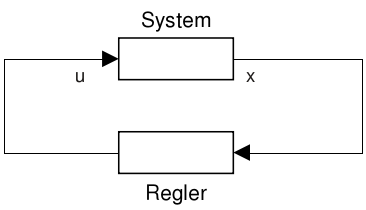
\includegraphics[scale=\modelscale]{rueckkopplung}
\end{center}

\pagebreak

\subsection{%
    Polvorgabe%
}

\textbf{Regelung durch lineare Zustandsrückführung}:
Bei einem System mit $x$-Dimension $n$ und $u$-Dimension $m$ ist
der \begriff{lineare Zustandsrückführungs-Regler (linear state-feedback controller)} definiert
durch $u = -Fx$ mit $F \in \real^{m \times n}$.

Für ein LTI-System $\dot{x} = Ax + Bu$ führt dies zu
$\dot{x} = Ax - BFx = (A - BF)x$
(\begriff{geschlossener Regelkreis (closed-loop system)} oder
\begriff{geregeltes System}).
Der Regler verändert daher die Dynamik des Systems vom ungeregelten System
$\dot{x} = Ax$ zum geregelten System $\dot{x} = (A - BF)x$.
Eine andere Interpretation ist, dass der Regler zur Zeit $t$ den Zustand $x(t)$ misst und
die Steuergröße $u(t) = -Fx(t)$ durch Bildung von Linearkombinationen der
Einträge von $x(t)$ berechnet.

\linie

Die Eigenwerte des Systems $\dot{x} = (A - BF)x$ bestimmen das
Verhalten des Systems.
Umso erstaunlicher ist es, dass bei regelbaren Systemen die Matrix $F$ stets so gewählt werden
kann, dass $A - BF$ beliebig vorgegebene Eigenwerte besitzt.
Weil diese eine Obermenge der Polstellen der Übertragungsmatrix darstellen, spricht man auch von
\begriff{Polvorgabe (pole placement)}.

\textbf{Satz (Polvorgabe)}:
Sei $(A, B)$ regelbar mit $A \in \real^{n \times n}$ und $B \in \real^{n \times m}$.\\
Wenn $\lambda_1, \dotsc, \lambda_n \in \complex$ (nicht notwendigerweise paarweise verschieden)
symmetrisch bzgl. der reellen Achse sind, dann gibt es eine Matrix $F \in \real^{m \times n}$
mit $\Eig(A - BF) = \{\lambda_1, \dotsc, \lambda_n\}$.

\linie

\textbf{Beweis für SI-Systeme}:
Ist $m = 1$, dann lässt sich $(A, B)$ in RKF bringen, d.\,h.\\
$\widetilde{A} = \smallpmatrix{-\alpha_1 & -\alpha_2 & \cdots & -\alpha_n \\
1 & 0 & & & \\ & \ddots & \ddots & & \\ 0 & & 1 & 0}$,
$\widetilde{B} = \smallpmatrix{1 \\ 0 \\ \vdots \\ 0}$ und
$\widetilde{A} - \widetilde{B} \widetilde{F} =
\smallpmatrix{-\alpha_1 - \widetilde{f}_1 & -\alpha_2 - \widetilde{f}_2 & \cdots &
-\alpha_n - \widetilde{f}_n \\
1 & 0 & & & \\ & \ddots & \ddots & & \\ 0 & & 1 & 0}$\\
mit $\widetilde{A} = TAT^{-1}$ und $\widetilde{B} = TB$ für $T \in \GL_n(\real)$ und
$\widetilde{F} = \smallpmatrix{\widetilde{f}_1 & \cdots & \widetilde{f}_n}
\in \real^{1 \times n}$.
Damit gilt\\
$\chi_{\widetilde{A} - \widetilde{B} \widetilde{F}}(s) =
s^n + (\alpha_1 + \widetilde{f}_1) s^{n-1} + \dotsb + (\alpha_n + \widetilde{f}_n)$.
Durch Wahl von $\widetilde{F}$ kann $\chi_{\widetilde{A} - \widetilde{B} \widetilde{F}}$
jedes beliebige reelle, normierte Polynom $n$-ten Grades sein,
also auch $(s - \lambda_1) \dotsm (s - \lambda_n)$.
Für $F := \widetilde{F} T$ gilt dann
$\widetilde{A} - \widetilde{B} \widetilde{F} = TAT^{-1} - TBFT^{-1} = T(A - BF)T^{-1}$,
somit $\chi_{A - BF} = \chi_{\widetilde{A} - \widetilde{B} \widetilde{F}}$.

Wenn man sich die Konstruktion von $S = T^{-1}$ im Beweis zur regelbar-kanonischen Form anschaut,
dann sieht man, dass $S = K T_\alpha$ mit
$K := \smallpmatrix{B & AB & \cdots & A^{n-1} B}$ der Kalman-Matrix und
$T_\alpha := \smallpmatrix{1 & \alpha_1 & \alpha_2 & \cdots & \alpha_{n-1} \\
& 1 & \alpha_1 & \cdots & \alpha_{n-2} \\
& & 1 & \cdots & \alpha_{n-3} \\
& & & \ddots & \vdots \\
0 & & & & 1}$.
Daher muss man $F = \smallpmatrix{\widetilde{f}_1 & \cdots & \widetilde{f}_n} [K T_\alpha]^{-1}$
wählen, wenn das charakteristische Polynom von $A - BF$ die Koef"|fizienten
$\alpha_1 + \widetilde{f}_1$, \dots, $\alpha_n + \widetilde{f}_n$ haben soll
(\begriff{\name{Bass}-\name{Gura}-Formel} oder \begriff{alternative \name{Ackermann}-Formel}).

\linie

\textbf{Beweis für MI-Systeme}:
Für den Beweis für $m > 1$ benötigt man zwei Lemmata.

\textbf{Lemma}:
Für $(A, B)$ regelbar
gibt es für alle $b \in R(B) \setminus \{0\}$ Vektoren $u_1, \dotsc, u_{n-1} \in \real^m$,
sodass $\{x_1, \dotsc, x_n\}$ linear unabhängig ist, wobei die $x_i$ definiert sind
durch $x_1 := b$ und die Rekursion $x_{i+1} := Ax_i + Bu_i$,
$i = 1, \dotsc, n - 1$.

Der Beweis erfolgt per Induktion:
Wegen $x_1 = b \not= 0$ ist $\{x_1\}$ l.u.
Seien $x_1, \dotsc, x_k$ l.u. mit $k < n$ und $V := [x_1, \dotsc, x_k]$.
Zeige $Ax_k + Bu_k \notin V$ für ein $u_k \in \real^m$ durch Widerspruch:
Angenommen, für alle $u \in \real^m$ gilt $Ax_k + Bu \in V$.
Dann gilt insbesondere $Ax_k \in V$ und somit $Bu \in V$ für alle $u \in \real^m$,
d.\,h. $R(B) \subset V$.
Damit gilt $Ax_i = x_{i+1} - Bu_i \in V$ für alle $i = 1, \dotsc, k - 1$,
zusätzlich gilt $Ax_k \in V$.
$V$ ist also $A$-invariant und enthält $R(B)$, d.\,h. $\real^n = R(K) \subset V$
aufgrund $(A, B)$ regelbar, ein Widerspruch zu $\dim V = k < n$.

\linie
\pagebreak

\textbf{\name{Heymann}-Lemma}:
Für $(A, B)$ regelbar
gibt es für alle $b \in R(B) \setminus \{0\}$ eine Matrix $F \in \real^{m \times n}$,
sodass $(A + BF, b)$ regelbar ist.

Seien $u_1, \dotsc, u_{n-1} \in \real^m$ so gewählt, dass die $x_1, \dotsc, x_n$
aus dem vorherigen Lemma linear unabhängig sind.
Für $u_n := 0$ sei $F := \smallpmatrix{u_1 & \cdots & u_n} \cdot
\smallpmatrix{x_1 & \cdots & x_n}^{-1}$.
Dann ist $Fx_i = u_i$ und somit $x_{i+1} = Ax_i + Bu_i = (A + BF)x_i$ für $i = 1, \dotsc, n - 1$.
Man erhält also $x_i = (A + BF)^{i-1} x_1 = (A + BF)^{i-1} b$ für $i = 1, \dotsc, n$.
Die Matrix $\smallpmatrix{x_1 & \cdots & x_n}$ ist daher die Kalman-Matrix von $(A + BF, b)$,
weil sie invertierbar ist (Spalten linear unabhängig), ist $(A + BF, b)$ regelbar.

\linie

\textbf{Beweis für MI-Systeme}:
Mit dem Heymann-Lemma folgt der Satz über die Polvorgabe:
Wähle $b \in R(B) \setminus \{0\}$
(wenn $B$ die Nullmatrix wäre, dann wäre $(A, B)$ nicht regelbar).
Sei $\widetilde{F} \in \real^{m \times n}$ nach dem Heymann-Lemma, sodass
$(A + B\widetilde{F}, b)$ regelbar ist.
Wähle $\widehat{F} \in \real^{1 \times n}$, sodass
$\Eig((A + B\widetilde{F}) - b\widehat{F}) = \{\lambda_1, \dotsc, \lambda_n\}$
(geht nach dem schon bewiesenen Fall $m = 1$).
Wegen $b \in R(B)$ gibt es $u_0 \in \real^m$ mit $Bu_0 = b$.
Definiere $F := u_0 \widehat{F} - \widetilde{F}$.
Damit gilt $A - BF = A + B\widetilde{F} - Bu_0\widehat{F}
= A + B\widetilde{F} - b\widehat{F}$,
d.\,h. $A - BF$ besitzt die gewünschten Eigenwerte.

\linie

\textbf{unregelbare Systeme}:
Jedes System $(A, B)$ kann in Regelbarkeits-Normalform
$(\widetilde{A}, \widetilde{B})$ gebracht werden.
Wenn $\widetilde{F}$ eine Rückführungsverstärkung für das transformierte System ist,
dann können die Spalten von $\widetilde{F} = \smallpmatrix{\widetilde{F}_1 & \widetilde{F}_2}$
wie die von $\widetilde{A}$ eingeteilt werden.
Mit $u = -\widetilde{F}z$ erhält man das System
$\smallpmatrix{\dot{z}_1 \\ \dot{z}_2} = \smallpmatrix{A_{11} - B_1\widetilde{F}_1 &
A_{12} - B_1 \widetilde{F}_2 \\ 0 & A_{22}} \smallpmatrix{z_1 \\ z_2}$.
Weil $(A_{11}, B_1)$ regelbar ist, können die Eigenwerte von $A_{11} - B_1\widetilde{F}_1$
durch geeignete Wahl von $\widetilde{F}_1$ beliebig gewählt werden.
Daher wählt man $\widetilde{F}_1$ immer so, dass sie alle negativen Realteil haben.
Die Eigenwerte von $A_{22}$ kann man durch die lineare Zustandsregelung nicht beeinflussen,
was die Bezeichnung "`unregelbare Eigenwerte"' noch einmal rechtfertigt.
Für $(A, B)$ unregelbar gibt es also immer Eigenwerte von $A - BF$, die fest sind
und nicht durch $F$ verschoben werden können.

\linie

\textbf{Satz (Stabilisierung durch lineare Zustandsrückführung)}:
Das System $\dot{x} = Ax + Bu$ ist stabilisierbar genau dann, wenn
es eine Matrix $F \in \real^{m \times n}$ gibt, sodass $\dot{x} = (A - BF)x$
asymptotisch stabil ist (d.\,h. $A - BF$ ist eine Hurwitz-Matrix).

\subsection{%
    \emph{Zusatz}: Kanonische \name{Brunovsky}-Form%
}

\textbf{äquivalent}:
Die Paare $(A, B)$ und $(\widetilde{A}, \widetilde{B})$
(mit $A, \widetilde{A} \in \real^{n \times n}$ und
$B, \widetilde{B} \in \real^{n \times m}$) heißen \begriff{äquivalent},
falls es Matrizen $S \in \real^{n \times n}$ invertierbar, $U \in \real^{m \times m}$
invertierbar und $F \in \real^{m \times n}$ gibt, sodass
$S^{-1} \smallpmatrix{A & B} \smallpmatrix{S & 0 \\ -F & U} =
\smallpmatrix{\widetilde{A} & \widetilde{B}}$.

Man kann das auch schreiben als
$\widetilde{A} = S^{-1} AS - S^{-1} BF$ und $\widetilde{B} = S^{-1} BU$.
Äquivalent dazu kann man auch $-F$ durch $-FS$ ersetzen.
Äquivalenz von Paaren $(A, B)$ ist eine Äquivalenzrelation
auf der Menge $\real^{n \times n} \times \real^{n \times m}$ der Paare $(A, B)$.
$(\widetilde{A}, \widetilde{B})$ ist regelbar genau dann, wenn $(A, B)$ regelbar ist.

\textbf{Spezialfälle}:
\begin{enumerate}
    \item
    \emph{Zustandskoordinaten-Transformation} ($F = 0$, $U = I$):
    $\widetilde{A} = S^{-1} AS$ und $\widetilde{B} = S^{-1} B$\\
    (zugehöriges System $\dot{z} = S^{-1} ASz + S^{-1} Bu$)
    
    \item
    \emph{Eingangskoordinaten-Transformation} ($S = I$, $F = 0$):
    $\widetilde{A} = A$ und $\widetilde{B} = BU$\\
    (zugehöriges System $\dot{x} = Ax + BUv$ mit $u = Uv$)
    
    \item
    \emph{lineare Zustandsrückführung, neuer Eingang} ($S = I$, $U = I$):
    $\widetilde{A} = A - BF$ und $\widetilde{B} = B$\\
    (zugehöriges System $\dot{x} = (A - BF)x + Bv$ mit $u = -Fx + v$)
\end{enumerate}

\linie
\pagebreak

\textbf{Äquivalenz als Gruppenoperation}:
Wegen $\smallpmatrix{S_1 & 0 \\ -F_1 & U_1} \cdot \smallpmatrix{S_2 & 0 \\ -F_2 & U_2}
= \smallpmatrix{S_3 & 0 \\ -F_3 & U_3}$
mit $S_3 := S_1 S_2$ invertierbar, $U_3 = U_1 U_2$ invertierbar und
$F_3 := F_1 S_2 + U_1 F_2$ ist die Menge $G$ der
Blockmatrizen $\smallpmatrix{S & 0 \\ -F & U}$
mit $S$ und $U$ invertierbar eine Gruppe bzgl. der Multiplikation
(man braucht zusätzlich noch $\smallpmatrix{I & 0 \\ 0 & I} \in G$ und
$\smallpmatrix{S & 0 \\ -F & U}^{-1} = \smallpmatrix{S^{-1} & 0 \\ U^{-1}FS^{-1} & U^{-1}} \in G$).
Diese Gruppe definiert eine Gruppenoperation auf der Menge
$\real^{n \times n} \times \real^{n \times m}$ der Paare von Matrizen $(A, B)$:\\
$\smallpmatrix{S & 0 \\ -F & U} \cdot (A, B) := (\widetilde{A}, \widetilde{B})
= (S^{-1} AS - S^{-1} BF, S^{-1} BU)$.
Die Bahnen unter dieser Operation sind genau die Äquivalenzklassen der obigen Äquivalenz.

\linie

\textbf{Satz (kanonische \name{Brunovsky}-Form)}:
Sei $(A, B)$ regelbar, wobei $B \in \real^{n \times m}$ vollen Spaltenrang hat.
Dann gibt es $\kappa_1, \dotsc, \kappa_m \in \natural$ mit
$\kappa_1 \ge \dotsb \ge \kappa_m$
(\begriff{Regelbarkeits-Indizes (controllability indices)}),
sodass $(A, B)$ zu $(\widetilde{A}, \widetilde{B})$
äquivalent ist mit
\begin{align*}
    \widetilde{A} =
    \smallpmatrix{
        0 & 0 & \dotsb & 0 & & & & & 0 \\
        1 & 0 & & 0 & & & & & \\
        & \ddots & \ddots & \vdots & & & & & \\
        0 & & 1 & 0 & & & & & \\
        & & & & \ddots & & & & \\
        & & & & & 0 & 0 & \dotsb & 0 \\
        & & & & & 1 & 0 & & 0 \\
        & & & & & & \ddots & \ddots & \vdots \\
        0 & & & & & 0 & & 1 & 0
    },\quad
    \widetilde{B} =
    \smallpmatrix{
        1 & & 0 \\
        0 & & \\
        \vdots & & \\
        0 & & \\
        & \ddots & \\
        & & 1 \\
        & & 0 \\
        & & \vdots \\
        0 & & 0
    },
\end{align*}
wobei die Dimensionen der Kästchen $\kappa_i \times \kappa_i$ bzw. $\kappa_i \times 1$ sind
($i = 1, \dotsc, m$).\\
Diese Form heißt \begriff{kanonische \name{Brunovsky}-Form (\name{Brunovsky} canonical form)}.

Falls $B$ nicht vollen Spaltenrang hat, dann gibt es eine Eingangskoordinaten-Transformation
$Uv = u$ mit $U$ invertierbar, sodass $BU = \smallpmatrix{\widetilde{B}_1 & 0}$ gilt und
$\widetilde{B}_1$ vollen Spaltenrang hat.
In diesem Fall ist $Bu = BUv = \smallpmatrix{\widetilde{B}_1 & 0} \smallpmatrix{v_1 \\ v_2}
= \widetilde{B}_1 v_1$, d.\,h. der Teil $v_2$ des neuen Eingangs ist nicht relevant.
Daher nimmt man in der Literatur oft oBdA an, dass $B$ vollen Spaltenrang hat.

\textbf{\name{Brunovsky}-Form ohne lineare Zustandsregelung}:\\
Man kann obigen Satz auch ohne lineare Zustandsregelung formulieren (d.\,h. $F = 0$).\\
Es gibt eine Zustands- und Eingangskoordinaten-Transformation von $(A, B)$ in
$(\widetilde{A}, \widetilde{B})$ mit
\begin{align*}
    \widetilde{A} =
    \smallpmatrix{
        \ast & \ast & \cdots & \ast & \cdots & \cdots & \cdots & \cdots & \ast \\
        1 & 0 & & 0 & & & & & \\
        & \ddots & \ddots & \vdots & & & & & \\
        0 & & 1 & 0 & & & & & \\
        & & & & \ddots & & & & \\
        \ast & \cdots & \cdots & \cdots & \cdots & \ast & \ast & \cdots & \ast \\
        & & & & & 1 & 0 & & 0 \\
        & & & & & & \ddots & \ddots & \vdots \\
        0 & & & & & 0 & & 1 & 0
    },\quad
    \widetilde{B} =
    \smallpmatrix{
        1 & & 0 \\
        0 & & \\
        \vdots & & \\
        0 & & \\
        & \ddots & \\
        & & 1 \\
        & & 0 \\
        & & \vdots \\
        0 & & 0
    }.
\end{align*}

\linie

\textbf{Polvorgabe mit kanonischer \name{Brunovsky}-Form}:
Mit der kanonischen Brunovsky-Form ist der Satz über die Polvorgabe einfach zu zeigen
(allerdings ist der Satz über die kanonische Brunovsky-Form relativ aufwendig zu beweisen):
Für $\widetilde{F} \in \real^{m \times n}$ beliebig ist $\widetilde{B}\widetilde{F}$
eine $(n \times n)$-Matrix, die nur Nullen enthält, außer in den $\ast$-Zeilen von $\widetilde{A}$
(dort stehen die Zeilen von $\widetilde{F}$).
Somit kann man die Elemente von $\widetilde{F}$, die zu Einträgen von $\widetilde{A}$ außerhalb von
Blöcken gehören, so wählen, dass die $\ast$-Zeilen außerhalb der Blöcke $\widetilde{A}_i$
verschwinden.
Die übrigen Einträge von $\widetilde{F}$ (in den Blöcken $\widetilde{F}_i$) wählt man so, dass
$\widetilde{A}_i - \widetilde{B}_i \widetilde{F}_i$
die gewünschten Eigenwerte besitzt, was aufgrund der Polvorgabe für SI-Systeme möglich ist.
Damit besitzt auch $\widetilde{A} - \widetilde{B} \widetilde{F}$ die gewünschten Eigenwerte.
Wegen\\
$\widetilde{A} - \widetilde{B} \widetilde{F}
= S^{-1}AS - S^{-1}BF - S^{-1}BU \widetilde{F}
= S^{-1}AS - S^{-1}B(F + U\widetilde{F})
= S^{-1} (A - B\widehat{F}) S$
mit $\widehat{F} := (F + U\widetilde{F}) S^{-1}$
besitzt auch $A - B\widehat{F}$ die geforderten Eigenwerte.

\pagebreak

\subsection{%
    Dominante Eigenwerte%
}

\textbf{Dämpfungsverhältnis}:
Das \begriff{Dämpfungsverhältnis (damping ratio)} des nicht-reellen Eigenwerts
$\lambda \in \Eig(A) \setminus \real$ von $A$ ist definiert als
$\zeta := -\frac{\Re(\lambda)}{|\lambda|}$.

\textbf{dominanter Eigenwert}:
Ein Paar von nicht-reellen Eigenwerten $\lambda, \overline{\lambda} \in \Eig(A) \setminus \real$
von $A$ heißt \begriff{dominant}, falls ihr Dämpfungsverhältnis das kleinste aller
Dämpfungsverhältnisse von nicht-reellen Eigenwerten von $A$ ist.

Für Hurwitz-Matrizen $A$ ist das Verhalten von $t \mapsto e^{At}$ häufig (aber nicht immer)
hauptsächlich bestimmt durch den dominanten Eigenwert von $A$.
Wegen der reellen Jordan-Normalform von $A$ ist $e^{At}$ eine Überlagerung von $e$-Funktionen
mit reellen Exponenten oder von $e^{Jt}$ mit $(2 \times 2)$-Blöcken $J$ mit
nicht-reellen Eigenwerten.
Ist ein solcher Block $J$ eine Hurwitz-Matrix, dann bestimmt das Dämpfungsverhältnis die
Dominanz der Antwort.

\linie

\textbf{Platzierung der Eigenwerte}:
Diese Frage ist nicht leicht zu beantworten.
\begin{itemize}
    \item
    Die Bass-Gura-Formel
    $F = \smallpmatrix{\widetilde{f}_1 & \cdots & \widetilde{f}_n} [K T_\alpha]^{-1}$
    zeigt:
    Je kleiner die Verschiebung der Koef"|fizienten des charakteristischen Polynoms
    (und der Eigenwerte) ist, desto kleiner sind die Koef"|fizienten von $F$ --
    was wünschenswert ist, denn große Koef"|fizienten bedeuten einen großen Regelaufwand.
    
    \item
    Die Rolle von dominanten Eigenwerten führt zum folgenden Design-Rezept:
    \begin{itemize}
        \item
        Wähle ein System zweiter Ordnung mit der gewünschten Dynamik.
        
        \item
        Platziere zwei Eigenwerte an den zwei Polstellen des Systems.
        
        \item
        Wähle alle anderen Eigenwerte schneller (damit sie weniger dominant sind),
        aber nicht zu schnell (um zu starken Regelaufwand zu vermeiden).
        
        \item
        Platziere die Eigenwerte und überprüfe mittels dynamischer Simulation.
    \end{itemize}
    Üblicherweise muss man diesen Vorgang mehrmals wiederholen,
    um gute Ergebnisse zu erzielen.
\end{itemize}

\pagebreak

\chapter{%
    Beobachtbarkeit und das Separationsprinzip%
}

\section{%
    Beobachtbarkeit und Dualität%
}

\textbf{Rekonstruktion des Zustands}:
Bei linearen System $\dot{x} = Ax + Bu$ kann in der Praxis eigentlich nie davon ausgegangen werden,
dass alle Komponenten des Zustands messbar sind und zur Verfügung stehen.
Daher kennt man normalerweise nur den Ausgang $y = Cx + Du$
als dem Regler verfügbare Information.
Ist es möglich, nur aus dem Wissen von $u$ und $y$ den Zustand $x$ zu rekonstruieren?
Kann mit dem rekonstruierten Zustand ein Regler implementiert werden?

\textbf{beobachtbar}:
Das lineare System $\dot{x} = Ax + Bu$, $y = Cx + Du$ heißt \begriff{beobachtbar (observable)},
falls es für jedes $T > 0$ möglich ist, $x(t)$ für $t \in [0, T]$ aus
$u(t)$ und $y(t)$ für $t \in [0, T]$ zu rekonstruieren.

\linie

$y$ hat normalerweise viel weniger Komponenten als $x$.
Daher ist die Rekonstruktion direkt aus $y$ unmöglich.
Allerdings kann man $y$ ableiten, um $y(t), \dot{y}(t), \dotsc, y^{(n-1)}(t)$ zu erhalten
(zumindest in der Theorie, in der Praxis ist das kaum möglich).
Es gilt $Y(t) = W x(t) + \D U(t)$ mit\\
$Y(t) := \smallpmatrix{y(t) \\ \dot{y}(t) \\ \vdots \\ y^{(n-1)}(t)}$,
$W := \smallpmatrix{C \\ CA \\ \vdots \\ CA^{n-1}}$,
$\D := \smallpmatrix{D & & & 0 \\ CB & D & & \\ \vdots & \ddots & \ddots & \\
C A^{n-2} B & \cdots & CB & D}$ und
$U(t) := \smallpmatrix{u(t) \\ \dot{u}(t) \\ \vdots \\ u^{(n-1)}(t)}$.

\textbf{Beobachtbarkeitsmatrix}:
$W$ heißt \begriff{Beobachtbarkeitsmatrix (observability matrix)} des Systems
$\dot{x} = Ax + Bu$, $y = Cx + Du$
oder des Paars $(A, C)$.

\linie

Wenn $W$ vollen Spaltenrang hat, dann gibt es eine Matrix $W^+$ mit $W^+ W = I$,
d.\,h.\\
$W^+ Y(t) = x(t) + W^+ \D U(t) \iff x(t) = W^+ Y(t) - W^+ \D U(t)$,
also kann man $x(t)$ aus $Y(t)$ und $U(t)$ rekonstruieren.
Es gilt aber auch die Umkehrung.

\textbf{Satz (\name{Kalman}-Test zur Beobachtbarkeit)}:
Das lineare System $\dot{x} = Ax + Bu$, $y = Cx + Du$ ist beobachtbar genau dann,
wenn die Beobachtbarkeitsmatrix $W$ vollen Spaltenrang hat.

$W^T = \smallpmatrix{C^T & A^T C^T & \cdots & (A^T)^{n-1} C^T}$ ist die Kalman-Matrix
von $(A^T, C^T)$.
Daher gilt $(A, C)$ beobachtbar $\iff$ $W$ hat vollen Spaltenrang $\iff$ $W^T$ hat vollen
Zeilenrang $\iff$ $(A^T, C^T)$ ist regelbar.
Man kann also alle Sätze und Eigenschaften über die Regelbarkeit von $(A^T, C^T)$ auf
die Beobachtbarkeit von $(A, C)$ übertragen.

\textbf{Dualitätsprinzip}:
Das \begriff{Dualitätsprinzip (duality principle)}
der linearen Kontrolltheorie ist die Übersetzung von Fragen
der Beobachtbarkeit von $(A, B, C, D)$ in Fragen der Regelbarkeit von $(A^T, C^T, B^T, D^T)$
(oder umgekehrt).

\textbf{Satz (\name{Hautus}-Test zur Beobachtbarkeit)}:
$(A, C)$ ist beobachtbar genau dann, wenn für jeden Eigenvektor $e$ von $A$ gilt,
dass $Ce \not= 0$.
Äquivalent dazu ist, dass die Matrix $\smallpmatrix{A - \lambda I \\ C}$
vollen Spaltenrang für alle $\lambda \in \complex$ besitzt.

\pagebreak

\section{%
    Unbeobachtbarer Unterraum und Eigenwert%
}

Wenn $W$ nicht vollen Spaltenrang hat, dann ist $N(W) \not= \{0\}$.
Nicht-verschwindende Trajektorien in diesem Raum werden von $W$ "`verschluckt"'
und können daher im Ausgang nicht beobachtet werden.

\textbf{unbeobachtbarer Unterraum}:\\
$N(W)$ heißt \begriff{unbeobachtbarer Unterraum (unobservable subspace)} von $(A, C)$.

\textbf{unbeobachtbarer Eigenwert}:
Ein \begriff{unbeobachtbarer Eigenwert (unobservable mode)} von $(A, C)$ ist
$\lambda \in \complex$, sodass $\smallpmatrix{A - \lambda I \\ C}$ nicht vollen Spaltenrang hat.

\linie

\textbf{Satz (geometrische Charakterisierung von $N(W)$)}:
Der unbeobachtbare Unterraum von $(A, C)$ ist der größte $A$-invariante Unterraum,
der in $N(C)$ enthalten ist.

\textbf{Satz (Beobachtbarkeits-Normalform)}:
Es gibt eine Zustandskoordinaten-Transformation $z = Tx$ mit $T$ invertierbar,
die $\dot{x} = Ax + Bu$, $y = Cx + Du$ in
$\smallpmatrix{\dot{z}_1 \\ \dot{z}_2} = \smallpmatrix{A_{11} & 0 \\ A_{21} & A_{22}}
\smallpmatrix{z_1 \\ z_2} + \smallpmatrix{B_1 \\ B_2} u =: \widetilde{A}z + \widetilde{B}u$,
$y = \smallpmatrix{C_1 & 0} \smallpmatrix{z_1 \\ z_2} + Du =: \widetilde{C} z + Du$ transformiert,
wobei $(A_{11}, C_1)$ beobachtbar ist.
Diese Form heißt \begriff{Beobachtbarkeits-Normalform (observability normal form)}
oder \begriff{BNF}.

Ausgeschrieben bedeutet das $\dot{z}_1 = A_{11} z_1 + B_1 u$,
$\dot{z}_2 = A_{21} z_1 + A_{22} z_2 + B_2 u$, $y = C_1 z_1 + Du$,
d.\,h. $z_1$ und daher auch $y$ werden von $z_2$ nicht beeinflusst.
Beispielsweise lässt sich eine Veränderung der Anfangsbedingung $z_2(0)$ nicht in $y$ beobachten.

\textbf{Folgerung}:
Der unbeobachtbare Unterraum von $(\widetilde{A}, \widetilde{C})$ ist
$\{(0, z_2) \;|\; z_2 \in \real^{\dim(z_2)}\}$ und die unbeobachtbaren Eigenwerte sind
die Eigenwerte von $A_{22}$.

Es gibt viele Gründe für Unbeobachtbarkeit.
Wenn man z.\,B. zwei identische, beobachtbare Systeme $(A_S, B_S, C_S, D_S)$ durch
Parallelschaltung (mit unterschiedlichen Eingängen) verknüpft,
erhält man $\dot{x} = Ax + Bu$, $y = Cx + Du$ mit
$A := \smallpmatrix{A_S & 0 \\ 0 & A_S}$,
$B := \smallpmatrix{B_S & 0 \\ 0 & B_S}$,
$C := \smallpmatrix{C_S & C_S}$ und
$D := \smallpmatrix{D_S & D_S}$.
Die Beobachtbarkeitsmatrix von $(A, C)$ hat
zwei identische Blockspalten und kann daher keinen vollen Spaltenrang haben.
Wenn $A_S$ die Dimension $n$ hat, dann ist der unbeobachtbare Unterraum von $(A, C)$ gleich
$\left\{\left.\smallpmatrix{x \\ -x} \;\right| x \in \real^n\right\}$.

\linie

\textbf{Satz (beobachtbar-kanonische Form)}:
Wenn $\dot{x} = Ax + Bu$, $y = Cx + Du$ nur einen Ausgang hat (d.\,h. $y$ ist skalar)
und beobachtbar ist, dann gibt es einen Koordinatenwechsel $z = Tx$ mit $T$ invertierbar,
der das System in
$\dot{z} = \smallpmatrix{-\alpha_1 & 1 & & & 0 \\ -\alpha_2 & 0 & 1 & & \\
\vdots & & \ddots & \ddots & \\ -\alpha_{n-1} & & & 0 & 1 \\ -\alpha_n & & & & 0} z
+ \widetilde{B} u := \widetilde{A} z + \widetilde{B} u$,
%+ \smallpmatrix{b_1 \\ b_2 \\ \vdots \\ b_{n-1} \\ b_n} u := \widetilde{A} z + \widetilde{B} u$,
$y = \smallpmatrix{1 & 0 & 0 & \cdots & 0} z + Du = \widetilde{C} z + Du$ transformiert.\\
Diese Form heißt \begriff{beobachtbar-kanonische Form (observability canonical form)}
oder \begriff{BKF}.

\pagebreak

\section{%
    Beobachter und Entdeckbarkeit%
}

Die sofortige Rekonstruktion des Zustands ist praktisch nicht möglich, da Rauschen durch die
Dif"|ferentiation verstärkt wird.
Außerdem kann die Beobachtbarkeitsmatrix schlecht konditioniert sein.
Daher versucht man, den Zustand asymptotisch zu rekonstruieren.

\textbf{Beobachter}:
Ein \begriff{Beobachter (observer)} für das lineare System $\dot{x} = Ax + Bu$, $y = Cx + Du$
ist das dynamische System
$\dotwidehat{x} = A\widehat{x} + Bu + L(y - \widehat{y})$, $\widehat{y} = C\widehat{x} + Du$.

Ein Beobachter ist eine Kopie des Originalsystems mit einem Korrekturterm $L(y - \widehat{y})$,
der dazu dient, dass der geschätzte Zustand $\widehat{x}$ in Richtung $x$ geregelt wird
(für den Fall, dass sich der gemessene Ausgang $y$ vom geschätzten Ausgang $\widehat{y}$
unterscheidet).

\textbf{Bestimmung von $L$}:
Natürlich sollte der \begriff{Schätzfehler} $\widetilde{x} := x - \widehat{x}$ schnell gegen
Null konvergieren.
Für seine Dynamik gilt
$\dotwidetilde{x} = \dot{x} - \dotwidehat{x} =
Ax + Bu - A\widehat{x} - Bu - L(y - \widehat{y})$\\
$= A\widetilde{x} - L(Cx + Du - C\widehat{x} - Du)
= (A - LC) \widetilde{x}$ (\begriff{Fehlerdynamik}).
Daher sollte $L$ so gewählt werden, dass $A - LC$ eine Hurwitz-Matrix ist, damit
$\lim_{t \to \infty} \widetilde{x}(t) = 0$.
Die Konvergenzgeschwindigkeit und die Art der Antwort (z.\,B. das Überschwingen)
hängt von den Eigenwerten von $A - LC$ ab und von $e^{(A - LC)t}$.

\textbf{Satz (Polvorgabe für Beobachter)}:\\
Seien $(A, C)$ beobachtbar und $\alpha$ ein reelles, normiertes
Polynom vom Grad $n$.\\
Dann gibt es eine reelle Matrix $L$ mit $\chi_{A - LC} = \alpha$.

\linie

\textbf{entdeckbar}:
Das System $\dot{x} = Ax + Bu$, $y = Cx + Du$ (oder das Paar $(A, C$) heißt
\begriff{entdeckbar (detectable)},
falls es eine Matrix $L$ gibt, sodass $A - LC$ eine Hurwitz-Matrix ist.

\textbf{Satz (\name{Hautus}-Test zur Entdeckbarkeit)}:
$(A, C)$ ist entdeckbar genau dann, wenn
die unbeobachtbaren Eigenwerte alle negative Realteile besitzen.
Äquivalent dazu ist, dass $\smallpmatrix{A - \lambda I \\ C}$ vollen Spaltenrang für alle
$\lambda \in \complex$ mit $\Re(\lambda) \ge 0$ besitzt.

\textbf{Satz (Trajektorien-basierte Charakterisierung)}:
Das System $\dot{x} = Ax + Bu$, $y = Cx + Du$ ist entdeckbar genau dann, wenn
$u(t) \equiv 0$ und $y(t) \equiv 0$ für $t \ge 0$ implizieren, dass\\
$\lim_{t \to \infty} x(t) = 0$.

\begin{landscape}
\section{%
    \emph{Zusatz}: Zusammenfassung der Dualität%
}

\newcommand*{\tablelinespace}{2mm}
\small
\begin{tabular}{p{35mm}p{105mm}p{105mm}}
    \toprule
    &
    \textbf{Regelbarkeit} &
    \textbf{Beobachtbarkeit}\\

    \midrule
    \emph{Traj.-Definition} &
    für jedes $x_f \in \real^n$ existiert $u$ stetig, sodass $x(T) = x_f$\newline
    für $x(0) = 0$ und $T > 0$ fest &
    %von jedem $\xi \in \real^n$ für $t = 0$ kann in jedes $x_f \in \real^n$ für $t = T > 0$\newline
    %gesteuert werden &
    für jedes $T > 0$ ist die Rekonstruktion von $x(t)$ für $t \in [0, T]$\newline
    aus $u(t)$ und $y(t)$ für $t \in [0, T]$ möglich\\

    \addlinespace[\tablelinespace]
    \emph{Dualität} &
    \multicolumn{2}{c}{$(A^T, C^T)$ regelbar $\iff$ $(A, C)$ beobachtbar}\\

    \addlinespace[\tablelinespace]
    \emph{\name{Kalman}-Test} &
    $K = \smallpmatrix{B & AB & \cdots & A^{n-1}B}$ hat vollen Zeilenrang &
    $W = \smallpmatrix{C \\ CA \\ \vdots \\ CA^{n-1}}$ hat vollen Spaltenrang\\

    \addlinespace[\tablelinespace]
    \emph{Unterraum} &
    $R(K)$ regelbarer Unterraum &
    $N(W)$ unbeobachtbarer Unterraum\\

    \addlinespace[\tablelinespace]
    \emph{geom. Charakter.} &
    kleinster $A$-invarianter Unterraum, der $R(B)$ enthält &
    größter $A$-invarianter Unterraum, der in $N(C)$ enthalten ist\\

    \addlinespace[\tablelinespace]
    \emph{\name{Hautus}-Test} &
    $\smallpmatrix{A - \lambda I & B}$ hat vollen Zeilenrang für alle $\lambda \in \complex$ &
    $\smallpmatrix{A - \lambda I \\ C}$ hat vollen Spaltenrang für alle $\lambda \in \complex$\\

    \addlinespace[\tablelinespace]
    \emph{Eigenwerte} &
    $\lambda \in \complex$ mit Rangverlust unregelbare Eigenwerte &
    $\lambda \in \complex$ mit Rangverlust unbeobachtbare Eigenwerte\\

    \addlinespace[\tablelinespace]
    \emph{Polvorgabe} &
    für regelbare Systeme für $A - BF$ möglich &
    für beobachtbare Systeme für $A - LC$ möglich\\

    \addlinespace[\tablelinespace]
    \emph{kanonische Form\newline($m = 1$ bzw. $k = 1$)} &
    $\dot{z} = \smallpmatrix{-\alpha_1 & -\alpha_2 & \cdots & -\alpha_n \\
    1 & 0 & & & \\ & \ddots & \ddots & & \\ 0 & & 1 & 0} z +
    \smallpmatrix{1 \\ 0 \\ \vdots \\ 0} u$
    &
    $\dot{z} = \smallpmatrix{-\alpha_1 & 1 & & & 0 \\ -\alpha_2 & 0 & 1 & & \\
    \vdots & & \ddots & \ddots & \\ -\alpha_{n-1} & & & 0 & 1 \\ -\alpha_n & & & & 0} z
    + \widetilde{B} u$,
    $y = \smallpmatrix{1 & 0 & 0 & \cdots & 0} z + Du$\\

    \addlinespace[\tablelinespace]
    \emph{Normalform} &
    $\smallpmatrix{\widetilde{A} & \widetilde{B} \\ \widetilde{C} & \widetilde{D}}
    = \smallpmatrix{A_{11} & A_{12} & B_1 \\ 0 & A_{22} & 0 \\ C_1 & C_2 & D}$,
    $(A_{11}, B_1)$ regelbar &
    $\smallpmatrix{\widetilde{A} & \widetilde{B} \\ \widetilde{C} & \widetilde{D}}
    = \smallpmatrix{A_{11} & 0 & B_1 \\ A_{21} & A_{22} & B_2 \\ C_1 & 0 & D}$,
    $(A_{11}, C_1)$ beobachtbar\\

    \addlinespace[\tablelinespace]
    \midrule
    &
    \textbf{Stabilisierbarkeit} &
    \textbf{Entdeckbarkeit}\\

    \midrule
    \emph{Traj.-Definition} &
    für jedes $\xi \in \real^n$ existiert $u$ stückweise stetig, sodass\newline
    $\lim_{t \to \infty} x(t) = 0$ für $x(0) = \xi$ &
    aus $u(t) \equiv 0$ und $y(t) \equiv 0$ für $t \ge 0$ folgt $\lim_{t \to \infty} x(t) = 0$\\

    \addlinespace[\tablelinespace]
    \emph{Dualität} &
    \multicolumn{2}{c}{$(A^T, C^T)$ stabilisierbar $\iff$ $(A, C)$ entdeckbar}\\

    \addlinespace[\tablelinespace]
    \emph{Verallgemeinerung} &
    regelbar impliziert stabilisierbar &
    beobachtbar impliziert entdeckbar\\

    \addlinespace[\tablelinespace]
    \emph{\name{Hautus}-Test} &
    $\smallpmatrix{A - \lambda I & B}$ hat vollen Zeilenrang für alle
    $\lambda \in \complex$ mit $\Re(\lambda) \ge 0$ &
    $\smallpmatrix{A - \lambda I \\ C}$ hat vollen Spaltenrang für alle $\lambda \in \complex$
    mit $\Re(\lambda) \ge 0$\\

    \addlinespace[\tablelinespace]
    \emph{alg. Charakter.} &
    es gibt eine Matrix $F$ mit $A - BF$ Hurwitz-Matrix &
    es gibt eine Matrix $L$ mit $A - LC$ Hurwitz-Matrix\\

    \addlinespace[\tablelinespace]
    \bottomrule
\end{tabular}
\end{landscape}

\section{%
    Das Separationsprinzip%
}

Es wurde schon gezeigt, wie man ein System durch lineare Zustandsrückführung stabilisieren kann.
Allerdings benötigt diese Regelung den kompletten Zustand zu jeder Zeit.
Es wurde ebenfalls schon gezeigt, wie man den Zustand durch den gemessenen Ausgang
asymptotisch rekonstruieren kann.
Diese Techniken lassen sich enorm ef"|fizient miteinander verbinden:

Für ein stabilisierbares und entdeckbares LTI-System $\dot{x} = Ax + Bu$, $y = Cx + Du$
seien $F$ und $L$, sodass $A - BF$ und $A - LC$ Hurwitz-Matrizen sind.
Dann stabilisiert $u = -Fx$ das System und der Beobachter mit Verstärkung $L$ erzeugt eine
Zustandsschätzung $\widehat{x}$, die $x$ asymptotisch rekonstruiert.
Die Schlüsselidee ist es nun, das nicht verfügbare $x$ durch die verfügbare Schätzung
$\widehat{x}$ zu ersetzen, d.\,h. $u = -F\widehat{x}$.

\linie

\textbf{beobachterbasierter Ausgangsrückführungs-Regler}:
Für die Design-Parameter $F$ und $L$ ist das lineare System
$\dotwidehat{x} = A\widehat{x} + Bu + L(y - \widehat{y})$,
$\widehat{y} = C\widehat{x} + Du$, $u = -F\widehat{x}$
ein\\
\begriff{beobachterbasierter Ausgangsrückführungs-Regler
(observer-based output-feedback controller)}.

Äquivalente Implementierungen sind
$\dotwidehat{x} = (A - LC) \widehat{x} + (B - LD)u + Ly$, $u = -F\widehat{x}$ und
$\dotwidehat{x} = (A - LC - BF + LDF) \widehat{x} + Ly$, $u = -F\widehat{x}$.

\textbf{Satz (geschlossener Regelkreis)}:
Die Verbindung des beobachterbasierten Ausgangsrück"-führungs-Regler mit dem ursprünglichen
System führt zum geschlossenen Regelkreis\\
$\dot{x}  = Ax - BF\widehat{x}$,
$\dotwidehat{x} = (A - LC - BF) \widehat{x} + LCx$.
Dieses System ist asymptotisch stabil genau dann, wenn $A - BF$ und $A - LC$ Hurwitz-Matrizen sind.

Den Satz sieht man sehr schnell durch die Transformation
$\smallpmatrix{x \\ \widetilde{x}} = T \smallpmatrix{x \\ \widehat{x}}$ mit
$T := \smallpmatrix{I & 0 \\ I & -I} = T^{-1}$.
Damit ergibt sich $T \smallpmatrix{A & -BF \\ LC & A - LC - BF} T^{-1} = \A
:= \smallpmatrix{A - BF & BF \\ 0 & A - LC}$, d.\,h. die Eigenwerte des Systems
$\smallpmatrix{\dot{x} \\ \dotwidetilde{x}} = \A \smallpmatrix{x \\ \widetilde{x}}$
sind gleich denen von $A - BF$ vereinigt mit denen von $A - LC$.

\linie

\textbf{statische Ausgangsrückführung}:\\
Bei der \begriff{statischen Ausgangsrückführung (static output-feedback)} des Systems
$\dot{x} = Ax + Bu$, $y = Cx$ setzt man $u = -Ky$.
Man erhält also $\dot{x} = (A - BKC)x$ als geschlossenen Regelkreis.
Bis heute existiert kein einfacher Test,
unter welchen Bedingungen $A - BKC$ Hurwitz ist.

\linie

\textbf{Zusammenfassung}:
\begin{itemize}
    \item
    Überprüfe, ob $(A, B)$ stabilisierbar und $(A, C)$ entdeckbar ist.
    Falls nicht, so kann man zeigen, dass kein linearer, stabilisierender Regler existiert.

    \item
    Falls ja, bestimme $F$ und $L$, sodass $A - BF$ und $A - LC$ Hurwitz-Matrizen sind.

    \item
    Der beobachterbasierte Regler führt zu einem System mit Eigenwerten\\
    $\Eig(A - BF) \cup \Eig(A - LC)$.

    \item
    Wenn $(A, B)$ sogar regelbar und $(A, C)$ beobachtbar ist, dann kann man alle Eigenwerte
    des geschlossenen Regelkreises an beliebige (symmetrische) Stellen setzen.
\end{itemize}

\textbf{Separationsprinzip}:
Weil man $F$ und $L$ unabhängig voneinander konstruieren
(und somit die Zustandsrückführung und den Beobachter getrennt gestalten) kann,
spricht man davon, dass der entstehende Regler auf dem
\begriff{Separationsprinzip (separation principle)} basiert.

Allerdings sind die Eigenwerte von $A$ (System), $A - LC - BF + LDF$ (Regler) und $\A$ i.\,A.
verschieden, d.\,h. der Regler selbst ist evtl. instabil.
In diesem Fall muss man in der Praxis bei der Implementation eines solchen Reglers vorsichtig
sein.

Es ist naiv, die Eigenwerte von $L$ sehr "`schnell"' zu wählen:
Zum einen verstärkt sich dann Messrauschen, zum anderen verringern hohe Beobachter-Verstärkungen
die Robustheit.

\pagebreak

\section{%
    Rauschen und \name{Bode}-Plots%
}

Schnellere Eigenwerte von $L$ führen zu einer schnelleren Konvergenz des Fehlers durch den
Beobachter gegen Null.
Allerdings vergrößern zu große Einträge von $L$ die Empfindlichkeit gegenüber Rauschen,
was man mithilfe der Übertragungsmatrix erkennt.

\textbf{Einfluss von Rauschen}:
Sei $v$ ein Rauschsignal und $\dot{x} = Ax + Bu$, $y = Cx + Du + v$ das durch das Rauschen
gestörte System.
Der beobachterbasierte Ausgangsrückführungs-Regler soll aber gleich bleiben, weil er keinen
Zugriff auf $v$ hat, d.\,h.
$\dotwidehat{x} = A_c \widehat{x} + Ly$, $u = -F\widehat{x}$
mit $A_c := A - LC - BF + LDF$.
Mit der Übertragungsmatrix $G(s) = C (sI - A)^{-1} B + D$ des Systems und
$K(s) = -F(sI - A_c)^{-1} L$ der Übertragungsmatrix des Reglers erhält man
$\widehat{y}(s) = G(s) \widehat{u}(s) + \widehat{v}(s)$ und
$\widehat{u}(s) = K(s) \widehat{y}(s)$
(wenn man Null-Anfangsbedingungen annimmt).

Man kann die 2. Gleichung in die 1. einsetzen,
man bekommt dann $\widehat{y}(s) = G(s)K(s) \widehat{y}(s) + \widehat{v}(s)$.
Nach $\widehat{y}(s)$ aufgelöst ergibt dies
$\widehat{y}(s) = (I - G(s)K(s))^{-1} \widehat{v}(s)$.
Setzt man das in die 2. Gleichung ein, so erhält man
$\widehat{u}(s) = K(s) (I - G(s)K(s))^{-1} \widehat{v}(s)$.

Mit dieser Gleichung kann man den Einfluss des Messrauschens auf die Steuergröße im geschlossenen
Regelkreis analysieren, wenn das System ein SISO-System ist
(z.\,B. mit dem sog. Bode-Amplitudengang des Bode-Plots, siehe unten).

\textbf{Invertierbarkeit von $I - G(s)K(s)$}:
$G(s) = C(sI - A)^{-1} B + D$ ist ($|s|$ hinreichend groß) beschränkt und
$K(s) = -F(sI - A_c)^{-1} L \to 0$ für $|s| \to \infty$,
damit auch $G(s)K(s) \to 0$ bzw. $I - G(s)K(s) \to I$ für $|s| \to \infty$.
Weil $\det(I - G(s)K(s))$ eine rationale Funktion ist, ist sie entweder konstant gleich Null
oder sie hat sie nur endlich viele Nullstellen.
Allerdings ist wegen $\det(I - G(s)K(s)) \to \det(I) = 1$ der erste Fall nicht möglich, d.\,h.
$(I - G(s)K(s))^{-1}$ existiert für fast alle $s \in \complex$.

\linie

\textbf{\name{Bode}-Plot}:
Sei $H\colon D \subset \real \rightarrow \real$ eine reellwertige, rationale Funktion.
Dann heißt der Plot von $|H(\iu\omega)|$ über die Frequenz $\omega \ge 0$
\begriff{\name{Bode}-Amplitudengang (\name{Bode} magnitude plot)} von $H(s)$.
Der Plot von $\arg(H(\iu\omega))$ über die Frequenz $\omega \ge 0$ heißt
\begriff{\name{Bode}-Phasengang (\name{Bode} phase plot)} von $H(s)$.
Beide Plots zusammen werden \begriff{\name{Bode}-Plot} genannt,
mit ihnen wird $\omega \mapsto H(\iu\omega)$ für $\omega \ge 0$ vollständig dargestellt.

Es ist üblich, beim Bode-Plot die Frequenzachsen logarithmisch darzustellen
(Einteilung in 10er-Logarithmen).
Zusätzlich wird die Amplitude auch logarithmisch dargestellt.
Manchmal erfolgt eine Umrechnung in Dezibel (dB) durch die Formel
$|H|_{\text{dB}} := 20 \log_{10} |H|$,
in diesem Fall erfolgt die Darstellung der Amplitude in Dezibel natürlich linear.

Mithilfe des Bode-Amplitudengangs von $K(s) (I - G(s)K(s))^{-1}$
kann man erkennen, dass schnellere Eigenwerte zu einer größeren Verstärkung von Rauschen führen.

\pagebreak

\chapter{%
    LQ-optimale Regelung%
}

\section{%
    \emph{Wiederholung}: Positiv semidefinite und positiv definite Matrizen%
}

Seien $Q \in \real^{n \times n}$ und $R \in \real^{m \times m}$ symmetrisch
(d.\,h. $Q^T = Q$, $R^T = R$).

\linie

\textbf{positiv semidefinit}:\\
$Q$ ist \begriff{positiv semidefinit ($Q \psd$)}, falls
eine der folgenden äquivalenten Bedingungen erfüllt ist:
\begin{itemize}
    \item
    $\forall_{x \in \real^n}\; x^T Qx \ge 0$

    \item
    alle Eigenwerte von $Q$ sind nicht-negativ

    \item
    $Q = C^T C$ für eine Matrix $C$ (in diesem Fall hat $C$ oBdA vollen Zeilenrang)
\end{itemize}
In diesem Fall gilt:
Wenn eine $Q$ auf der Diagonalen eine Null hat,
dann sind die entsprechende Zeile und Spalte gleich Null.
Es gilt $x \in N(Q) \iff x^T Qx = 0$.

\linie

\textbf{positiv definit}:\\
$R$ ist \begriff{positiv definit ($R \pd$)}, falls
eine der folgenden äquivalenten Bedingungen erfüllt ist:
\begin{itemize}
    \item
    $\forall_{x \in \real^n \setminus \{0\}}\; x^T Rx > 0$

    \item
    alle Eigenwerte von $R$ sind positiv

    \item
    $R = U^T U$ mit $U \in \real^{m \times m}$ invertierbar
\end{itemize}

\section{%
    Stabilität und \name{Lyapunov}-Gleichung%
}

Die asymptotische Stabilität des linearen Systems $\dot{x} = Ax =: f(x)$ mit
$A \in \real^{n \times n}$ wurde schon analysiert, indem man $e^{At}$ betrachtet hat.
Allerdings kann man auch die Lyapunov-Theorie benutzen.
Weil das System linear ist, verwendet man eine homogene, quadratische Lyapunov-Funktion
$V\colon \real^n \rightarrow \real$, $V(x) := x^T Px$ mit $P \in \real^{n \times n}$
symmetrisch.
($P$ symmetrisch ist keine Einschränkung, sonst geht man zur Symmetrisierung
$\frac{1}{2} (P + P^T)$ über, was $V$ nicht verändert.)
Die partielle Ableitung von $V(x)$ nach $x_k$ ist gleich
$\frac{\partial}{\partial x_k} V(x)
= \frac{\partial}{\partial x_k} (\sum_{i,j=1}^n x_i p_{ij} x_j)$\\
$= \sum_{i=1,\,i\not=k}^n x_i p_{ik} + \sum_{j=1,\,j\not=k}^n p_{kj} x_j + 2 x_k p_{kk}
= 2 \cdot (\sum_{i=1}^n x_i p_{ik})
= (2 x^T P)_k$
(oder auch $(2Px)_k$).
%Die partielle Ableitung von $V(x)$ nach $x_j$ ist gleich
%$\frac{\partial}{\partial x_j} V(x) = \frac{\partial}{\partial x_j} (x^T Px)$\\
%$= \frac{\partial}{\partial x_j} ((x_1 p_1 + \dotsb + x_n p_n) x)
%= \frac{\partial}{\partial x_j} \sum_{i=1}^n (x_1 p_{1,i} + \dotsb + x_n p_{n,i}) x_i$\\
%$= \sum_{i=1,\,i\not=j}^n x_i p_{j,i} + \sum_{i=1,\,i\not=j}^n x_i p_{i,j} + 2 x_j p_{j,j}
%= 2 \sum_{i=1}^n x_i p_{i,j}
%= (2 x^T P)_j$.
Somit muss man für die Lyapunov-Theorie
$\partial V(x) f(x) = (2 x^T P) (Ax) = x^T [A^T P + PA] x$ betrachten
(folgt aus $x^T P Ax = (x^T P Ax)^T = x^T A^T P x$,
weil alle Terme skalar sind).

\linie

Die direkte Methode von Lyapunov erfordert, dass $x^T P x > 0$ und
$x^T [A^T P + PA] x < 0$ für alle $x \not= 0$.
Daraus folgt folgender Satz
(man kann das aber auch direkt zeigen).

\textbf{Satz (\name{Lyapunov}-Bedingung für asym. Stabilität)}:\\
Falls ein $P \pd$ existiert mit $A^T P + PA \nd$, dann ist
$\dot{x} = Ax$ global asymptotisch stabil.

\textbf{Satz (Charakterisierung der \name{Lyapunov}-Gleichung)}:
Für $Q = Q^T \nd$ (z.\,B. $Q = -I$) ist $A^T P + PA = Q$ eine lineare Gleichung in $P$.
Dann besitzt die Gleichung eine eindeutige, positiv definite Lösung genau dann, wenn
$A$ eine Hurwitz-Matrix ist.

\textbf{Satz (\name{Lyapunov}-Gleichung)}:
Sei $A \in \real^{n \times n}$ eine Hurwitz-Matrix.
\begin{enumerate}
    \item
    Für jede symmetrische Matrix $Q \in \real^{n \times n}$
    hat die \begriff{\name{Lyapunov}-Gleichung} $A^T P + PA = Q$
    eine eindeutige symmetrische Lösung $P \in \real^{n \times n}$.

    \item
    Wenn $Q \nsd$ gilt, dann ist $P \psd$.

    \item
    Wenn $Q \nsd$ gilt und $(A, Q)$ beobachtbar ist, dann ist $P \pd$.
\end{enumerate}

\pagebreak

\section{%
    Das LQ-Problem%
}

Es gibt viele Wege, Steuergrößen $u(\cdot)$ zu finden, sodass der Zustand des Systems
$\dot{x} = Ax + Bu$, $x(0) = \xi \in \real^n$ für $t \to \infty$ gegen Null konvergiert.
Bei der Gestaltung von Verstärkungsmatrizen mittels Polvorgabe muss man zwischen der
Konvergenzgeschwindigkeit und dem "`Aufwand"' der Steueraktion abwägen.

Zur Quantifizierung des mittleren Abstands des Zustands zu $0$ und des Steueraufwands
betrachtet man $\int_0^\infty x(t)^T Qx(t)\dt$ und $\int_0^\infty u(t)^T Ru(t)\dt$.
Dabei sind $Q$ und $R$ symmetrische, positiv semidefinite bzw. symmetrische, positiv definite
\begriff{Gewichtsmatrizen}, die es ermöglichen, einzelne Komponenten des Zustands bzw. der
Steuergröße stärker zu gewichten.
Um diese beiden Größen zu verbinden, könnte man das Maximum betrachten, mathematisch
viel einfacher ist allerdings die Summe.

\textbf{LQ-optimale Regelung}:
Gesucht ist eine Steuergröße $u(\cdot)$, die die \begriff{Kostenfunktion}\\
$\int_0^\infty (x(t)^T Qx(t) + u(t)^T Ru(t))\dt$ (C) minimiert,
und zwar unter allen Steuergrößen $u(\cdot)$, sodass
$\dot{x}(t) = Ax(t) + Bu(t)$, $x(0) = \xi$ und $\lim_{t \to \infty} x(t) = 0$ (S) gilt.\\
Dies ist das Problem der
\begriff{LQ-optimalen Regelung (mit Stabilität)\\
(linear quadratic optimal control problem (with stability))}.

Durch eine quadratische Kostenfunktion für das lineare System ergeben sich eine schöne Lösung des
Problems und schnelle Lösungsalgorithmen.

\linie

\textbf{Wahl der Gewichtsmatrizen}:
Oft wählt man $Q = \diag(q_1, \dotsc, q_n)$, $R = \diag(r_1, \dotsc, r_m)$ diagonal.
Dann ist die Kostenfunktion gleich
$\sum_{k=1}^n \int_0^\infty q_k x_k(t)^2\dt + \sum_{k=1}^m \int_0^\infty r_k u_k(t)^2\dt$.\\
Die Skalare $q_k \ge 0$ und $r_k > 0$ ermöglichen es, die Komponenten des Zustands und der
Steuergröße unterschiedlich zu gewichten.
Große Werte von $q_k$ oder $r_k$ bestrafen große Einträge von $x_k(t)$ bzw. $r_k(t)$ mehr,
daher sollte die LQ-optimale Regelung diese Einträge klein halten.
Umgekehrt erlauben kleine Werte von $q_k$ oder $r_k$ größere Abweichungen von $x_k(t)$ von $0$
bzw. einen größeren Steueraufwand von $u_k(t)$.
Mit $q_k = 0$ wird $x_k(t)$ nicht betrachtet.
Aus technischen Gründen ist $r_k = 0$ nicht erlaubt, d.\,h. alle Komponenten der Steuergröße
müssen bestraft werden.

\pagebreak

\section{%
    Algebraische \name{Riccati}-Gleichung%
}

\textbf{Herleitung mit quadratischer Ergänzung}:
Für eine symmetrische Matrix $P$ und einen Zustand $x(t)$, der (S) erfüllt, gilt
$\frac{d}{dt} [x(t)^T Px(t)]
= \frac{d}{dt} [\sum_{i,j=1}^n x_i(t) p_{ij} x_j(t)]$\\
$= \sum_{i,j=1}^n \dot{x}_i(t) p_{ij} x_j(t) + \sum_{i,j=1}^n x_i(t) p_{ij} \dot{x}_j(t)
= \dot{x}(t)^T Px(t) + x(t)^T P\dot{x}(t)$\\
$= [Ax(t) + Bu(t)]^T Px(t) + x(t)^T P [Ax(t) + Bu(t)]$\\
$= x(t)^T [A^T P + PA] x(t) + x(t)^T PB u(t) + u(t)^T B^T Px(t)$.\\
Daraus erhält man mit $R = U^T U$ ($U \in \real^{m \times m}$ invertierbar) und
$U^{-T} := (U^T)^{-1}$:\\
$\frac{d}{dt} [x(t)^T Px(t)] + x(t)^T Qx(t) + u(t)^T Ru(t)$\\
$= x(t)^T [A^T P + PA] x(t) + x(t)^T PB u(t) + u(t)^T B^T Px(t) + x(t)^T Qx(t) +
u(t)^T U^T Uu(t)$\\
$+\; x(t)^T PB U^{-1} U^{-T} B^T P x(t) - x(t)^T PB U^{-1} U^{-T} B^T P x(t)$\\
$= x(t)^T [A^T P + PA - PBR^{-1} B^T P + Q] x(t) + \norm{Uu(t) + U^{-T} B^T P x(t)}^2$,
wobei der letzte Schritt \begriff{quadratische Ergänzung (completion of the squares)} genannt wird.

\linie

Insgesamt ist damit folgende Beziehung für jede Trajektorie $x(t)$, die (S) erfüllt, hergeleitet:\\
$\frac{d}{dt} [x(t)^T Px(t)] + x(t)^T Qx(t) + u(t)^T Ru(t)$\\
$= x(t)^T [A^T P + PA - PBR^{-1} B^T P + Q] x(t) + \norm{Uu(t) + U^{-T} B^T P x(t)}^2$.

Ist $P = P^T$ so gewählt, sodass $A^T P + PA - PBR^{-1} B^T P + Q = 0$, dann gilt\\
$\frac{d}{dt} [x(t)^T Px(t)] + x(t)^T Qx(t) + u(t)^T Ru(t) = \norm{Uu(t) + U^{-T} B^T P x(t)}^2$.\\
Durch Integration über $[0, \tau]$ für $\tau > 0$ erhält man\\
$x(\tau)^T Px(\tau) + \int_0^\tau (x(t)^T Qx(t) + u(t)^T Ru(t)) \dt
= \xi^T P \xi + \int_0^\tau \norm{Uu(t) + U^{-T} B^T P x(t)}^2 \dt$.

Weil das zweite Integral nicht-negativ ist und $x(\tau) \to 0$ für $\tau \to \infty$ gilt,
bekommt man\\
$\int_0^\infty (x(t)^T Qx(t) + u(t)^T Ru(t)) \dt \ge \xi^T P\xi$,
d.\,h. die Kosten sind nie kleiner als $\xi^T P\xi$ (unabhänig von der Steuergröße).
Man bekommt also für eine beliebige Lösung $P = P^T$ der ARE (s.\,u.) eine untere Schranke der
Kostenfunktion für alle zulässigen Steuergrößen.

Gleichheit gilt genau dann,
wenn $Uu(t) + U^{-T} B^T P x(t) = 0$, d.\,h.
$u(t) = -R^{-1} B^T Px(t)$ für alle $t \ge 0$.
Dies kann man wie folgt sicherstellen:
\begin{enumerate}
    \item
    Löse zuerst das System $\dot{x} = [A - BR^{-1} B^T P]x$ mit $x(0) = \xi$.

    \item
    Definiere dann die Steuergröße durch $u_\ast(t) := -R^{-1} B^T P x(t)$.
\end{enumerate}
Allerdings muss auch $\lim_{t \to \infty} x(t) = 0$ gelten, d.\,h. $A - BR^{-1} B^T P$ muss
eine Hurwitz-Matrix sein.
Falls ein solches $P$ existiert, dann ist die so konstruierte Steuergröße $u_\ast(\cdot)$
tatsächlich eine eindeutige Steuergröße für den of"|fenen Regelkreis.

Zusätzlich kann man die optimale Steuergröße als Rückführung $u = -Fx$ mit Verstärkung
$F = R^{-1} B^T P$ implementieren.

\linie

\textbf{algebraische \name{Riccati}-Gleichung}:
Seien $A \in \real^{n \times n}$, $B \in \real^{n \times m}$,
$Q \in \real^{n \times n}$ und $R \in \real^{m \times m}$,
wobei $Q = Q^T$ und $R \pd$.
Dann heißt die quadratische Matrix-Gleichung\\
$A^T P + PA - PBR^{-1} B^T P + Q = 0$
für $P \in \real^{n \times n}$ unbekannt \begriff{algebraische \name{Riccati}-Gleichung
(algebraic \name{Riccati} equation, ARE)}
für das lineare System $(A, B)$ und die quadratische Kostenfunktion definiert durch $(Q, R)$.

\textbf{stabilisierende Lösung}:
Eine Lösung $P$ der ARE mit $\Eig(A - BR^{-1} B^T P) \subset \complex^-$ heißt\\
\begriff{stabilisierende Lösung (stabilizing solution)}.

Normalerweise ist man nur an symmetrischen Lösungen $P$ der ARE interessiert.\\
Dabei ist $\complex^- := \{\lambda \in \complex \;|\; \Re(\lambda) < 0\}$
(analog $\complex^+ := -\complex^-$).

\pagebreak

\section{%
    \name{Hamilton}-Matrix und \name{Riccati}-Theorie%
}

Im Folgenden soll die Existenz von (stabilisierenden) Lösungen der ARE charakterisiert werden.

\textbf{\name{Hamilton}-Matrix}:
Die \begriff{\name{Hamilton}-Matrix (\name{Hamilton}ian matrix)} der ARE ist definiert als
$H := \smallpmatrix{A & -BR^{-1}B^T \\ -Q & -A^T} \in \real^{2n \times 2n}$.

Wenn $P$ eine Lösung der ARE ist ($-Q - A^T P = P[A - BR^{-1}B^T P]$),
dann kann $H$ durch $\smallpmatrix{I & 0 \\ P & I}$ in Blockdreiecksform gebracht werden,
da $H \smallpmatrix{I & 0 \\ P & I}
= \smallpmatrix{I & 0 \\ P & I}
\smallpmatrix{A - BR^{-1}B^TP & -BR^{-1}B^T \\ 0 & -[A - BR^{-1}B^TP]^T}$,
also $\Eig(H) = \Eig(A - BR^{-1}B^TP) \cup \Eig(-[A - BR^{-1}B^TP]^T)$.\\
Wegen $\lambda \in \Eig(W) \iff -\overline{\lambda} \in \Eig(-W^T)$ treten
sowohl die Eigenwerte von $A - BR^{-1}B^TP$ als auch
diese symmetrisch gespiegelt an der imaginären Achse
als Eigenwerte von $H$ auf.

\textbf{Lemma (Symmetrie der Eigenwerte von $H$)}:
Wenn $\lambda$ ein Eigenwert von $H$ ist,
dann ist $-\overline{\lambda}$ ebenfalls ein Eigenwert von $H$ mit derselben
algebraischen Vielfachheit.

Die Eigenwerte von $H$ sind also stets symmetrisch bzgl. der reellen und bzgl. der imaginären Achse
(auch wenn keine Lösung der ARE existiert).
Dazu definiert man $J = \smallpmatrix{0 & -I \\ I & 0}$.
Es gilt $JH = (JH)^T = H^T J^T = -H^T J$, also $JHJ^{-1} = -H^T$,
was die Aussage beweist.

\linie

Ist $P$ eine stabilisierende Lösung, so gilt
$\Eig(A - BR^{-1}B^TP) \subset \complex^-$, d.\,h. $H$ hat keine Eigenwerte auf der imaginären
Achse.
Außerdem stabilisiert die Matrix $R^{-1} B^T P$ in diesem Fall $(A, B)$,
d.\,h. $(A, B)$ ist stabilisierbar.
Das beweist eine Richtung des folgenden Satzes.
Die andere Richtung kann konstruktiv bewiesen werden.

\textbf{Satz (Existenz einer stabilisierenden Lösung)}:
Die ARE besitzt eine stabilisierende Lösung $P$ genau dann, wenn
$(A, B)$ stabilisierbar ist und $\Eig(H) \cap \complex^0 = \emptyset$
mit $\complex^0 := \iu\real$.\\
In diesem Fall ist $P$ symmetrisch.

Der Beweis der Existenz der stabilisierenden Lösung der ARE,
wenn $(A, B)$ stabilisierbar ist und $\Eig(H) \cap \complex^0 = \emptyset$ gilt,
ist konstruktiv.
Weil $H$ keine Eigenwerte auf $\complex^0$ und daher jeweils $n$ Eigenwerte in $\complex^-$ und
$\complex^+$ besitzt,
gibt es eine invertierbare Matrix $S \in \complex^{2n \times 2n}$, sodass
$S^{-1}HS = \smallpmatrix{M & M_{12} \\ 0 & M_{22}}$ mit $M \in \complex^{n \times n}$
einer Hurwitz-Matrix (z.\,B. mit JNF).
Wenn man nun $S = \smallpmatrix{U & T_{12} \\ V & T_{22}}$ in vier ($n \times n$)-Blöcke zerlegt,
dann ist $P := VU^{-1}$ die stabilisierende Lösung der ARE
(wegen $(A, B)$ stabilisierbar ist $U$ invertierbar und $P$ ist reell),
die sogar symmetrisch ist.

\linie
\pagebreak

Die stabilisierende Lösung $P$ ist auch eindeutig (wenn sie existiert):
Es gilt wie oben\\
$\smallpmatrix{I & 0 \\ P & I}^{-1} H \smallpmatrix{I & 0 \\ P & I}
= \smallpmatrix{A_- & \ast \\ 0 & A_+}$,
also $\smallpmatrix{I & 0 \\ P & I}^{-1} (H - \lambda I)^{2n} \smallpmatrix{I & 0 \\ P & I}
= \smallpmatrix{(A_- - \lambda I)^{2n} & \ast \\ 0 & (A_+ - \lambda I)^{2n}}$,\\
wobei $A_- := A - BR^{-1} B^T P$ und $A_+ := -A_-^T$.
Für $\lambda \in \complex^-$ gilt $N((A_+ - \lambda I)^{2n}) = \{0\}$,
weil $A_+$ nur Eigenwerte in $\complex^+$ hat.
Außerdem gilt $\sum_{\lambda \in \complex^-} N(A_- - \lambda I)^{2n} = \complex^n$,
wobei die Summanden nur für die Eigenwerte von $A_-$ nicht gleich $\{0\}$ sind:
Wenn $\lambda$ ein Eigenwert ist, dann ist $N(A_- - \lambda I)^{2n}$ der verallgemeinerte Eigenraum
von $A_-$ zum Eigenwert $\lambda$.
Die Summe ist gleich $\complex^n$, weil alle Haupträume zusammen eine direkte Zerlegung von
$\complex^n$ bilden.
Somit erhält man
$\sum_{\lambda \in \complex^-}
N\!\smallpmatrix{(A_- - \lambda I)^{2n} & \ast \\ 0 & (A_+ - \lambda I)^{2n}} =
R\!\smallpmatrix{I \\ 0}$.
Durch Rücktransformation bekommt man
$\sum_{\lambda \in \complex^-} N(H - \lambda I)^{2n}
= \smallpmatrix{I & 0 \\ P & I} R\!\smallpmatrix{I \\ 0} \smallpmatrix{I & 0 \\ P & I}^{-1}
= R\!\smallpmatrix{I \\ P}$.
Der verallgemeinerte Eigenraum $\sum_{\lambda \in \complex^-} N(H - \lambda I)^{2n}$
von $H$ bzgl. der Eigenwerte in $\complex^-$
heißt auch \begriff{stabiler Unterraum von $H$ über $\complex^-$
(stable subspace of $H$ over $\complex^-$)}
und hängt nicht mehr von $P$ ab.
Für zwei stabilisierende Lösungen $P_1$ und $P_2$ gilt also
$R\!\smallpmatrix{I \\ P_1} = R\!\smallpmatrix{I \\ P_2}$, also
$\smallpmatrix{I \\ P_1} = \smallpmatrix{I \\ P_2} K$ für eine Matrix $K$.
Aus der ersten Gleichung ergibt sich $K = I$, also $P_1 = P_2$.

\textbf{Satz (Eindeutigkeit der stabilisierenden Lösung)}:\\
Die ARE hat höchstens eine stabilisierende Lösung.

\linie

\textbf{Möglichkeiten, $H$ auf Blockdreiecksform zu bringen}:
\begin{itemize}
    \item
    $S$ so wählen, dass $H$ sogar blockdiagonalisiert wird.
    Zum Beispiel kann man $H$ in die entsprechend geordnete reelle oder komplexe JNF bringen
    und die ersten $n$ Spalten der Transformationsmatrix verwenden.
    In der Praxis ist $H$ oft diagonalisierbar,
    dann können die ersten $n$
    Spalten von $S$ als $n$ linear unabhängige Eigenvektoren von $H$
    zu Eigenwerten in $\complex^-$ gewählt werden.

    \item
    Numerisch vorzuziehen ist die \begriff{geordnete \name{Schur}-Zerlegung}.
    Mit ihr lässt sich eine unitäre Matrix $S$ berechnen, die $H$ in Blockdreiecksform bringt.

    \item
    Moderne Algorithmen für große Matrizen konstruieren $S$ mit symplektischen Transformationen
    auf $H$, die die Hamilton-Struktur erhalten.
\end{itemize}

\linie

Normalerweise hat die ARE unendlich viele Lösungen, allerdings hat die stabilisierende Lösung
(falls sie existiert) eine besondere Eigenschaft.

\textbf{Satz (stab. Lsg. am größten)}:
Die stabilisierende Lösung $P$ der ARE ist die größte unter allen anderen Lösungen,
d.\,h. $X - P \nsd$ für jede symmetrische Lösung $X$ der ARE.

\pagebreak

\section{%
    Bedingungen für die Lösbarkeit der ARE%
}

Man schreibt $\Eig\!\smallpmatrix{A - sI & B} := \{\lambda \in \complex \;\left|\;
\rg\!\smallpmatrix{A - \lambda I & B} < n\right\}$ für die
unregelbaren Eigenwerte von $(A, B)$ und
$\Eig\!\smallpmatrix{A - sI \\ Q} := \{\lambda \in \complex \;\left|\;
\rg\!\smallpmatrix{A - \lambda I \\ Q} < n\right\}$ für die
unbeobachtbaren Eigenwerte von $(A, Q)$.

\textbf{Satz (Eigenwerte von $H$ auf $\complex^0$ für $Q \psd$)}:\\
Für $Q \psd$ gilt
$\Eig(H) \cap \complex^0 = \left(\Eig\!\smallpmatrix{A - sI & B} \cup
\Eig\!\smallpmatrix{A - sI \\ Q}\right) \cap \complex^0$.

\linie

\textbf{Satz (Hauptresultat)}:
Für $Q \psd$ hat die ARE eine stabilisierende Lösung genau dann,
wenn $(A, B)$ stabilisierbar ist und
$(A, Q)$ keine unbeobachtbaren Eigenwerte auf $\complex^0$ hat.

Wenn $Q = C^T C$ gilt, dann sind die unbeobachtbaren Eigenwerte von $(A, Q)$ identisch mit denen
von $(A, C)$.
Daher ist es für die Existenz einer stabilisierenden Lösung hinreichend,
wenn $(A, B)$ stabilisierbar und $(A, C)$ entdeckbar ist
(diese Bedingung ist aber nicht notwendig).

\linie

\textbf{Satz (Definitheit der stab. Lösung)}:
Für $Q \psd$ ist die stabilisierende Lösung $P$ der ARE (falls sie existiert) positiv semidefinit.
Wenn zusätzlich $(A, Q)$ beobachtbar ist, dann ist sie sogar positiv definit.

\linie

\textbf{Satz (Definitheit hinreichend für stab.)}:
Für $Q \psd$, $P \psd$ einer Lösung der ARE und $(A, Q)$ entdeckbar ist $P$ die
stabilisierende Lösung.

\linie

\textbf{Zusammenfassung für die ARE}:
Gegeben sei die ARE $A^T P + PA - PBR^{-1} B^T P + C^T C = 0$,
wobei $(A, B)$ stabilisierbar und $(A, C)$ entdeckbar sei
($C$ hat vollen Zeilenrang).
\begin{itemize}
    \item
    Die ARE hat genau eine stabilisierende Lösung.

    \item
    Die stabilisierende Lösung ist die größte unter allen anderen Lösungen.

    \item
    Eine Lösung $P$ ist stabilisierend genau dann, wenn $P \psd$.
\end{itemize}

\linie

\textbf{Zusammenfassung für das LQ-Problem}:
Sei $(A, B)$ stabilisierbar und $(A, Q)$ mit $Q \psd$ hat keine
unbeobachtbaren Eigenwerte auf der imaginären Achse.
\begin{itemize}
    \item
    Dann kann man die eindeutige Lösung $P \psd$ der ARE
    $A^T P + PA - PBR^{-1} B^T P + Q = 0$,
    für die $A - BR^{-1} B^T P$ eine Hurwitz-Matrix ist, berechnen.

    \item
    Das LQ-Problem hat eine eindeutige Lösung.

    \item
    Der optimale Wert ist $\xi^T P \xi$ und die optimale Regelung kann als statische
    Zustandsrückführung $u = -R^{-1} B^T Px$ implementiert werden.
    Die Eigenwerte des geschlossenen Regelkreises sind identisch mit den Eigenwerten
    der Hamilton-Matrix, die in $\complex^-$ liegen.
\end{itemize}

\pagebreak

\section{%
    Billige Regelung%
}

Ist $\smallpmatrix{A & B \\ C & D}$ eine Blockmatrix mit invertierbarem $D$,
so gilt
$\smallpmatrix{I & -BD^{-1} \\ 0 & I} \smallpmatrix{A & B \\ C & D} =
\smallpmatrix{A - BD^{-1}C & 0 \\ C & D}$.
Durch Bildung der Determinanten auf beiden Seiten gelangt man zur folgenden Formel.

\textbf{\name{Schur}-Determinantenformel}:
Für $D$ invertierbar gilt\\
$\det\!\smallpmatrix{A & B \\ C & D} = \det(A - BD^{-1}C) \det(D)$.

Ist $\smallpmatrix{A & B \\ B^T & D}$ eine symmetrische Blockmatrix mit invertierbarem $D$
(also $A = A^T$ und $D = D^T$), so gilt
$\smallpmatrix{I & -BD^{-1} \\ 0 & I} \smallpmatrix{A & B \\ B^T & D}
\smallpmatrix{I & 0 \\ -D^{-1} B^T & I} = \smallpmatrix{A - BD^{-1}C & 0 \\ 0 & D}$.
Das folgende Lemma folgt daraus, dass für symmetrische Matrizen $R$ und
invertierbare Matrizen $V$ gilt, dass $R \pd \iff V^T RV \pd$.

\textbf{\name{Schur}-Komplement-Lemma}:
Für $D = D^T$ invertierbar und $A = A^T$ gilt\\
$\smallpmatrix{A & B \\ B^T & D} \pd \iff (D \pd) \land (A - BD^{-1}C \pd)$
mit $C := B^T$.

\textbf{\name{Schur}-Komplement}:
Für $D$ invb. heißt $A - BD^{-1}C$ heißt \begriff{\name{Schur}-Komplement} von
$\smallpmatrix{A & B \\ C & D}$.

\linie

\textbf{Variation der Eingangsgewichtung}:
Die Eigenwerte des geschlossenen Regelkreises mit der LQ-optimalen Verstärkung sind gleich denen
der Hamilton-Matrix in $\complex^-$.\\
Sei nun $R_0 \pd$ fest und $\varrho \in (0, \infty)$ ein Skalar.
Für $R := \varrho R_0$ erhält man die Hamilton-Matrix
$H = \smallpmatrix{A & -\frac{1}{\varrho} BR_0^{-1} B^T \\ -Q & -A^T}$.

\textbf{teure Regelung}:
Für großes $\varrho$ versucht der LQ-Regler, mit so wenig Regelaufwand wie möglich auszukommen.
Weil der rechte obere Block für $\varrho \to \infty$ verschwindet, nähern sich die Eigenwerte
des geschlossenen Regelkreises an die stabilen Eigenwerte von
$\smallpmatrix{A & 0 \\ -Q & -A^T}$ an, also an die Eigenwerte von $A$ und die Eigenwerte von $A$
gespiegelt an der imaginären Achse (in $\complex^-$).

\textbf{billige Regelung}:
Für kleines $\varrho$ erlaubt man einen großen Regelaufwand
(\begriff{billige Regelung (cheap control)}).
Mit $Q =: C^T C$, $R_0^{-1} =: U_0 U_0^T$ ($U_0$ invertierbar) und
$G(s) := C(sI - A)^{-1} BU_0$ erhält man durch die Schur-Determinatenformel
und $\det(I - UV) = \det\smallpmatrix{I & V \\ U & I} = \det(I - VU)$, dass
$\det(sI - H)
= \det(sI + A^T) \det(sI - A - \frac{1}{\varrho} BR_0^{-1}B^T (sI + A^T)^{-1} Q)$\\
$= \det(sI + A^T) \det(sI - A)
\det(I - \frac{1}{\varrho} (sI - A)^{-1} BU_0 U_0^T B^T (sI + A^T)^{-1} C^T C)$\\
$= \det(sI + A^T) \det(sI - A)
\det(I - \frac{1}{\varrho} C^T C (sI - A)^{-1} BU_0 U_0^T B^T (sI + A^T)^{-1})$\\
$= \det(sI + A^T) \det(sI - A)
\det(I - \frac{1}{\varrho} C^T G(s) U_0^T B^T (sI + A^T)^{-1})$\\
$= \det(sI + A^T) \det(sI - A)
\det(I - \frac{1}{\varrho} U_0^T B^T (sI + A^T)^{-1} C^T G(s))$\\
$= \det(sI + A^T) \det(sI - A)
\det(I + \frac{1}{\varrho} G(-s)^T G(s))$.
Im Allgemeinen sind die Nullstellen dieses Polynoms für $\varrho \to 0$ nicht einfach zu
analysieren.
Man kann zeigen, dass einige Nullstellen zu $\infty$ gehen, während andere zu denen von
$\det(G(-s)^T G(s))$ gehen, wenn dieses Polynom nicht verschwindet.

\linie

\textbf{Satz (\name{Butterworth}-Muster)}:
Sei das System ein SISO-System, $d(s) := \det(sI - A)$ und
$n(s) := d(s) G(s)$ mit Nullstellen $z_1, \dotsc, z_m$.
Es gilt\\
$\det(sI + A^T) \det(sI - A)
\det(I + \frac{1}{\varrho} G(-s)^T G(s)) = 0
\iff
d(-s) d(s) + \frac{1}{\varrho} n(-s) n(s) = 0$\\
und für die Nullstellen gilt für $\varrho \to 0$:
\begin{itemize}
    \item
    $2m$ der Nullstellen gehen gegen $\pm z_1, \dotsc, \pm z_m$.

    \item
    Die anderen $2(n - m)$ Nullstellen gehen gegen $\infty$.
    Die Divergenz erfolgt asymptotisch entlang Ursprungsgeraden mit den folgenden Winkeln
    bzgl. der positiven reellen Halbachse:
    \begin{itemize}
        \item
        Für $n - m$ ungerade
        $\frac{k\pi}{n - m}$, $k = 0, \dotsc, 2n - 2m - 1$,

        \item
        für $n - m$ gerade
        $\frac{(k + 1/2)\pi}{n - m}$, $k = 0, \dotsc, 2n - 2m - 1$.
    \end{itemize}
\end{itemize}
Die Nullstellen in $\complex^-$ sind die Eigenwerte des geschlossenen Regelkreises.

\pagebreak

\section{%
    Robustheit%
}

\textbf{Robustheit}:
Die perfekte Implementierung eines Zustandsrückführungs-Reglers führt zu\\
$\dot{x} = Ax + Bu$, $z = -Fx$, $x(0) = \xi$ mit $u = z$.
Allerdings ist diese Modellierung eines unverzerrten und simultanen Reglers
idealisisiert, da es z.\,B. bei der Signalübertragung zum
System zu Störungen oder kleinen Verzögerungen führen kann.
Dies kann man durch einen Filter $\Delta$ berücksichtigen, wobei nun $u = \Delta(z)$ gelten soll.
Im einfachsten Fall ist $\Delta \in \real^{m \times m}$ eine statische Verstärkung
mit $\norm{\Delta - I} \approx 0$.
Für $\Delta = I_m$ gelangt man wieder zur obigen perfekten Implementierung, sonst erhält man
das System $\dot{x} = (A - B\Delta F)x$, $x(0) = \xi$.
Dieses System ist für $\norm{\Delta - I}$ klein wieder stabil, wenn $A - BF$ bereits eine
Hurwitz-Matrix war.

Die Frage ist nun, wie weit $\Delta$ von $I$ abweichen darf, ohne dass die Stabilität verloren
geht, d.\,h. $\lim_{t \to \infty} x(t) = 0$ für $\xi \in \real^n$ beliebig.

\linie

Für die Analyse dieser Frage benötigt man ein paar Lemmas.
Im Folgenden seien\\
$L_2^n := L_2([0, \infty), \real^n)$ und
$L_{2,\loc}^n := \{x\colon [0, \infty) \rightarrow \real^n \text{ messbar} \;|\;
\forall_{T > 0}\; x(\cdot) \in L_2([0, T], \real^n)\}$.

\textbf{lokal absolute Stetigkeit}:
Eine Abbildung $f\colon [0, \infty) \rightarrow \real^n$ heißt
\begriff{lokal absolut stetig}, falls\\
$\forall_{[a, b] \subset [0, \infty)} \forall_{\varepsilon > 0} \exists_{\delta > 0}\;
\big(([x_k, y_k])_{k \in \natural} \text{ Folge paarweise disjunkter Intervalle in }
[a, b] \text{ mit}$\\
$\sum_{k=1}^\infty (y_k - x_k) < \delta\big)
\;\Rightarrow\; \sum_{k=1}^\infty \norm{f(y_k) - f(x_k)} < \varepsilon$
(d.\,h. $f$ ist \begriff{absolut stetig} auf jedem Intervall $[a, b] \subset [0, \infty)$).
Lokale absolute Stetigkeit ist eine Verallgemeinerung von lokal gleichmäßiger Stetigkeit,
allerdings ist lokale Lipschitz-Stetigkeit hinreichend für lokal absolute Stetigkeit.

\textbf{Lemma (\name{Barbalat}-Lemma)}:
Seien $x(\cdot) \in L_2^n$ lokal absolut stetig und $\dot{x}(\cdot) \in L_2^n$.\\
Dann gilt $\lim_{t \to \infty} x(t) = 0$.

\textbf{Lemma (\name{Young}-Ungleichung für Faltungen)}:\\
Seien $1 \le p \le q \le \infty$ mit $a \in [1, \infty]$, sodass
$\frac{1}{p} + \frac{1}{a} = 1 + \frac{1}{q}$
Für $u \in L_p([0, \infty), \real^m)$ und $M \in L_a([0, \infty), \real^{k \times m})$
sei $y\colon [0, \infty) \rightarrow \real^k$,
$y(t) := \int_0^t u(\tau)M(t - \tau) \d\tau = (u \ast M)(t)$.\\
Dann gilt $y \in L_q([0, \infty), \real^k)$ und $\norm{y}_q \le \norm{u}_p \norm{M}_a$.

Dabei wird auf $L_a([0, \infty), \real^{k \times m})$
die Norm $\norm{M}_a := \left(\int_0^\infty \norm{M(t)}^a\dt\right)^{1/a}$ für $a < \infty$ bzw.\\
$\norm{M}_\infty := \esssup_{t \in [0, \infty)} \norm{M(t)}$ verwendet,
wobei $\norm{\cdot}$ die Spektralnorm für Matrizen in $\real^{k \times m}$ bezeichnet.

\textbf{Lemma (Konvergenz der Trajektorie)}:
Sei $\dot{x} = Ax + Bu$, $y = Cx$ entdeckbar.\\
Wenn $(x(\cdot), u(\cdot), y(\cdot))$ eine Trajektorie mit $u \in L_2^m$ und $y \in L_2^k$ ist,
dann gilt $\lim_{t \to \infty} x(t) = 0$.

\linie

\textbf{Herleitung der Robustheitseigenschaften}:\\
Seien $P$ eine Lösung der ARE mit $Q \psd$ und $F := R^{-1} B^T P$.\\
Dann gilt wegen $Q \psd$, dass
$0 = \smallpmatrix{A^T P + PA - PBR^{-1} B^T P + Q & 0 \\ 0 & 0}
= \smallpmatrix{A^T P + PA + Q - F^T RF & PB - F^T R \\ B^T P - RF & 0}$\\
$= \smallpmatrix{A^T P + PA & PB \\ B^T P & 0} + \smallpmatrix{Q & 0 \\ 0 & 0} -
\smallpmatrix{F^T R F & F^T R \\ RF & 0}
\succcurlyeq \smallpmatrix{I & 0 \\ A & B}^T \smallpmatrix{0 & P \\ P & 0}
\smallpmatrix{I & 0 \\ A & B} + \smallpmatrix{-F & 0 \\ 0 & I}^T \smallpmatrix{-R & R \\ R & 0}
\smallpmatrix{-F & 0 \\ 0 & I}$.\\
Für jede Trajektorie des Systems und alle $t \ge 0$ gilt daher\\
$0 \ge \smallpmatrix{x(t) \\ u(t)}^T \smallpmatrix{I & 0 \\ A & B}^T \smallpmatrix{0 & P \\ P & 0}
\smallpmatrix{I & 0 \\ A & B} \smallpmatrix{x(t) \\ u(t)} + \smallpmatrix{x(t) \\ u(t)}^T
\smallpmatrix{-F & 0 \\ 0 & I}^T \smallpmatrix{-R & R \\ R & 0}
\smallpmatrix{-F & 0 \\ 0 & I} \smallpmatrix{x(t) \\ u(t)}$\\
$= \smallpmatrix{x(t) \\ \dot{x}(t)}^T \smallpmatrix{0 & P \\ P & 0}
\smallpmatrix{x(t) \\ \dot{x}(t)} +
\smallpmatrix{z(t) \\ u(t)}^T \smallpmatrix{-R & R \\ R & 0} \smallpmatrix{z(t) \\ u(t)}
= \frac{d}{dt} x(t)^T P x(t) +
\smallpmatrix{z(t) \\ u(t)}^T \smallpmatrix{-R & R \\ R & 0} \smallpmatrix{z(t) \\ u(t)}$.\\
Für jede Trajektorie des Systems und $\tau > 0$ gilt also\\
$x(\tau)^T P x(\tau) + \int_0^\tau
\smallpmatrix{z(t) \\ u(t)}^T \smallpmatrix{-R & R \\ R & 0} \smallpmatrix{z(t) \\ u(t)} \dt
\le \xi^T P \xi$.

\linie
\pagebreak

\textbf{Satz (Robustheit des LQ-optimalen Reglers)}:\\
Sei $F$ die LQ-optimale Verstärkung für $(A, B)$ mit der Kostenfunktion
definiert durch $(Q, R)$, d.\,h.
$F = R^{-1} B^T P$ mit $P$ der stabilisierenden Lösung der ARE für $Q \psd$ und $R \pd$.\\
Seien außerdem $\Delta\colon L_{2,\loc}^m \rightarrow L_{2,\loc}^m$ und
$\gamma, \varepsilon > 0$, sodass
für alle $z \in L_{2,\loc}^m$ und $\tau > 0$ gilt, dass
\begin{enumerate}
    \item
    $\int_0^\tau \norm{\Delta(z)(t)}^2 \dt \le \gamma^2 \int_0^\tau \norm{z(t)}^2 \dt$ und

    \item
    $\int_0^\tau \smallpmatrix{z(t) \\ \Delta(z)(t)}^T \smallpmatrix{-R & R \\ R & 0}
    \smallpmatrix{z(t) \\ \Delta(z)(t)} \dt \ge \varepsilon \int_0^\tau \norm{z(t)}^2 \dt$.
\end{enumerate}
Dann gilt für jede Lösung $x(\cdot) \in L_{2,\loc}^n$ des Systems
$\dot{x} = Ax + Bu$, $z = -Fx$, $x(0) = \xi$, $u = \Delta(z)$, dass $\lim_{t \to \infty} x(t) = 0$.

\linie

\textbf{Beispiel}:
Sei $D \in \real^{m \times m}$ eine
\begriff{statische Verstärkungsmatrix (static gain-matrix)} mit\\
$\smallpmatrix{I \\ D}^T \smallpmatrix{-R & R \\ R & 0} \smallpmatrix{I \\ D} \pd$.
Dann erfüllt $\Delta$ mit $\Delta(z)(\cdot) := Dz(\cdot)$ alle Voraussetzungen des Satzes,\\
da $\int_0^\tau \norm{\Delta(z)(t)}^2 \dt
= \int_0^\tau \norm{Dz(t)}^2 \dt
\le \gamma^2 \int_0^\tau \norm{z(t)}^2 \dt$ mit $\gamma := \norm{D}$.\\
Außerdem gilt nach Voraussetzung, dass
$\smallpmatrix{I \\ D}^T \smallpmatrix{-R & R \\ R & 0} \smallpmatrix{I \\ D} \succcurlyeq
\varepsilon I$
für ein $\varepsilon > 0$.
Daraus folgt\\
$\int_0^\tau \smallpmatrix{z(t) \\ \Delta(z)(t)}^T \smallpmatrix{-R & R \\ R & 0}
\smallpmatrix{z(t) \\ \Delta(z)(t)} \dt
= \int_0^\tau z(t)^T \smallpmatrix{I \\ D}^T \smallpmatrix{-R & R \\ R & 0}
\smallpmatrix{I \\ D} z(t) \dt$\\
$= \int_0^\tau z(t)^T \left[\smallpmatrix{I \\ D}^T \smallpmatrix{-R & R \\ R & 0}
\smallpmatrix{I \\ D} - \varepsilon I\right] z(t) \dt + \int_0^\tau z(t)^T [\varepsilon I] z(t) \dt
\ge \varepsilon \int_0^\tau \norm{z(t)}^2 \dt$.\\
Daher erfüllt das System $\dot{x} = (A - BDF)x$, $x(0) = \xi$ für jede Anfangsbedingung\\
$\lim_{t \to \infty} x(t) = 0$.

Setzt man $D := dI$ für $d \in \real$, so gilt
$\smallpmatrix{I \\ D}^T \smallpmatrix{-R & R \\ R & 0} \smallpmatrix{I \\ D} \pd
\iff 2dR - R \pd$\\
$\iff (2d - 1)R \pd$.
Wegen $R \pd$ gilt dies genau dann, wenn $2d - 1 > 0 \iff d \in (\frac{1}{2}, \infty)$.
Man spricht von einem \begriff{Amplitudenrand (gain-margin)} von $\frac{1}{2}$:
Wenn $F$ die LQ-optimale Verstärkung ist, dann kann $F$ zu $dF$ für $d \in (\frac{1}{2}, \infty)$
geändert werden, ohne die Stabilität des geschlossenen Regelkreises zu gefährden.

\pagebreak

\section{%
    Realisationstheorie und Modellreduktion%
}

\subsection{%
    Konstruktion von Realisationen%
}

\textbf{Realisationsproblem}:
Sei eine \begriff{Übertragungsmatrix (transfer matrix)} $G(s)$ gegeben, d.\,h.
eine $(k \times m)$-Matrix von properen, reellen, rationalen Funkionen.\\
Das \begriff{Realisationsproblem (realization problem)} besteht darin, Matrizen
$A \in \real^{n \times n}$, $B \in \real^{n \times m}$, $C \in \real^{k \times n}$ und
$D \in \real^{k \times m}$ zu finden, sodass $G(s) = C(sI - A)^{-1} B + D$.

Die Bestimmung von $D$ ist trivial:
Weil $(sI - A)^{-1}$ echt proper ist, gilt
$\lim_{\omega \to \infty} C(\iu\omega - A)^{-1} B = 0$, d.\,h. man muss
$D := \lim_{\omega \to \infty} G(\iu\omega)$ wählen.
Durch das so bestimmte $D$ muss nur noch eine Realisierung der echt properen Übertragungsmatrix
$G(s) - D$ als $C(sI - A)^{-1} B$ gefunden werden, d.\,h. ohne Einschränkung reicht es,
nur Realisierungen für echt propere Übertragungsmatrizen $G(s)$ zu konstruieren.
In der Praxis gilt sowieso oft $D = 0$.

\linie

\textbf{SISO-Übertragungsfunktionen}:
Wenn $g(s)$ eine propere Übertragungsfunktion ist\\
(also $k = m = 1$), dann gilt
$g(s) = \frac{\beta_1 s^{n-1} + \dotsb + \beta_{n-1} s + \beta_n}
{s^n + \alpha_1 s^{n-1} + \dotsb + \alpha_{n-1} s + \alpha_n} + d$.
Man kann direkt nachrechnen, dass die folgenden beiden Formen tatsächlich Realisierungen sind.
In der Praxis sollten sie jedoch nicht verwendet werden, da sie für große Systeme schlecht zu
berechnen sind.

\textbf{Satz (regelbar-kanonische Realisierung)}:\\
$A := \smallpmatrix{-\alpha_1 & -\alpha_2 & \cdots & -\alpha_n \\
1 & 0 & & & \\ & \ddots & \ddots & & \\ 0 & & 1 & 0}$,
$B := \smallpmatrix{1 \\ 0 \\ \vdots \\ 0}$,
$C := \smallpmatrix{\beta_1 & \beta_2 & \cdots & \beta_n}$,
$D := d$\\
ist eine Realisierung der Übertragungsfunktion $g(s)$ und heißt\\
\begriff{regelbar-kanonische Realisierung (controllability canonical realization)}.

\textbf{Satz (beobachtbar-kanonische Realisierung)}:\\
$A := \smallpmatrix{-\alpha_1 & 1 & & & 0 \\ -\alpha_2 & 0 & 1 & & \\
\vdots & & \ddots & \ddots & \\ -\alpha_{n-1} & & & 0 & 1 \\ -\alpha_n & & & & 0}$,
$B := \smallpmatrix{\beta_1 \\ \beta_2 \\ \vdots \\ \beta_{n-1} \\ \beta_n}$,
$C := \smallpmatrix{1 & 0 & \cdots & 0}$,
$D := d$\\
ist eine Realisierung der Übertragungsfunktion $g(s)$ und heißt\\
\begriff{beobachtbar-kanonische Realisierung (observability canonical realization)}.

\linie

Im Folgenden bedeutet $G(s) \rightsquigarrow (A, B, C, D)$, dass
$G(s) = C(sI - A)^{-1} B + D$, d.\,h.
$(A, B, C, D)$ ist eine Realisierung von $G(s)$.

\textbf{Reihen-/Parallelschaltung}:\\
Wenn $G_1(s) \rightsquigarrow (A_1, B_1, C_1, D_1)$ und
$G_2(s) \rightsquigarrow (A_2, B_2, C_2, D_2)$,
dann gilt
\begin{itemize}
    \item
    $G_2(s) G_1(s) \rightsquigarrow
    \left(\smallpmatrix{A_1 & 0 \\ B_2 C_1 & A_2}, \smallpmatrix{B_1 \\ B_2 D_1},
    \smallpmatrix{D_2 C_1 & C_2}, D_2 D_1\right)$
    (\begriff{Reihenschaltung}),

    \item
    $G_1(s) + G_2(s) \rightsquigarrow
    \left(\smallpmatrix{A_1 & 0 \\ 0 & A_2}, \smallpmatrix{B_1 \\ B_2},
    \smallpmatrix{C_1 & C_2}, D_1 + D_2\right)$
    (\begriff{Parallelschaltung}),

    \item
    $\smallpmatrix{G_1(s) \\ G_2(s)} \rightsquigarrow
    \left(\smallpmatrix{A_1 & 0 \\ 0 & A_2}, \smallpmatrix{B_1 \\ B_2},
    \smallpmatrix{C_1 & 0 \\ 0 & C_2}, \smallpmatrix{D_1 \\ D_2}\right)$
    (\begriff{Stapelung}) und

    \item
    $\smallpmatrix{G_1(s) & G_2(s)} \rightsquigarrow
    \left(\smallpmatrix{A_1 & 0 \\ 0 & A_2}, \smallpmatrix{B_1 & 0 \\ 0 & B_2},
    \smallpmatrix{C_1 & C_2}, \smallpmatrix{D_1 & D_2}\right)$
    (\begriff{Konkatenation}).
\end{itemize}

\linie
\pagebreak

\textbf{MIMO-Übertragungsmatrizen}:
Eine allgemeine Übertragungsmatrix $G(s)$ lässt sich schreiben als Matrix
$G(s) = (g_{\nu\mu}(s))_{\nu=1,\dotsc,k,\;\mu=1,\dotsc,m}$ von Übertragungsfunktionen
$g_{\nu\mu}(s)$.
Dies lässt sich auch schreiben als
$G(s) = \sum_\nu \sum_\mu e_\nu g_{\nu\mu}(s) e_\mu^T$ mit $e_i$ dem $i$-ten Einheitsvektor.
Mit obigen Realisierungen bestimmt man
$g_{\nu\mu}(s) \rightsquigarrow (A_{\nu\mu}, B_{\nu\mu}, C_{\nu\mu}, D_{\nu\mu})$.
Dann bestimmt sich eine Realisierung von $e_\nu g_{\nu\mu}(s) e_\mu^T$ durch Reihenschaltung
eines hohen, statischen SIMO-Systems,
einer SISO-Transferfunktion und eines breiten, statischen MISO-Systems:
$(A_{\nu\mu}, B_{\nu\mu} e_\mu^T, e_\nu C_{\nu\mu}, e_\nu D_{\nu\mu} e_\mu^T)$
(damit gilt $e_\nu C_{\nu\mu} (sI - A_{\nu\mu})^{-1} B_{\nu\mu} e_\mu^T + e_\nu D_{\nu\mu} e_\mu^T
= e_\nu g_{\nu\mu}(s) e_\mu^T$).
Durch Parallelschaltung lässt sich dann eine Realisierung der Summe $G(s)$ bestimmen.
Die resultierende Realisierung hat die Systemmatrix $A := \diag(A_{11}, \dotsc, A_{km})$
mit Dimension
$\dim(A) = \sum_{\nu,\mu} n_{\nu\mu}$ mit
$n_{\nu\mu} := \dim(A_{\nu\mu})$ dem Nennergrad von $g_{\nu\mu}(s)$.

\textbf{Variante}:
Eine Variante mit kleinerer Systemmatrix ist folgende.
Seien $d_1(s), \dotsc, d_k(s)$ die Hauptnenner der Zeilen von $G(s)$, d.\,h.
$G(s) = (n_{\nu\mu}(s)/d_\nu(s))_{\nu=1,\dotsc,k,\;\mu=1,\dotsc,m}$.
Falls man eine Re"-alisierung $\frac{n_{\nu\mu}(s)}{d_\nu(s)} \rightsquigarrow
(A_\nu, B_{\nu\mu}, C_\nu, D_{\nu\mu})$ konstruiert
($C_\nu$ unabhängig von $\mu$ mit der beobachtbar-kanonischen Form), dann gilt
$G(s) \rightsquigarrow (\diag(A_1, \dotsc, A_k), (B_{\nu\mu})_{\nu,\mu},
\diag(C_1, \dotsc, C_k), (D_{\nu\mu})_{\nu,\mu})$.\\
Diese Realisierung hat die Dimension
$\dim(A) = \sum_\nu n_\nu$ mit
$n_\nu := \dim(A_\nu)$ dem Nennergrad der $\nu$-ten Zeile.
Sie ist also i.\,A. kleiner wie obige Realisierung
(nämlich genau dann, wenn in einer Zeile mehrere Polstellen in verschiedenen Einträgen
auftauchen).

\subsection{%
    Minimale Realisierungen%
}

Es wurde schon gezeigt, dass es immer Realisierungen von properen Übertragungsmatrizen gibt.
Allerdings sind die Realisierungen hochgradig uneindeutig, selbst die Dimension der Systemmatrix
kann variieren.
Jedoch existieren stets minimale Realisierungen von $G(s)$, da es für jede Übertragungsmatrix
Realisierungen gibt.

\textbf{minimale Realisierung}:
Eine Realisierung $(A, B, C, D)$ einer Übertragungsmatrix $G(s)$ heißt \begriff{minimal}, falls
$A$ die kleinstmögliche Dimension unter allen Realisierungen besitzt.

\linie

\textbf{Konstruktion einer minimalen Realisierung}:
Sei $(A, B, C, D)$ eine Realisierung von $G(s)$.
OBdA kann man nach einer Zustandskoordinaten-Transformation annehmen, dass $(A, B, C, D)$
in RNF ist, d.\,h.
$A = \smallpmatrix{A_1 & A_{12} \\ 0 & A_2}$, $B = \smallpmatrix{B_1 \\ 0}$,
$C = \smallpmatrix{C_1 & C_2}$ mit $(A_1, B_1)$ regelbar
($G(s)$ ändert sich nicht).
Es gilt $G(s) = C_1 (sI - A_1)^{-1} B_1 + D$, d.\,h.
die unregelbaren Eigenwerte fallen weg.

Durch eine weitere Transformation ist oBdA $(A_1, B_1, C_1, D)$ in
BNF, d.\,h.\\
$A_1 = \smallpmatrix{A_{11} & 0 \\ A_{21} & A_{22}}$, $B_1 = \smallpmatrix{B_{11} \\ B_{21}}$,
$C_1 = \smallpmatrix{C_{11} & 0}$ mit $(A_{11}, C_{11})$ beobachtbar.
Wiederum gilt\\
$G(s) = C_{11} (sI - A_{11})^{-1} B_{11} + D$, d.\,h.
die unbeobachtbaren Eigenwerte fallen weg.

Das System $(A_{11}, B_{11}, C_{11}, D)$ ist nicht nur beobachtbar, sondern auch regelbar, denn
die Kalman-Matrix
$\smallpmatrix{B_{11} & A_{11} B_{11} & \cdots & A_{11}^{\dim(A_1)-1} B_{11} \\
\ast & \ast & \cdots & \ast}$
von $(A_1, B_1)$ hat vollen Zeilenrang (weil $(A_1, B_1)$ regelbar ist).
Daher muss insbesondere die erste Blockzeile vollen Zeilenrang haben, also auch die
Kalman-Matrix $\smallpmatrix{B_{11} & A_{11} B_{11} & \cdots & A_{11}^{\dim(A_{11})-1} B_{11}}$
von $(A_{11}, B_{11})$ (wegen $\dim(A_{11}) \le \dim(A_1)$).

\linie
\pagebreak

\textbf{Satz (Konstruktion von minimalen Realisierungen)}:
Sei $(A, B, C, D)$ eine Realisierung von $G(s)$, sodass $(A, B)$ nicht regelbar oder
$(A, C)$ nicht beobachtbar ist.
Dann kann man eine neue Realisierung
$(A_r, B_r, C_r, D)$ mit $\dim(A_r) < \dim(A)$ konstruieren,
sodass $(A_r, B_r)$ regelbar und $(A_r, C_r)$ beobachtbar ist.

\textbf{Satz (minimale Realisierungen)}:
Eine Realisierung $(A, B, C, D)$ von $G(s)$ ist minimal genau dann, wenn
$(A, B)$ regelbar und $(A, C)$ beobachtbar ist.
Wenn $(\widetilde{A}, \widetilde{B}, \widetilde{C}, \widetilde{D})$ eine weitere minimale
Realisierung von $G(s)$ ist, dann gibt es genau ein $T$ invertierbar mit
$\widetilde{A} = TAT^{-1}$, $\widetilde{B} = TB$ und $\widetilde{C} = CT^{-1}$.

\linie

\textbf{\name{McMillan}-Grad/Ordnung}:\\
Sei $(A, B, C, D)$ eine minimale Realisierung der Übertragungsmatrix $G(s)$.\\
Die Dimension von $A$ heißt \begriff{\name{McMillan}-Grad/Ordnung
(\name{McMillan} degree/order)} von $G(s)$.

\textbf{Satz (Pole gleich Eigenwerte einer minimalen Realisierung)}:\\
Sei $(A, B, C, D)$ eine minimale Realisierung der Übertragungsmatrix $G(s)$.\\
Dann ist $\Eig(A)$ gleich der Menge der Polstellen von $G(s)$.

Für allgemeine Realisierungen $(A, B, C, D)$ gilt nur $\text{Polstellen}(G(s)) \subset \Eig(A)$.
Weil nur unregelbare oder unbeobachtbare Eigenwerte wegfallen können, gilt folgendes Korollar.

\textbf{Folgerung}:
Sei $G(s) = C(sI - A)^{-1} B + D$.
Wenn $A$ eine Hurwitz-Matrix ist, dann ist $G(s)$ stabil.
Umgekehrt:
Wenn $G(s)$ stabil ist und die Realisierung stabilisierbar und entdeckbar ist,
dann ist $A$ eine Hurwitz-Matrix.

\linie

\textbf{Satz (\name{Kalman}-Zerlegung)}:
Jedes System $\dot{x} = Ax + Bu$, $y = Cx$ kann durch einen Zustands"-koordinaten-Wechsel
transformiert werden in\\
$\dot{z} = \smallpmatrix{A_1 & 0 & 0 & A_{14} \\ A_{21} & A_2 & A_{23} & A_{24} \\
0 & 0 & A_3 & A_{34} \\ 0 & 0 & 0 & A_4} z + \smallpmatrix{B_1 \\ B_2 \\ 0 \\ 0} u$,
$y = \smallpmatrix{C_1 & 0 & 0 & C_4} z$,
sodass\\
$\left\{\left.\smallpmatrix{z_1 \\ z_2 \\ 0 \\ 0} \;\right|\; z_1, z_2 \in \real\right\}$
der regelbare und
$\left\{\left.\smallpmatrix{0 \\ z_2 \\ z_3 \\ 0} \;\right|\; z_2, z_3 \in \real\right\}$
der unbeobachtbare Unterraum ist.
Die Eigenwerte von $A_3$ sind sowohl unregelbar als auch unbeobachtbar.
Eine minimale Realisierung der entsprechenden Übertragungsmatrix ist gegeben durch
$(A_1, B_1, C_1)$.
Diese Zerlegung heißt \begriff{\name{Kalman}-Zerlegung (\name{Kalman} decomposition)}.

Genauer sind die EWe von $A_2, A_3$ unbeobachtbar und die EWe von
$A_3, A_4$ unregelbar.

Eine Transformationsmatrix $S$ mit $S^{-1} AS$, $S^{-1} B$ und $CS$ in der angegebenen Form lässt
sich wie folgt konstruieren:
Seien die Spalten von $S_2$ eine Basis von $N(W) \cap R(K)$.
Diese wird mit $S_1$ zu einer Basis $\smallpmatrix{S_1 & S_2}$ von $R(K)$ und
mit $S_3$ zu einer Basis $\smallpmatrix{S_2 & S_3}$ von $N(W)$ erweitert.
Dann sind die Spalten von $\smallpmatrix{S_1 & S_2 & S_3}$ linear unabhängig
(die Spalten sind aus Dimensionsgründen eine Basis von $N(W) + R(K)$) und können daher zu einer
nicht-singulären Matrix $S := \smallpmatrix{S_1 & S_2 & S_3 & S_4}$ ergänzt werden.

\pagebreak

\subsection{%
    \name{Gram}-Matrizen und \name{Hankel}-Singulärwerte%
}

Sei $\dot{x} = Ax + Bu$, $y = Cx$ ein asymptotisch stabiles System.
Die Matrizen können so groß sein, dass man es selbst nicht einmal numerisch simulieren kann.
Das Ziel ist es nun, die Dimension von $A$ zu verringern, ohne das System zu stark zu verändern.
Wenn das reduzierte Modell durch\\$\dot{\xi} = A_r x + B_r u$, $y = C_r x$ beschrieben wird,
dann soll $A_r$ eine Hurwitz-Matrix sein und die stationären Antworten für
sinusförmige Eingänge sollen sich über die Frequenz kaum unterscheiden, d.\,h.
$\exists_{\gamma > 0 \text{ klein}} \forall_{\omega \in \real}\;
\norm{C (\iu \omega I - A)^{-1} B - C_r (\iu \omega I - A_r)^{-1} B_r} \le \gamma$,
wobei $\norm{\cdot}$ die Spektralnorm ist.
Das bedeutet, dass der Abstand von $G(s)$ und $G_r(s)$ in der $H_\infty$-Norm klein ist.

\textbf{$RH_\infty^{k \times m}$}:
Mit $RH_\infty^{k \times m}$ wird der Vektorraum aller reellen, rationalen, properen und stabilen
Übertragungsmatrizen der Größe $k \times m$ bezeichnet.

$RH_\infty^{m \times m}$ ist sogar eine Algebra.
Allgemeiner gilt $(RH_\infty^{k \times \ell}) (RH_\infty^{\ell \times m}) \subset
(RH_\infty^{k \times m})$.

\textbf{$H_\infty$-Norm}:
Die $H_\infty$-Norm auf $RH_\infty^{k \times m}$ ist definiert durch\\
$\norm{G}_\infty := \sup_{\omega \in \real} \norm{G(\iu\omega)}
= \sup_{\omega \in \real} \sqrt{\lambda_{\max}(G(\iu\omega)^\ast G(\iu\omega))}$.

$RH_\infty^{m \times m}$ ist also eine normierte Algebra.
Diese ist allerdings nicht vollständig.
Zwei Matrizen $G, H \in RH_\infty^{k \times m}$ sind sich nahe in der $H_\infty$-Norm, falls
$\norm{G - H}_\infty$ klein ist.
Für $k = m = 1$ bedeutet das, dass die Bode-Plots für alle Frequenzen nahe beieinander sind.

\linie

Unregelbare oder unbeobachtbare Systeme können einfach reduziert werden.
Dies kann man auch noch anders sehen, wenn man Gram-Matrizen mit unendlicher Grenze betrachtet.

\textbf{Regelbarkeits-/Beobachtbarkeits-\name{Gram}-Matrix}:\\
Sei $(A, B, C)$ ein System mit $A$ einer Hurwitz-Matrix.\\
Dann ist die \begriff{Regelbarkeits-\name{Gram}-Matrix (controllability \name{Gram}ian)}
$P$ von $(A, B)$ definiert durch die Lösung der CGE $AP + PA^T + BB^T = 0$ und\\
die \begriff{Beobachtbarkeits-\name{Gram}-Matrix (observability \name{Gram}ian)}
$Q$ von $(A, C)$ definiert durch die Lösung der OGE $A^T Q + QA + C^T C = 0$.

$P, Q \in \real^{n \times n}$ sind symmetrisch.
Nach dem Beweis des Satzes über die Lyapunov-Gleichung gilt\\
$P = \int_0^\infty e^{At} BB^T e^{A^T t} \dt = \int_0^\infty (e^{At} B) (e^{At} B)^T \dt$
sowie\\
$Q = \int_0^\infty e^{A^T t} C^T C e^{At} \dt = \int_0^\infty (C e^{At})^T (C e^{At}) \dt$.
Wegen $BB^T, C^T C \psd$ gilt $P, Q \psd$.

\textbf{Satz (nicht-triviale Kerne von $P$ oder $Q$ ermöglichen eine Modellreduktion)}:\\
$R(P)$ ist gleich dem regelbaren Unterraum von $(A, B)$ und\\
$N(Q)$ ist gleich dem unbeobachtbaren Unterraum von $(A, C)$.

\linie

Im Folgenden nimmt man an, dass $(A, B, C)$ minimal ist.
In diesem Fall gilt nach dem Satz $R(P) = \real^n$ und $N(Q) = \{0\}$
(also $P$ und $Q$ invertierbar), d.\,h. $P, Q \pd$.

\textbf{\name{Hankel}-Singulärwerte}:
Sei $(A, B, C)$ eine minimale Realisierung von $G \in RH_\infty^{k \times m}$.\\
Dann sind die \begriff{\name{Hankel}-Singulärwerte} von $G$ definiert durch
$\{\sigma_1, \dotsc, \sigma_n\} := \sqrt{\Eig(PQ)}$.\\
Die \begriff{\name{Hankel}-Norm} von $G$ ist definiert als
$\max_{\ell=1,\dotsc,n} \sigma_\ell$.

Die Hankel-Singulärwerte sind wohldefiniert, weil $\Eig(PQ)$ unter
Zustandskoordinaten-Trans"-formation invariant bleibt:
Seien $\widetilde{A} := TAT^{-1}$, $\widetilde{B} := TB$ und $\widetilde{C} := CT^{-1}$ für
ein $T \in \GL_n(\real)$.
Dann gilt $\widetilde{P} := \int_0^\infty (e^{\widetilde{A} t} \widetilde{B})
(e^{\widetilde{A} t} \widetilde{B})^T \dt
= TPT^T$ sowie $\widetilde{Q} = T^{-T} Q T^{-1}$,
daher $\widetilde{P} \widetilde{Q} = T(PQ)T^{-1}$.

Eine Matrix $P$ ist positiv semidefinit genau dann, wenn es
eine positiv semidefinite Matrix $\sqrt{P}$ mit $\sqrt{P}^2 = P$ gibt.
In obigem Fall ist sogar $P \pd$, d.\,h. auch $\sqrt{P} \pd$
(aus $\sqrt{P}x = 0$ folgt $Px = 0$, also $x = 0$).
Daraus folgt, dass die Eigenwerte von $PQ$ nicht negativ sind, weil $PQ = \sqrt{P} \sqrt{P} Q$
und gilt, dass $\sqrt{P}^{-1} (\sqrt{P} \sqrt{P} Q) \sqrt{P} = \sqrt{P}^T Q \sqrt{P} \psd$ wegen
$P = P^T$.

\pagebreak

\subsection{%
    Balancierte Realisationen und Modellreduktion durch balanciertes Streichen%
}

Betrachtet wird weiterhin das System $\dot{x} = Ax + Bu$, $y = Cx$ mit $A$ einer Hurwitz-Matrix.

\textbf{Lemma (dynamische Interpretation von $P$)}:
$\xi^T P^{-1} \xi$ ist die minimale Regelungsenergie $\int_{-\infty}^0 \norm{u(t)}^2 \dt$,
um von $x(-\infty) = 0$ zum Zustand $x(0) = \xi$ zu kommen.

\textbf{Lemma (dynamische Interpretation von $Q$)}:
$\xi^T Q \xi$ ist die Ausgangsenergie $\int_0^\infty \norm{y(t)}^2 \dt$
für das ungeregelte System (d.\,h. $u \equiv 0$) mit Anfangszustand $x(0) = \xi$.

Betrachtet man nur normierte Anfangszustände $\xi$,
dann wird $\max_{\norm{\xi}=1} \xi^T P^{-1} \xi$ nach dem Lemma von den Anfangszuständen
angenommen, die die meiste Energie benötigen, um erreicht zu werden,
d.\,h. diese Zustände werden durch Regelungen in der Vergangenheit mit einer bestimmten Energie
so wenig wie möglich beeinflusst.
Andererseits wird $\min_{\norm{\xi}=1} \xi^T Q\xi$ von den Anfangszuständen
erreicht, die den Ausgang des ungeregelten Systems in der Zukunft so wenig wie möglich
beeinflussen.

Für $P = Q$ sind die normierten Vektoren $\xi$, die $\xi^T P^{-1} \xi$ maximieren,
dieselben wie die, die $\xi^T Q\xi$ minimieren
(weil $\xi^T P^{-1} \xi$ genau von den normierten Eigenvektoren von $P^{-1}$ zum größten Eigenwert
maximiert und $\xi^T Q\xi$ genau von den normierten Eigenvektoren von $Q$ zum kleinsten
Eigenwert minimiert wird,
für $P = Q$ ist $\lambda \in \Eig(Q) \iff \frac{1}{\lambda} \in \Eig(P^{-1})$).

Daher sind die Zustände, die von einer Regelung in der Vergangenheit am wenigsten beeinflusst
werden, identisch mit denen, die den Ausgang in der Zukunft am wenigsten beeinflussen.
Das motiviert die Definition der balancierten Realisierung.
Außerdem kann man erwarten, dass diese Zustände mit dem geringsten Einfluss auf das
Ein-/Ausgangsverhalten weggelassen werden können.

\linie

\textbf{balanciert}:
Eine minimale Realisierung $(A, B, C)$ einer stabilen Übertragungsmatrix $G$ heißt
\begriff{balanciert}, falls $P = Q$.

Etwas überraschend ist der folgende Satz:
Es gibt stets eine balancierte Realisierung.
Diese kann sogar so gewählt werden, dass die zugehörigen Gram-Matrizen $P$ und $Q$ diagonal sind.

\textbf{Satz (Existenz von balancierten Realisierungen mit diagonalen \name{Gram}-Matrizen)}:\\
Es gibt eine balancierte Realisierung von $G$ mit
$P = Q = \Sigma = \diag(\sigma_1, \dotsc, \sigma_n)$, $\sigma_1 \ge \dotsb \ge \sigma_n$.

\linie

Wenn die Realisierung balanciert und $\sigma_{k+1}$ ein kleiner Hankel-Singulärwert ist,
dann deutet obige Diskussion an, dass Einheitsvektoren in
$\{(0, \dotsc, 0, \xi_{k+1}, \dotsc, \xi_n) \;|\; \xi_{k+1}, \dotsc, \xi_n \in \real\}$
keinen großen Einfluss auf das Ein-/Ausgangsverhalten haben.

\textbf{Modellreduktion durch balanciertes Streichen}:
Seien $(A, B, C)$ eine balancierte Realisierung der stabilen Übertragungsmatrix $G$ und
$\Sigma = \smallpmatrix{\Sigma_1 & 0 \\ 0 & \Sigma_2}$ eine Aufteilung von $\Sigma$ mit
$\min(\Eig(\Sigma_1)) > \max(\Eig(\Sigma_2))$.
Wenn man nun $A = \smallpmatrix{A_1 & A_{12} \\ A_{21} & A_2}$,
$B = \smallpmatrix{B_1 \\ B_2}$ und $C = \smallpmatrix{C_1 & C_2}$ entsprechend aufteilt, dann
erhält man die Übertragungsmatrix $G_1(s) := C_1 (sI - A_1)^{-1} B_1$ von reduziertem Grad durch
\begriff{Modellreduktion durch balanciertes Streichen}.

\textbf{Satz ($A_1$ \name{Hurwitz})}:
$A_1$ beim balancierten Streichen ist eine Hurwitz-Matrix.

\textbf{Satz (Fehlerschranke für $\norm{G - G_1}_\infty$)}:\\
Seien $\lambda_1, \dotsc, \lambda_g$ die paarweise verschiedenen Eigenwerte von $\Sigma_2$.\\
Dann gilt $\norm{G - G_1}_\infty = \sup_{\omega \in \real} \norm{G(\iu\omega) - G_1(\iu\omega)}
\le 2(\lambda_1 + \dotsb + \lambda_g)$.

\pagebreak

\chapter{%
    Nachführung und Störunterdrückung%
}

\section{%
    Einführung: Nachführung eines Wasserkochers%
}

Bisher wurde versucht, den Zustands eines Systems zu einem Gleichgewicht (asymptotisch) zu steuern,
sogar in optimaler Weise bzgl. eines quadratischen Kostenkriteriums.
In der Praxis ist es aber oft notwendig, den Ausgang eines Systems zu einem bestimmten Punkt zu
steuern, der vom Benutzer vorgegeben wird.
Einige Beispiele sind:
\begin{itemize}
    \item
    \emph{Pilot}:
    Wie muss der Joystick nach vorne bewegt werden, damit sich das Flugzeug nach vorne um
    einen vorgegebenen Winkel neigt?

    \item
    \emph{Autofahrer}:
    Wie muss das Gaspedal nach unten gedrückt werden, damit das Auto mit einer vorgegebenen
    Geschwindigkeit fährt?

    \item
    \emph{Industrie}:
    Wie muss ein Schweißroboter gesteuert werden, damit er einem bestimmten Pfad auf einer
    Karosserie folgt?
\end{itemize}

\textbf{Nachführung}:
Gestalte einen Regler,
sodass ein vorgegebener Systemausgang $z$ einem \begriff{externen Referenzsignal} $r$
so gut wie möglich folgt.
Diese Aufgabe bezeichnet man als \begriff{Nachführung (tracking)}.

\linie

\textbf{klassischer Aufbau bei der Nachführung}:
Sei $G$ ein System mit Eingang $u$ und Ausgang $z$.
$z$ soll nun dem externen Referenzsignal $r$ folgen.
Berechne zunächst das \begriff{Fehlersignal (error signal)} $e = r - z$.
Wenn $e = 0$ ist, dann ist kein Handeln erforderlich.
Andernfalls erzeuge ein Steuersignal $u$, um $e$ wieder auf Null zu bringen.
Dies geschieht mit einem \begriff{Fehlerrückführungs\-Regler
(error feedback controller)} $u = Ke$.
Das Fehlersignal $e$ ist die einzige Information, die dem Regler zur Verfügung steht.

\linie

\textbf{Beispiel}:
Ein Wasserkocher kann durch $C\dot{T} + \frac{1}{R} (T - S) = \alpha u$ mit
der angelegten Spannung $u$,
der Wassertemperatur $T$,
der Umgebungstemperatur $S$,
der Wärmekapazität $C > 0$ von Wasser und
dem Wärmewiderstand $R > 0$ der Wand modelliert werden.
Für eine Nenntemperatur $S_0$ von $S$ (wie \SI{20}{\celsius}) sei $x = T - S_0$ und $d = S - S_0$.
Dies führt zum System $\dot{x} = -ax + bu + b_d d$ mit Konstanten $a, b, b_d > 0$.
Weil $x$ geregelt werden soll, führt man den Ausgang $z = cx$ mit $c = 1$ ein.
In diesen Bezeichnungen ist
$u$ der Steuereingang, der durch den Regler manipuliert wird,
$d$ ein Störeingang, der durch den Regler nicht beeinflusst werden kann, und
$z$ das zu regelnde Signal.

\textbf{konstante Verstärkung}:
Sei zunächst $d \equiv 0$ (die Umgebungstemperatur also konstant gleich $S_0$).
Das System lautet in diesem Fall $\dot{x} = -ax + bu$, $z = cx$.
Der einfachste Fehlerrückführungs-Regler ist $u = k(r - z)$
(\begriff{konstante Verstärkung (constant gain)}).\\
Man erhält $\dot{x} = -(a + bkc)x + bkr$, $z = cx$ als das geregelte System.
$k$ stabilisiert das System genau dann, wenn $k > -\frac{a}{bc}$.
Wenn $r \equiv r_0$ ein konstanter Referenzwert ist, dann konvergiert der Ausgang zu
$z_0 = \frac{cbk}{a + bkc} r_0$.
Es gilt $z_0 = r_0$ genau dann, wenn $\frac{cbk}{a + bkc} = 1$, was aber für kein $k$ möglich ist!

\pagebreak

\section{%
    Verschiedene Möglichkeiten zur Nachführung%
}

\textbf{Rückführung mit hoher Verstärkung}:
Wenn $k$ groß gemacht wird, dann wird der stationäre Fehler
$|r_0 - z_0| = \left|\frac{a}{a + bkc}\right| |r_0|$ beliebig klein
(die Stabilität wird dadurch nicht zerstört).
Man nennt dies auch \begriff{Rückführung mit hoher Verstärkung (high-gain feedback)}.
$z$ erreicht zwar $r_0$ nicht (auch nicht asymptotisch), allerdings gelten folgende Vorteile:
\begin{itemize}
    \item
    Stabilisierung und approximative Nachführung

    \item
    Robustheit dieser beiden Eigenschaften, da im Wesentlichen unabhängig von den Werten von
    $a, b, c$
\end{itemize}
Man erhält aber auch folgende Nachteile:
\begin{itemize}
    \item
    große Fehler führen zu großem Regelaufwand

    \item
    kleine Nachführungsfehler erfordern eine hohe Verstärkung

    \item
    hohe Verstärkungen destabilisieren oft kompliziertere Systeme
\end{itemize}

\linie

\textbf{PI-Regler}:
Ein \begriff{PI-Regler (proportional integral controller)}
mit den Verstärkungen $k_p$ und $k_i$ ist gegeben durch
$u(t) = k_p e(t) + k_i \int_0^t e(\tau)\d\tau$ mit $e(t) = r(t) - z(t)$.

Eine Zustandsraum-Darstellung ist $\dot{x}_K = 0x_K + 1(r - z)$,
$u = k_i x_K + k_p(r - z)$, $x_K(0) = 0$.
Das geregelte System kann beschrieben werden durch
$\smallpmatrix{\dot{x} \\ \dot{x}_K} = \smallpmatrix{-a - bk_pc & bk_i \\ -c & 0}
\smallpmatrix{x \\ x_K} + \smallpmatrix{b k_p \\ 1} r$,
$z = \smallpmatrix{c & 0} \smallpmatrix{x \\ x_K}$.

Wenn $k_p$ und $k_i$ das geregelte System asymptotisch stabil machen, dann erfüllt der
PI-Regler exakte Nachführung für konstante Referenzwerte $r_0$:
Die stationäre Antwort ist in diesem Fall nämlich
$z_0 = -\smallpmatrix{c & 0} \smallpmatrix{-a - bk_pc & bk_i \\ -c & 0}^{-1}
\smallpmatrix{b k_p \\ 1} r_0 = r_0$.

\linie

\textbf{Regler mit zwei Freiheitsgraden ($2$-DOF-Regler)}:
Wenn $z$ und $r$ beide dem Regler zur Verfügung stehen (kann in der Praxis auch anders sein),
dann ist ein \begriff{Regler mit zwei Freiheitsgraden ($2$-DOF controller)} mit einer
\begriff{statischen Rückführungsverstärkung (static feed"-back gain)} $k_p$ und einer
\begriff{statischen Vorsteuerungsverstärkung (static feedforward gain)} $k_f$ definiert durch
$u = k_p (r - z) + k_f r$.

Die Vorgehensweise bei der Gestaltung eines solchen Reglers ist:
\begin{enumerate}
    \item
    Wähle $k_p$, sodass $u = k_p (r - z)$ das System stabilisiert.

    \item
    Passe $k_f$ so an, dass die stationäre Verstärkung des Systems gleich $1$ ist.
\end{enumerate}
Allerdings ist unklar, unter welchen Bedingungen an das System diese Strategie anwendbar ist und
wie sie zu multivariaten System höherer Ordnung verallgemeinert werden kann.

Man erhält das geregelte System $\dot{x} = -(a + bk_p c)x + b (k_p + k_f) r$, $z = cx$.
Zunächst wählt man $k_p$ mit $a + bk_p c > 0$.
Man erhält nun für die stationäre Antwort $z_0 = \frac{cb (k_p + k_f)}{a + bk_p c} r_0$,
wenn $r_0$ ein konstanter Referenzwert ist.
Wegen $cb \not= 0$ kann man $k_f$ so wählen, sodass der Bruch gleich $1$ ist.

Die Wahl von $k_f$ hängt stark von den Systemparametern ab.
Wenn der Regler auf einem System mit anderen Werten von $a, b, c$ implementiert wird, dann wird
$k_f$ höchstwahrscheinlich nicht die richtige Vorsteuerungsverstärkung sein, um Nachführung zu
erzielen.

\pagebreak

\section{%
    Das Nachführungsproblem%
}

\textbf{System beim Nachführungsproblem}:\\
Sei ein System $\dot{x} = Ax + Bu$, $y = Cx + Du$, $z = C_z x + D_z u$ gegeben.
Dabei ist $y$ ein Messausgang, der zur Regelung zur Verfügung steht, und $z$ ein zu regelnder
Ausgang, der der Referenz nachgeführt werden soll
($z$ kann auch gleich $y$ sein, muss aber nicht).

\textbf{Nachführungsproblem}:
Die Aufgabe ist es, einen Regler zu gestalten, der das System stabilisiert und für den
$z$ asymptotisch alle konstanten Referenzsignale $r$ nachführt, d.\,h.\\
$\lim_{t \to \infty} [r - z(t)] = 0$
(für alle Anfangsbedingungen).
Dieses Problem heißt \begriff{Nachführungspro"-blem (tracking problem)}.

Um das System stabilisieren zu können, wird von nun an angenommen, dass $(A, B)$ stabilisierbar
und $(A, C)$ entdeckbar ist.

Zunächst muss die Struktur des Reglers festgelegt werden, mit dem das Ziel erreicht werden soll.
Dabei wird ein Regler mit zwei Freiheitsgraden gewählt, d.\,h.
der Regler kennt sowohl das nachzuführende Signal $r$ als auch den Ausgang $y$ des Systems.

\linie

\textbf{Regler mit vollständiger Information}:\\
Zunächst wird angenommen, dass $y = x$ ist (d.\,h. $C = I$ und $D = 0$).
Ein linearer, statischer \begriff{Regler mit vollständiger Information
(full-information controller)} ist gegeben durch\\
$u = -Fx + Gr = \smallpmatrix{-F & G} \smallpmatrix{x \\ r}$,
wobei die Verstärkungsmatrizen $F$ und $G$ noch gewählt werden müssen.
Der geschlossene Regelkreis ist
$\dot{x} = (A - BF)x + BGr$, $z = (C_z - D_z F)x + D_z Gr$.
Weil das System stabilisiert werden soll, wird $F$ so gewählt, dass $A - BF$ eine Hurwitz-Matrix
ist.
Dann ergibt sich die stationäre Antwort für konstantes $r$ durch\\
$z = [D_z - (C_z - D_z F)(A - BF)^{-1} B] Gr$.
Für asymptotische Nachführung muss $z = r$ für alle möglichen konstanten Referenzeingänge $r$
gelten, d.\,h. man wählt $G$, sodass\\
$[D_z - (C_z - D_z F)(A - BF)^{-1} B] G = I$.

\linie

\textbf{Nachführung durch Ausgangsrückführung}:
Wenn $x$ nicht messbar ist, also $y \not= x$ gilt, dann wählt man $L$, sodass $A - LC$ eine
Hurwitz-Matrix ist, und verwendet den Beobachter
$\dotwidehat{x} = A\widehat{x} + Bu + L(y - \widehat{y})$, $\widehat{y} = C\widehat{y} + Du$,
um den Zustand asymptotisch rekonstruieren zu können.
Das Separationsprinzip motiviert dann die Regelung des Systems durch
$u = -F\widehat{x} + Gr$, wobei $F$ und $G$ die Verstärkungsmatrizen vom Regler mit
vollständiger Information sind.

\textbf{Satz (Nachführung durch das Separationsprinzip)}:
Der so konstruierte Ausgangsrückfüh"-rungs-Regler stabilisiert das System und
erzielt asymptotische Nachführung.

% Tatsächlich stabilisiert der so konstruierte Ausgangsrückführungs-Regler das System und
% erzielt Nachführung:
% Wenn man den Fehler $\widetilde{x} = x - \widehat{x}$ definiert, so gilt
% $\dotwidetilde{x} = (A - LC) \widetilde{x}$ unabhängig von $r$, d.\,h.
% der geschlossene Regelkreis ist $\smallpmatrix{\dot{x} \\ \dotwidetilde{x}} =
% \smallpmatrix{A - BF & BF \\ 0 & A - LC} \smallpmatrix{x \\ \widetilde{x}} +
% \smallpmatrix{BG \\ 0} r$,\\
% $z = \smallpmatrix{C_z - D_z F & D_z F} \smallpmatrix{x \\ \widetilde{x}} + D_z Gr$.
% Dieses System ist stabil und die stationäre Verstärkung ist für konstante $r$ gleich
% $D_z G - (C_z - D_z F) (A - BF)^{-1} (BG) = I$.

\linie

\textbf{Existenz von $G$}:
Allerdings kann man diesen Regler nur konstruieren, falls ein $G$ existiert, sodass
$[D_z - (C_z - D_z F)(A - BF)^{-1} B] G = I$.
Diese Gleichung ist äquivalent zu\\
$(C_z - D_z F) \Pi + D_z G = I$ mit $\Pi := -(A - BF)^{-1} BG$.
Diese beiden Gleichungen sind wiederum äquivalent zu
$(A - BF)\Pi + BG = 0$ und $(C_z - D_z F) \Pi + D_z G = I$.
Durch Umordnung erhält man
$A\Pi + B(G - F\Pi) = 0$ und $C_z \Pi + D_z (G - F\Pi) - I = 0$.
Mit $\Gamma := G - F\Pi$ erhält man die sog. \begriff{Regulatorgleichung (regulator equation)}
$\smallpmatrix{A & B \\ C_z & D_z} \smallpmatrix{\Pi \\ \Gamma} + \smallpmatrix{0 \\ -I} = 0$.

Wenn ein $G$ existiert, das obige Gleichung $[\dotsb]G = I$ erfüllt,
dann gibt es eine Lösung $(\Pi, \Gamma)$ der Regulatorgleichung.
Wenn umgekehrt $(\Pi, \Gamma)$ eine Lösung der Regulatorgleichung und $F$ die Matrix
$A - BF$ zu einer Hurwitz-Matrix macht, dann setze $G := \Gamma + F\Pi$.
Durch Umkehrung der obigen Argumente erkennt man, dass $G$ die Gleichung $[\dotsb]G = I$ erfüllt.
Daher gibt es genau dann obigen Nachführungsregler, wenn die Regulatorgleichung erfüllt ist.

\pagebreak

\section{%
    Das Regulationsproblem%
}

\textbf{verallgemeinerte Anlage}:\\
Das System $\dot{x} = Ax + Bu + B_d d$, $y = Cx + Du + D_d d$, $e = C_e x + D_e u + D_{ed} d$
heißt \begriff{verallgemeinerte Anlage (generalized plant)} mit
\begin{itemize}
    \item
    $u$ dem \begriff{Steuereingang (control input)},

    \item
    $d$ der \begriff{verallgemeinerten Störung (generalized disturbance)},

    \item
    $y$ dem \begriff{Messausgang (measurement output)} und

    \item
    $e$ dem \begriff{Leistungsausgang (performance output)}.
\end{itemize}

\textbf{Regulationsproblem}:\\
Die Aufgabe ist es, einen Regler $\dot{x}_K = A_K x_K + B_K y$, $u = C_K x_K$
zu gestalten, der
\begin{itemize}
    \item
    das System stabilisiert\\
    (d.\,h. $\lim_{t \to \infty} x(t) = 0$ für $d = 0$ und alle $x(0)$) und

    \item
    \begriff{Regulation}
    für alle konstanten verallgemeinerten Störungen $d$ erzielt\\
    (d.\,h. $\lim_{t \to \infty} e(t) = 0$ für alle $d \equiv \const$ und $x(0)$).
\end{itemize}
Dieses Problem heißt \begriff{Regulationsproblem (regulation problem)}.
Man sagt auch, dass $d$ von $e$
\begriff{asymptotisch unterdrückt (asymptotically rejected)} wird.

\linie

\textbf{Spezialfall 1 (Nachführung)}:
Das Nachführungsproblem von oben für das System\\
$\dot{x} = Ax + Bu$, $\widetilde{y} = \widetilde{C}x + \widetilde{D}u$,
$z = C_z x + D_z u$ ist ein Spezialfall des Regulationsproblems für die verallgemeinerte Anlage
$\dot{x} = Ax + Bu + 0d$,
$y = \smallpmatrix{\widetilde{C} \\ 0} x + \smallpmatrix{\widetilde{D} \\ 0} u +
\smallpmatrix{0 \\ I} d$,
$e = C_z x + D_z u + (-I)d$.
Man interpretiert also $d$ als Referenzsignal und packt den Ausgang $\widetilde{y}$ des
ursprünglichen Systems und das Referenzsignal $r$ in den Messausgang $y$ hinein.
Damit ist dann $e = C_z x + D_z u - r$ der Nachführungsfehler, der gegen Null geht genau dann,
wenn das $r$ asymptotisch nachgeführt wird.

\linie

\textbf{Spezialfall 2 (Störunterdrückung)}:
$d$ heißt verallgemeinerte Störung, weil $d$
sowohl aus bekannten Komponenten (wie Referenzsignalen)
als auch aus echten, unbekannten Störungen (wie Messrauschen) bestehen kann.
Im letzten Fall bestimmen die Matrizen $B_d, D_d, D_{ed}$ jeweils, wie die Störung den Zustand,
den Messausgang und den Leistungsausgang beeinflussen.
Man spricht bei $B_d d$ von der \begriff{Prozessstörung (process disturbance)},
bei $D_d d$ vom \begriff{Messrauschen (measurement noise)} und
bei $D_{ed} d$ von der \begriff{Laststörung (load disturbance)}.
Wenn man diese Matrizen verschieden wählt, kann man verschiedene Situationen modellieren.
Zum Beispiel würde man $B_d = 0$, $D_{ed} = 0$ wählen, wenn man nur Messrauschen modellieren
wollte.
%(die Komponenten von $D_d \not= 0$ sind dann Gewichte, die angeben, wie jeder Eintrag von
%$y$ durch das Rauschen $y$ beeinflusst wird).

\linie

\textbf{Spezialfall 3 (Nachführung und Störunterdrückung)}:
Wenn man beim ersten Spezialfall
$\widetilde{y} = \widetilde{C} x + \widetilde{D} u + d_{\widetilde{y}}$ setzt, so erhält man
die verallgemeinerte Anlage\\
$\dot{x} = Ax + Bu$,
$y = \smallpmatrix{\widetilde{C} \\ 0} x + \smallpmatrix{\widetilde{D} \\ 0} u +
\smallpmatrix{I & 0 \\ 0 & I} \smallpmatrix{d_{\widetilde{y}} \\ r}$,
$e = C_z x + D_z u + \smallpmatrix{0 & -I} \smallpmatrix{d_{\widetilde{y}} \\ r}$.\\
Der Messausgang hat also die Komponenten $\widetilde{C} x + \widetilde{D} u + d_{\widetilde{y}}$
und $r$,
während die verallgemeinerte Störung die Komponenten $d_{\widetilde{y}}$ und $r$ hat.

\pagebreak

\section{%
    Lösungen des Regulationsproblems%
}

Obwohl das neue Modell substanziell allgemeiner ist, ist der vorherige Lösungsansatz ohne viel
Aufwand ebenfalls anwendbar.

\textbf{Satz (nominale Regulation bei vollständiger Information)}:\\
Seien $(A, B)$ stabilisierbar und die Regulatorgleichung (R0)
$\smallpmatrix{A & B \\ C_e & D_e} \smallpmatrix{\Pi \\ \Gamma} +
\smallpmatrix{B_d \\ D_{ed}} = 0$
lösbar.\\
Dann gibt es Matrizen $F$ und $G$, sodass der Regler mit vollständiger
Information gegeben durch $u = -Fx + Gd$ das Regulationsproblem löst.

Lösbarkeit der Regulatorgleichung ist auch notwendig, d.\,h. wenn sie unlösbar ist,
dann gibt es solche Matrizen $F$ und $G$ nicht.

$F$ und $G$ wählt man wie folgt:
\begin{enumerate}
    \item
    Wähle ein beliebiges $F$, sodass $A - BF$ eine Hurwitz-Matrix ist.

    \item
    Wenn $(\Pi, \Gamma)$ eine Lösung der Regulatorgleichung ist,
    dann setze $G := \Gamma + F\Pi$.
\end{enumerate}

\linie

\textbf{Satz (Lösbarkeit durch Ausgangsrückführung)}:
Seien $(A, B)$ stabilisierbar und $(A, C)$ entdeckbar.
Außerdem sei (R0) lösbar und es gelte (D): $\smallpmatrix{A & B_d \\ C & D_d}$ habe vollen
Spaltenrang.\\
Dann ist das Regulationsproblem durch Ausgangsrückführung lösbar.

Die Stabilisierbarkeit von $(A, B)$ und Entdeckbarkeit von $(A, C)$ sind notwendige Voraussetzungen
für die Konstruktion von stabilisierenden Reglern.
Man beachte, dass für vollständige Information und für Ausgangsrückführung dieselbe
Regulatorgleichung zu lösen ist.
Die Bedingung (D) impliziert, dass die Matrix $\smallpmatrix{A & B_d \\ C & D_d}$ höher wie
breit ist, d.\,h. also auch $D_d$.
Insbesondere muss $\dim(y) \ge \dim(d)$ gelten, was anschaulich klar ist:
Man braucht mindestens so viele Messungen, wie die Störung Komponenten besitzt.

Weil nur $y$ verfügbar ist, versucht man, das Separationsprinzip für den Entwurf eines
Ausgangs"-rückführungs-Reglers anzuwenden.
Dazu erstellt man einen Beobachter, der sowohl $x$ als auch $d$ aus $y$ asymptotisch rekonstruiert.
Man bemerkt, dass konstante Störungen $d$ durch die DGL $\dot{d} = 0$ beschrieben werden.\\
Wenn man $e$ weglässt, erhält man so das \begriff{erweiterte System (extended system)}\\
$\smallpmatrix{\dot{x} \\ \dot{d}} = A_E \smallpmatrix{x \\ d} + B_E u$,
$y = C_E \smallpmatrix{x \\ d} + Du$ mit
$A_E := \smallpmatrix{A & B_d \\ 0 & 0}$,
$B_E := \smallpmatrix{B \\ 0}$ und
$C_E := \smallpmatrix{C & D_d}$.\\
Der gesuchte Beobachter existiert, wenn $(A_E, C_E)$ entdeckbar ist.

\textbf{Lemma (Entdeckbarkeit von $(A_E, C_E)$)}:\\
$(A_E, C_E)$ ist entdeckbar genau dann, wenn
$(A, C)$ entdeckbar ist und (D) gilt.

\textbf{Lemma (asymptotisch verschwindende Störungen)}:
Seien $A$ eine Hurwitz-Matrix und\\
$\lim_{t \to \infty} v(t) = 0$.
Dann gilt für jede Lösung von $\dot{x} = Ax + v$, dass $\lim_{t \to \infty} x(t) = 0$.

\linie

\textbf{Lösung des Regulationsproblems}:\\
Wie eben motiviert, entwirft man einen Regulator wie folgt.
Man prüft zunächst, ob
\begin{itemize}
    \item
    $(A, B)$ stabilisierbar und
    $\left(\smallpmatrix{A & B_d \\ 0 & 0}, \smallpmatrix{C & D_d}\right)$ entdeckbar und

    \item
    die Regulatorgleichung (R0)
    $\smallpmatrix{A & B \\ C_e & D_e} \smallpmatrix{\Pi \\ \Gamma} +
    \smallpmatrix{B_d \\ D_{ed}} = 0$
    lösbar ist.
\end{itemize}
In diesem Fall wählt man
\begin{enumerate}
    \item
    $F$ und $L$, sodass $A - BF$ und $\smallpmatrix{A & B_d \\ 0 & 0} - L\smallpmatrix{C & D_d}$
    Hurwitz-Matrizen sind, und

    \item
    $G := \Gamma + F\Pi$ mit $(\Pi, \Gamma)$ einer Lösung der Regulatorgleichung (R0).
\end{enumerate}
Dann löst der folgende Regler das Regulationsproblem:\\
$\smallpmatrix{\dotwidehat{x} \\ \dotwidehat{d}}
= \smallpmatrix{A & B_d \\ 0 & 0} \smallpmatrix{\widehat{x} \\ \widehat{d}} +
\smallpmatrix{B \\ 0} u + L(y - \widehat{y})$,\quad
$u = \smallpmatrix{-F & G} \smallpmatrix{\widehat{x} \\ \widehat{d}}$,\quad
$\widehat{y} = \smallpmatrix{C & D_d} \smallpmatrix{\widehat{x} \\ \widehat{d}} + Du$.

\pagebreak

\section{%
    Signalmodelle und nicht-konstante Störungen%
}

\textbf{Signalmodell}:
Bisher wurden nur konstante verallgemeinerte Störungen betrachtet.
Solche Störungen sind genau die Lösungen der DGL $\dot{d} = 0$.
Man nennt solche Systeme \begriff{Signalmodelle (signal models)} oder
\begriff{Signalgeneratoren (signal generators)}.

Dies lässt sich relativ einfach verallgemeinern.
Zum Beispiel erhält man sinusförmige Signale der Frequenz $\omega$ durch
$\dot{d} = Sd$ mit
$S = \smallpmatrix{0 & \omega \\ -\omega & 0}$,
denn damit gilt $e^{St} =
\smallpmatrix{\cos(\omega t) & \sin(\omega t) \\ -\sin(\omega t) & \cos(\omega t)}$.\\
Noch allgemeiner kann man $S$ als Blockdiagonalmatrix
$S = \diag\left(\smallpmatrix{0 & 1 \\ 0 & 0}, \smallpmatrix{0 & \omega_1 \\ -\omega_1 & 0},
\dotsc, \smallpmatrix{0 & \omega_s \\ -\omega_s & 0}\right)$ wählen, um Konstanten,
\begriff{Rampen (ramps)}, d.\,h. Ursprungsgeraden, und sinusförmige Signale der Frequenzen
$\omega_1, \dotsc, \omega_s$ zu erzeugen.
Sinusförmige Signale sind deshalb wichtig, weil sich andere Signale mittels der Fourier-Synthese
durch sinusförmige Signale approximieren lassen.

\linie

\textbf{Lösung des Regulationsproblems für Störungen $d$ mit $\dot{d} = Sd$}:\\
In der Herleitung des Ausgangsrückführungs-Reglers, der das Regulationsproblem löst,
kann man $\dot{d} = 0$ konsequent durch $\dot{d} = Sd$ ersetzen.
Es reicht, nur $S$ mit $\Eig(S) \subset \complex^0 \cup \complex^+$ zu betrachten,
da alle asymptotischen verschwindenden Störungen wegen obigem Lemma sowieso keine
Auswirkungen haben.
Daher kann man stabilisierende Regler, die Regulation für alle Signale
$d(t) = e^{St} d_0$ mit beliebigem, unbekanntem $d_0 \in \real^{\dim(S)}$ erzielen,
unter folgenden Bedingungen erstellen:
\begin{itemize}
    \item
    \begriff{andauernde Störung (persistent disturbance)}:\\
    $S$ hat keine Eigenwerte in $\complex^-$.

    \item
    Existenz einer stabilisierender Zustandsrückführungs-Verstärkung:\\
    $(A, B)$ ist stabilisierbar.

    \item
    Existenz eines Zustands- und Störungsschätzers:\\
    $(A_E, C_E) := \left(\smallpmatrix{A & B_d \\ 0 & S}, \smallpmatrix{C & D_d}\right)$
    ist entdeckbar.

    \item
    Lösbarkeit der Regulatorgleichung (R):\\
    Es gibt $\Gamma$ und $\Pi$ mit
    $\smallpmatrix{A & B \\ C_e & D_e} \smallpmatrix{\Pi \\ \Gamma} -
    \smallpmatrix{\Pi \\ 0} S + \smallpmatrix{B_d \\ D_{ed}} = 0$.
\end{itemize}
In diesem Fall wählt man
\begin{enumerate}
    \item
    $F$ und $L$, sodass $A - BF$ und $\smallpmatrix{A & B_d \\ 0 & S} - L\smallpmatrix{C & D_d}$
    Hurwitz-Matrizen sind, und

    \item
    $G := \Gamma + F\Pi$ mit $(\Gamma, \Pi)$ einer Lösung der Regulatorgleichung (R).
\end{enumerate}
Der Regler
$\smallpmatrix{\dotwidehat{x} \\ \dotwidehat{d}}
= \smallpmatrix{A & B_d \\ 0 & S} \smallpmatrix{\widehat{x} \\ \widehat{d}} +
\smallpmatrix{B \\ 0} u + L(y - \widehat{y})$,\quad
$u = \smallpmatrix{-F & G} \smallpmatrix{\widehat{x} \\ \widehat{d}}$,\quad
$\widehat{y} = \smallpmatrix{C & D_d} \smallpmatrix{\widehat{x} \\ \widehat{d}} + Du$\\
stabilisiert dann das System und erfüllt Regulation ($\lim_{t \to \infty} e(t) = 0$) für alle
verallgemeinerten Störungen $d$, die $\dot{d} = Sd$ erfüllen.

Der Beweis geht analog wie beim Fall $S = 0$.

\pagebreak

\section{%
    Verallgemeinerte Eigenräume und unentdeckbarer Unterraum%
}

\textbf{verallgemeinerte Eigenräume}:\\
Sei $A \in \real^{n \times n}$.
Wenn man $\chi_A = \alpha \beta$ faktorisiert, sodass $\alpha$ und $\beta$ nur Nullstellen
in $\complex^-$ bzw. in $\complex^0 \cup \complex^+$ haben, dann
sind $\E_-(A) := N(\alpha(A))$ und $\E_{0+}(A) := N(\beta(A))$
die verallgemeinerten Eigenräume von $A$ bzgl. $\complex^-$ bzw. $\complex^0 \cup \complex^+$:
Gilt nämlich $\alpha(A) = (A - \lambda_1 I)^{n_1} \dotsm (A - \lambda_k I)^{n_k}$,
so gilt $\E_-(A) = N((A - \lambda_1 I)^{n_1}) \oplus \dotsb \oplus N((A - \lambda_k I)^{n_k})$
nach dem Lemma von Bézout.

Man kann zeigen: $\E_-(A)$ (bzw. $\E_{0+}(A)$)
ist der größte $A$-invariante Unterraum $V \subset \real^n$,
sodass $\Eig(A|_V) \subset \complex^-$ (bzw. $\Eig(A|_V) \subset \complex^0 \cup \complex^+$).

$\E_-(A)$ heißt auch \begriff{stabiler Unterraum (stable subspace)} von $A$.
Wenn $S_1$ eine Basismatrix von $\E_-(A)$ ist und mit $S_2$ zu einer invertierbaren Matrix
$S = \smallpmatrix{S_1 & S_2}$ ergänzt wird, dann gilt
$S^{-1} AS = \smallpmatrix{A_{11} & A_{12} \\ 0 & A_{22}}$ mit
$\Eig(A_{11}) \subset \complex^-$ und $\Eig(A_{22}) \subset \complex^0 \cup \complex^+$.
Eine orthogonale Ähnlichkeits"-transformation $S$ kann man ef"|fektiv mit der
reellen geordneten Schur-Zerlegung berechnen.

$\E_-(A)$ erlaubt auch eine dynamische Interpretation,
wenn man Trajektorien $\varphi(\cdot, \xi)$ des Systems $\dot{x} = Ax$, $x(0) = \xi$ betrachtet:
Es gilt $\E_-(A) = \{\xi \in \real^n \;|\;
\varphi(t, \xi) = e^{At}\xi \xrightarrow{t \to \infty} 0\}$.

\linie

\textbf{Blockdiagonalisierung}:
Seien nun $\Eig(A_{11}) \subset \complex^-$ und
$\Eig(A_{22}) \subset \complex^0 \cup \complex^+$.\\
Dann gilt $\E_-\!\left(\smallpmatrix{A_{11} & A_{12} \\ 0 & A_{22}}\right)
= R\!\left(\smallpmatrix{I \\ 0}\right)$.
Wegen $\Eig(A_{11}) \cap \Eig(A_{22}) = \emptyset$ existiert eine eindeutige Lösung $X$
der \begriff{\name{Sylvester}-Gleichung} $A_{11} X - X A_{22} + A_{12} = 0$.
Damit gilt dann\\
$\E_{0+}\!\left(\smallpmatrix{A_{11} & A_{12} \\ 0 & A_{22}}\right)
= R\!\left(\smallpmatrix{X \\ I}\right)
= \left\{\left. \smallpmatrix{x_1 \\ x_2} \in \real^n \;\right|\; x_1 - Xx_2 = 0\right\}$.
Außerdem überführt die Transformationsmatrix $S = \smallpmatrix{I & X \\ 0 & I}$
die Blockdreiecksmatrix in Blockdiagonalform:\\
$S^{-1} \smallpmatrix{A_{11} & A_{12} \\ 0 & A_{22}} S
= \smallpmatrix{A_{11} & A_{11} X - X A_{22} + A_{12} \\ 0 & A_{22}}
= \smallpmatrix{A_{11} & 0 \\ 0 & A_{22}}$.

\textbf{Ausgangsstabilität}:
Weiterhin ist $\Eig(A_{11}) \subset \complex^-$ und
$\Eig(A_{22}) \subset \complex^0 \cup \complex^+$.\\
Man betrachtet das System $\dot{x} = \smallpmatrix{A_{11} & A_{12} \\ 0 & A_{22}} x$,
$y = \smallpmatrix{C_1 & C_2} x$.
Wenn $X$ eine Lösung der Sylvester-Gleichung $A_{11} X - X A_{22} + A_{12} = 0$ ist,
dann kann man das System transformieren in\\
$\dot{z} = \smallpmatrix{A_{11} & 0 \\ 0 & A_{22}} z$,
$y = \smallpmatrix{C_1 & C_1 X + C_2} z$.
Für $z(0) = \smallpmatrix{\xi_1 \\ \xi_2}$ ist der Ausgang des Systems gleich\\
$y(t) = C_1e^{A_{11} t} \xi_1 + (C_1 X + C_2) e^{A_{22} t} \xi_2$.
Der erste Summand geht gegen $0$, da $\Eig(A_{11}) \subset \complex^-$.
Außerdem geht der zweite Summand gegen $0$ genau dann, wenn $C_1 X + C_2 = 0$ ist.\\
Daher gilt $\lim_{t \to \infty} y(t) = 0$ für alle Trajektorien genau dann, wenn $C_1 X + C_2 = 0$.

\textbf{Lemma (Ausgangsstabilität)}:
Alle Trajektorien des Systems $\dot{x} = Ax$, $y = Cx$ erfüllen\\
$\lim_{t \to \infty} y(t) = 0$ genau dann, wenn $\E_{0+}(A) \subset N(C)$.

\linie

\textbf{unentdeckbarer Unterraum}:
Der \begriff{unentdeckbare Unterraum (undetectable subspace)} von $(A, C)$ ist der größte
$A$-invariante Unterraum $V \subset \real^n$ in $N(C)$, sodass
$\Eig(A|_V) \subset \complex^0 \cup \complex^+$.

\textbf{Lemma (geometrische Charakterisierung des unentdeckbaren Unterraums)}:\\
Seien $\U$ der unbeobachtbare Unterraum von $(A, C)$ und $\E_{0+}$ der verallgemeinerte
Eigenraum von $A$ bzgl. $\complex^0 \cup \complex^+$.
Dann ist der unentdeckbare Unterraum von $(A, C)$ gleich $\U \cap \E_{0+}$.

Jedes System $\dot{x} = Ax + Bu$, $y = Cx + Du$ kann in Beobachtbarkeits-Normalform geschrieben
werden mit Matrizen $\left(\smallpmatrix{A_{11} & 0 \\ \widetilde{A}_{21} & \widetilde{A}_{22}},
\smallpmatrix{B_1 \\ \widetilde{B}_2}, \smallpmatrix{C_1 & 0}, D\right)$
und $(A_{11}, C_1)$ beobachtbar.
Mit obiger Methode kann $\widetilde{A}_{22}$ blockdiagonalisiert werden mit Blöcken
$A_{22}$ und $A_{33}$, wobei $\Eig(A_{22}) \subset \complex^-$ und
$\Eig(A_{33}) \subset \complex^0 \cup \complex^+$.
Daher kann man das System transformieren zu\\
$\smallpmatrix{\dot{z}_1 \\ \dot{z}_2 \\ \dot{z}_3} =
\smallpmatrix{A_{11} & 0 & 0 \\ A_{21} & A_{22} & 0 \\ A_{31} & 0 & A_{33}}
\smallpmatrix{z_1 \\ z_2 \\ z_3} + \smallpmatrix{B_1 \\ B_2 \\ B_3} u$,
$y = \smallpmatrix{C_1 & 0 & 0} \smallpmatrix{z_1 \\ z_2 \\ z_3} + Du$.

\textbf{Lemma (explizite Darstellung des unentdeckbaren Unterraums)}:\\
Für dieses System ist der unentdeckbare Unterraum gleich
$R\!\left(\smallpmatrix{0 \\ 0 \\ I}\right)$.

\section{%
    Notwendige Bedingungen%
}

Sei (P) die verallgemeinerte Anlage mit Signalgenerator\\
$\smallpmatrix{\dot{x} \\ e \\ y} = \smallpmatrix{A & B_d & B \\ C_e & D_{ed} & D_e \\ C & D_d & D}
\smallpmatrix{x \\ d \\ u}$, $\dot{d} = Sd$.
Die Anlage
$\smallpmatrix{\dot{x} \\ \dot{d} \\ e \\ y} =
\smallpmatrix{A & B_d & B \\ 0 & S & 0 \\ C_e & D_{ed} & D_e \\ C & D_d & D}
\smallpmatrix{x \\ d \\ u}$
ist die \begriff{erweiterte verallgemei"-nerte Anlage}.

Es wird angenommen, dass $(A, B)$ stabilisierbar und $(A, C)$ entdeckbar ist.
Außerdem soll $\Eig(S) \subset \complex^0 \cup \complex^+$ gelten, d.\,h. es werden nur
andauernde Störungen betrachtet.
Gesucht sind notwendige Bedingungen für die Lösbarkeit des Regulationsproblems mit einem
Regler (C)\\
$\smallpmatrix{\dot{x}_K \\ u} = \smallpmatrix{A_K & B_K \\ C_K & 0} \smallpmatrix{x_K \\ y}$.

Wenn die verallgemeinerte Anlage mit dem Regler verbunden wird,
erhält man das geregelte System
mit Signalgenerator (CL)\\
$\smallpmatrix{\dot{\xi} \\ e} = \smallpmatrix{\A & \B \\ \C & \D} \smallpmatrix{\xi \\ d}$,
$\dot{d} = Sd$
und das erweiterte geregelte System
$\smallpmatrix{\dot{\xi} \\ \dot{d} \\ e} = \smallpmatrix{\A & \B \\ 0 & S \\ \C & \D}
\smallpmatrix{\xi \\ d}$,\\
wobei $\xi = \smallpmatrix{x \\ x_K}$ und
$\A = \smallpmatrix{A & BC_K \\ B_K C & A_K + B_K D C_K}$,
$\B = \smallpmatrix{B_d \\ B_K D_d}$,
$\C = \smallpmatrix{C_e & D_e C_K}$,
$\D = D_{ed}$.

\textbf{Regulationsproblem (mit Signalgenerator)}:\\
Für die verallgemeinerte Anlage (P) ist ein Regler (C) gesucht, sodass die geregelte
verallgemeinerte Anlage (CL) die folgenden Eigenschaften hat:
\begin{itemize}
    \item
    Für $d(t) \equiv 0$ für $t \ge 0$ erfüllen alle Trajektorien von (CL)
    $\lim_{t \to \infty} x(t) = 0$ und\\
    $\lim_{t \to \infty} x_K(t) = 0$
    (äquivalent dazu: $\A$ ist eine Hurwitz-Matrix).

    \item
    Für alle Trajektorien von (CL) gilt $\lim_{t \to \infty} e(t) = 0$.
\end{itemize}

\linie

Sei $(A_E, C_E) := \left(\smallpmatrix{A & B_d \\ 0 & S}, \smallpmatrix{C & D_d}\right)$
nicht entdeckbar.
In diesem Fall gilt folgende notwendige Bedingung für die Lösbarkeit des Regulationsproblems.

\textbf{Lemma (notwendige Bedingung)}:
Wenn das Regulationsproblem lösbar ist, dann ist der unentdeckbare Unterraum von
$(A_E, C_E)$ in $N(\smallpmatrix{C_e & D_{ed}})$ enthalten.

Wenn diese notwendige Bedingung erfüllt ist, dann wird im Beweis gezeigt, dass es möglich ist,
den Signalgenerator oBdA so zu reduzieren, dass obige Entdeckbarkeits-Bedingung für das
resultierende erweiterte System erfüllt ist.
Daher kann man ohne Einschränkung annehmen, dass $(A_E, C_E)$ entdeckbar ist
(wenn der unentdeckbare Unterraum von
$(A_E, C_E)$ in $N(\smallpmatrix{C_e & D_{ed}})$ enthalten ist,
sonst ist das Problem ja ohnehin nicht lösbar).

\linie

\textbf{Satz (Hauptresultat)}:\\
Seien $(A, B)$ stabilisierbar und
$\left(\smallpmatrix{A & B_d \\ 0 & S}, \smallpmatrix{C & D_d}\right)$ entdeckbar,
wobei $\Eig(S) \subset \complex^0 \cup \complex^+$.\\
Dann ist das Regulatorproblem lösbar genau dann, wenn die Regulatorgleichung (R) lösbar ist.

Die Regulatorgleichung (R) ist gegeben durch
$\smallpmatrix{A & B \\ C_e & D_e} \smallpmatrix{\Pi \\ \Gamma} -
\smallpmatrix{\Pi \\ 0} S + \smallpmatrix{B_d \\ D_{ed}} = 0$.

\pagebreak

\section{%
    Prinzip des internen Modells%
}

Sei nun eine verallgemeinerte Anlage mit Signalgenerator mit $e = y$ gegeben, d.\,h.\\
$\smallpmatrix{\dot{x} \\ e \\ y} = \smallpmatrix{A & B_d & B \\ C & D_d & D \\ C & D_d & D}
\smallpmatrix{x \\ d \\ u}$, $\dot{d} = Sd$.

\textbf{Satz (Prinzip des internen Modells)}:\\
Seien $(A, B)$ stabilisierbar und
$\left(\smallpmatrix{A & B_d \\ 0 & S}, \smallpmatrix{C & D_d}\right)$ entdeckbar,
wobei $\Eig(S) \subset \complex^0 \cup \complex^+$.\\
Außerdem sei (C) ein Regler, der das Regulationsproblem löst.\\
Dann gibt es eine Zustandskoordina"-ten-Transformation von (C) in\\
$\dotwidetilde{x}_K = \smallpmatrix{S & \widetilde{C}_K \\ 0 & \widetilde{A}_K} \widetilde{x}_K
+ \smallpmatrix{\widetilde{D}_K \\ \widetilde{B}_K} y$,
$u = \smallpmatrix{\Gamma & \widehat{C}_K} \widetilde{x}_K$.

In diesem Sinne muss $A_K$ also das Modell $S$ der zu regulierenden Signale
notwendigerweise beinhalten
(\begriff{Prinzip des internen Modells (internal model principle)}).
Insbesondere muss $\dim(A_K) \ge \dim(S)$ gelten, eine untere Schranke für die erforderliche
Dimension jedes Regulators.

\linie

Den Regler aus dem obigen Satz kann man als Reihenschaltung von\\
$\smallpmatrix{\dot{\xi}_1 \\ u} = \smallpmatrix{S & I & 0 \\ \Gamma & 0 & I}
\smallpmatrix{\xi_1 \\ u_1 \\ u_2}$ und
$\smallpmatrix{\dot{\xi}_2 \\ u_1 \\ u_2} = \smallpmatrix{\widetilde{A}_K & \widetilde{B}_K \\
\widetilde{C}_K & \widetilde{D}_K \\ \widehat{C}_K & 0} \smallpmatrix{\xi_2 \\ y}$ schreiben
(das zweite System zuerst).
Wenn man nun den Regler (C) konstruieren will, so sind zwar $S$ und $\Gamma$ bekannt, nicht
allerdings die Matrizen $\widetilde{A}_K, \widetilde{B}_K, \widetilde{C}_K, \widetilde{D}_K$ und
$\widehat{C}_K$.
Man kann aber unter obigen Voraussetzungen sogar für verallgemeinerte Anlage vom Typ (P)
wie folgt vorgehen:
\begin{enumerate}
    \item
    Löse die Regulatorgleichung und erhalte $\Gamma$.

    \item
    Vorkompensiere die verallgemeinerte Anlage (P), indem
    $\smallpmatrix{\dot{\xi}_1 \\ u} = \smallpmatrix{S & I & 0 \\ \Gamma & 0 & I}
    \smallpmatrix{\xi_1 \\ u_1 \\ u_2}$
    der Anlage vorgeschaltet wird.

    \item
    Entwerfe einen stabilisierenden Regler für die vorkompensierte Anlage.
\end{enumerate}
Dann löst der resultierende Regler für (P) das Regulationsproblem.

\pagebreak

\section{%
    \texorpdfstring{$H_2$-optimale}{H₂-optimale} Regelung%
}

\subsection{%
    Die \texorpdfstring{$H_2$-Norm}{H₂-Norm} und ihre deterministische Interpretation%
}

Gegeben sei das LTI-System $\dot{x} = Ax + Bw$, $z = Cx$ mit
der Übertragungsmatrix\\
$T(s) = C(sI - A)^{-1}B$ der Dimension $p \times q$.
Hier ist $w$ ein Störeingang und $z$ ein Ausgang, der möglichst klein sein soll.
Eine Quantifizierung des Einflusses des Eingangs $w$ auf den Ausgang $z$ kann mithilfe der sog.
$H_2$-Norm der Übertragungsmatrix erfolgen.

\textbf{$H_2$-Norm}:
Sei $T$ eine stabile Übertragungsmatrix.\\
Dann ist
$\norm{T}_2 := \sqrt{\frac{1}{2\pi} \int_{-\infty}^\infty \norm{T(\iu\omega)}_F^2 d\omega}$
die \begriff{$H_2$-Norm} von $T$.

Dabei ist $\norm{\cdot}_F$ die \begriff{\name{Frobenius}-Matrixnorm}, d.\,h.
$\norm{A}_F := \sqrt{\sum_{i,j} |a_{ij}|^2}$ für $A := (a_{ij})_{i,j}$.\\
Es gilt $\Spur(A^\ast A)
= \sum_j (A^\ast A)_{j,j}
= \sum_j (\sum_i \overline{a_{ij}} a_{ij})
= \norm{A}_F^2$.

\linie

\textbf{\name{Hardy}-Raum $H_2^{p \times q}$}:
Der \begriff{\name{Hardy}-Raum} $H_2^{p \times q}$ besteht aus
allen Matrizen $S$ der Dimension $p \times q$,
deren Elemente analytische Funktionen auf $\complex^+$ sind, sodass\\
$\norm{S}_2^2 := \sup_{r > 0} \frac{1}{2\pi} \int_{-\infty}^\infty \norm{S(r + \iu\omega)}_F^2
d\omega < \infty$.

Für solche Funktionen kann man zeigen, dass
$\widehat{T}(\iu\omega) := \lim_{r \to 0+0} S(r + \iu\omega)$
für fast alle $\omega \in \real$ existiert,
dass $\omega \mapsto \widehat{T}(\iu\omega)$ über $\real$ quadrat-integrierbar ist und
dass $\norm{S}_2$ gleich der $H_2$-Norm $\lVert\widehat{T}\rVert_2$ von $\widehat{T}$ ist.

\textbf{$RH_2^{p \times q}$}:
Mit $RH_2^{p \times q}$ wird der Vektorraum aller reellen, rationalen, echt properen und stabilen
Übertragungsmatrizen der Größe $p \times q$ bezeichnet.
$RH_2^{p \times q}$ ist ein dichter Unterraum von $H_2^{p \times q}$.

Für alle $F \in L_2^{p \times q}[0, \infty) := L_2([0, \infty), \real^{p \times q})$ ist die
Fourier-Transformation definiert durch\\
$\widehat{F}(\iu\omega) := \int_0^\infty e^{-\iu\omega t} F(t)\dt$.
Man kann zeigen, dass $\widehat{F} \in H_2^{p \times q}$.
Nach dem Satz von Plancherel gilt\\
$\int_0^\infty \norm{F(t)}_F^2 \dt =
\frac{1}{2\pi} \int_{-\infty}^\infty \lVert\widehat{F}(\iu\omega)\rVert_F^2 d\omega$.
Mit anderen Worten ist die Fouriertransformation eine lineare Isometrie
$L_2^{p \times q}[0, \infty) \rightarrow H_2^{p \times q}$.
Eine Version des Satzes von Paley-Wiener besagt, dass diese Abbildung sogar surjektiv ist.
Daher ist die Fourier-Transformation eine isometrische Isomorphie zwischen
$L_2^{p \times q}[0, \infty)$ und $H_2^{p \times q}$.

\linie

Man kann die $H_2$-Norm einer stabilen Übertragungsmatrix algebraisch anhand einer
Zustands"-raum-Realisierung berechnen.

\textbf{Satz (algebraische Berechnung der $H_2$-Norm)}:\\
Seien $A$ eine Hurwitz-Matrix und $T(s) = C(sI - A)^{-1}B$.
Dann gilt:
\begin{enumerate}
    \item
    $\norm{T}_2^2 = \Spur(C P_c C^T)$, wobei
    $P_c$ die Regelbarkeits-Gram-Matrix ist\\
    (d.\,h. die Lösung von $AP_c + P_c A^T + BB^T = 0$
    bzw. $P_c = \int_0^\infty e^{At} B B^T e^{A^T t} \dt$)
    
    \item
    $\norm{T}_2^2 = \Spur(B^T P_o B)$, wobei
    $P_c$ die Beobachtbarkeits-Gram-Matrix ist\\
    (d.\,h. die Lösung von $A^T P_o + P_o A + C^T C = 0$
    bzw. $P_o = \int_0^\infty e^{A^T t} C^T C e^{At} \dt$)
\end{enumerate}

\textbf{Satz (Ungleichungs-Charakterisierung)}:
$A$ ist eine Hurwitz-Matrix und $\norm{T}_2^2 < \gamma$ genau dann, wenn
$\exists_{X \pd}\; A^T X + XA + C^T C \nd,\; \Spur(B^T X B) \prec \gamma$.

\linie

\textbf{deterministische Interpretation}:
%Sei $e_k = (0, \dotsc, 1, \dotsc, 0) \in \real^q$ und $z_k(\cdot)$ die Antwort von
%$\dot{x} = Ax$, $z = Cx$, $x(0) = Be_k$
%(also $z_k(t) = Ce^{At} Be_k$, da kein Eingang vorhanden ist).
Seien $B_1, \dotsc, B_q$ die Spalten von $B$ und $z_k(t) = Ce^{At} B_k$ die Antworten
von $\dot{x} = Ax + Bw$, $z = Cx$ auf einen Impuls im $k$-ten Eingang.
Es gilt
$\sum_{k=1}^q \int_0^\infty \norm{z_k(t)}^2 \dt
= \sum_{k=1}^q B_k^T \left[\int_0^\infty e^{A^T t} C^T C e^{At} \dt\right] B_k
= \sum_{k=1}^q B_k^T P_o B_k
= \Spur(B^T P_o B)$.\\
Daher ist $\sum_{k=1}^q \int_0^\infty \norm{z_k(t)}^2 \dt = \norm{T}_2^2$ nach dem obigen Satz,
also ist das Quadrat der
$H_2$-Norm die Summe der Energien der Einschwinganteile der Impulsantworten.

\pagebreak

\subsection{%
    \emph{Wiederholung}: Grundbegrif"|fe der Statistik%
}

\textbf{Zufallsvektor}:
Ergebnisse von Zufallsexperimenten werden durch \begriff{Zufallsvektoren (random vectors)}
$x = \smallpmatrix{x_1 & \cdots & x_n}^T$ modelliert, die Vektoren von Zufallsvariablen
$x_1, \dotsc, x_n$ sind.

\textbf{Verteilungsfunktion}:
Die \begriff{Verteilungsfunktion (distribution function)} $F_x\colon \real^n \rightarrow \real$
eines Zufallsvektors $x$ bestimmt diesen vollständig.
Dabei gilt für alle $\smallpmatrix{\xi_1 & \cdots & \xi_n}^T \in \real^n$, dass die
Wahrscheinlichkeit für das Ereignis $x_1 \le \xi_1, \dotsc, x_n \le \xi_n$ gleich
$F_x(\xi_1, \dotsc, \xi_n)$ ist.

\textbf{Dichte}:
Eine Verteilungsfunktion $F_x(\xi_1, \dotsc, \xi_n)$ besitzt die \begriff{Dichte (density)}
$f_x\colon \real^n \rightarrow \real$, falls
$F_x(\xi_1, \dotsc, \xi_n) = \int_{-\infty}^{\xi_1} \!\!\!\dotsb \int_{-\infty}^{\xi_n}
f_x(\tau_1, \dotsc, \tau_n) \d\tau_n \dotsb \d\tau_1$ für alle $\xi \in \real^n$.

\textbf{normalverteilt}:
Ein Zufallsvektor $x$ heißt \begriff{normalverteilt/\name{Gauß}-verteilt (\name{Gauß}ian)},
falls seine Verteilungsfunktion die Dichte
$f_x(\tau) = \frac{1}{\sqrt{(2\pi)^n \det(R)}}
\exp\!\left(\frac{1}{2} (\tau - m)^T R^{-1} (\tau - m)\right)$
besitzt, wobei $m \in \real^n$ und $R \in \real^{n \times n}$ symmetrisch und positiv definit.

\linie

\textbf{Erwartungswert}:
Sei $g\colon \real^n \rightarrow \real^{k \times \ell}$ Borel-messbar.
Wenn $x = \smallpmatrix{x_1 & \cdots & x_n}^T$ die Dichte\\
$f_x(\tau_1, \dotsc, \tau_n)$ besitzt,
dann ist der \begriff{Erwartungswert (expectation)} von $g(x_1, \dotsc, x_n)$ definiert als\\
$\EE[g(x_1, \dotsc, x_n)] := \int_{-\infty}^{+\infty} \!\!\!\dotsb \int_{-\infty}^{+\infty}
g(\tau_1, \dotsc, \tau_n) f_x(\tau_1, \dotsc, \tau_n) \d\tau_n \dotsb \d\tau_1 \in
\real^{k \times \ell}$.

Für $g(\tau) = \tau$ erhält man den Erwartungswert $\EE[x]$ von $x$.
Für $g(\tau, \sigma) = (\tau - \EE[x]) (\sigma - \EE[y])^T$ erhält man die Kovarianz-Matrix.

\textbf{Kovarianz-Matrix}:
$\cov(x, y) := \EE[(x - \EE[x]) (y - \EE[y])^T]$ heißt
\begriff{Kovarianz-Matrix (covariance matrix)} der Zufallsvektoren $x$ und $y$.

\textbf{Autokovarianz-Matrix}:
$\cov(x, x) = \EE[(x - \EE[x]) (x - \EE[x])^T] = \EE[xx^T] - \EE[x]\EE[x]^T \psd$
heißt \begriff{Autokovarianz-Matrix (auto-covariance matrix)} von $x$.

\textbf{Varianz}:
$\Spur(\cov(x, x)) = \EE[x^T x] - \EE[x]^T \EE[x] \ge 0$
heißt \begriff{Varianz (variance)} von $x$.
%Der Summand $\EE[xx^T]$ heißt \begriff{Momentenmatrix 2. Ordnung (second order moment matrix)}
%und seine Spur $\EE[x^T x]$ heißt \begriff{Moment 2. Ordnung (second order moment)}.

\subsection{%
    \name{Wiener}-Prozesse%
}

\textbf{\name{Wiener}-Prozess}:
Ein \begriff{\name{Wiener}-Prozess (\name{Wiener} process)}
$W(\cdot)$ mit Intensität $1$ ist eine Abbildung $t \mapsto W(t)$,
sodass für alle $t \ge 0$ das Bild $W(t)$ eine Zufallsvariable ist und gilt:
\begin{itemize}
    \item
    \emph{Initialisierung bei $0$}:
    $W(0) = 0$ fast sicher
    
    \item
    \emph{unabhängige Zuwächse}:
    Für alle $0 \le t_1 \le t_2 \le t_3 \le t_4$ sind die Zufallsvariablen\\
    $W(t_2) - W(t_1)$ und $W(t_4) - W(t_3)$ unabhängig.
    
    \item
    \emph{normalverteilte Zuwächse}:
    Für alle $0 \le t_1 \le t_2$ ist der Zuwachs $W(t_2) - W(t_1)$ normalverteilt
    mit Erwartungswert $0$ und Varianz $1 \cdot (t_2 - t_1)$.
\end{itemize}

\textbf{Eigenschaften eines \name{Wiener}-Prozesses}:
\begin{itemize}
    \item
    Die Pfade sind stetig mit Wahrscheinlichkeit $1$.
    
    \item
    $W(t)$ ist für $t > 0$ normalverteilt mit Dichte
    $f_{W(t)}(\tau) = \frac{1}{\sqrt{2\pi t}} e^{-\frac{\tau^2}{2t}}$
    (EW $0$, Varianz $t$).
    
    \item
    Der Prozess $W$ ist ebenfalls normalverteilt, d.\,h.
    für alle $k \in \natural$ und $t_1, \dotsc, t_k > 0$ paarweise verschieden ist
    der Zufallsvektor $\smallpmatrix{W(t_1) & \cdots & W(t_k)}^T$ normalverteilt.
\end{itemize}

\linie
\pagebreak

\textbf{Integral mit \name{Wiener}-Prozessen}:
Für $f \in L_2([a, b], \real)$ mit $0 \le a \le b$ ist
$\int_a^b f(t) dW(t)$ analog zum Lebesgue-Stieltjes-Integral wie folgt definiert:
\begin{itemize}
    \item
    Für Treppenfunktionen $s(\cdot)$ mit Werten $s_1, \dotsc, s_N$ auf den Intervallen
    $[t_k, t_{k+1})$,\\
    $k = 1, \dotsc, N$ (mit $a = t_1 < \dotsb < t_{N+1} = b$) sei
    $\int_a^b s(t) dW(t) := \sum_{k=1}^N s_k [W(t_{k+1}) - W(t_k)]$.
    
    \item
    Für $s_\nu \to f$ in $L_2([a, b], \real)$ sei
    $I := \int_a^b f(t) dW(t) := \lim_{n \to \infty} I_\nu$ mit $I_\nu := \int_a^b s_\nu(t) dW(t)$
    in dem Sinne, dass $\EE[(I - I_\nu)^2] \to 0$ für $\nu \to \infty$.
\end{itemize}

\textbf{Eigenschaften des Integrals}:
Das Integral ist eine normalverteilte Zufallsvariable.\\
Für $x, y \in L_2([a, b], \real)$ gilt
$\EE[\int_a^b x(t) dW(t)] = 0$ und\\
$\EE[(\int_a^b x(t) dW(t)) (\int_a^b y(t) dW(t))] = \int_a^b x(t) y(t) \dt$.
Wenn $\widehat{W}$ ein von $W$ unabhängiger Wiener-Prozess ist, dann gilt
$\EE[(\int_a^b x(t) d\widehat{W}(t)) (\int_a^b y(t) dW(t))] = 0$.

\linie

\textbf{mehrdimensionaler \name{Wiener}-Prozess}:
Ein \begriff{$q$-dimensionaler \name{Wiener}-Prozess}\\
$W = \smallpmatrix{W_1 & \cdots & W_q}^T$
ist ein Vektor von $q$ Wiener-Prozessen $W_1, \dotsc, W_q$, die paarweise unabhängig sind.

\textbf{mehrdimensionale Integrale}:
Wenn $X$ und $Y$ matrixwertige Abbildungen von Dimension $p \times q$ sind,
die quadratintegrierbare Elemente auf $[a, b]$ haben ($0 \le a \le b$), dann sind die
Zufallsvektoren $x = \int_a^b X(t) dW(t)$ und $y = \int_a^b Y(t) dW(t)$ der Dimension $p$
elementweise definiert.
Es gilt $\EE[x] = \EE[y] = 0$ und $\EE[xy^T] = \int_a^b X(t) Y(t)^T \dt$.

\subsection{%
    Weißes Rauschen und die stochastische Interpretation der \texorpdfstring{$H_2$-Norm}{H₂-Norm}%
}

\textbf{weißes Rauschen}:
Sei wieder $\dot{x} = Ax + Bw$, $z = Cx$ gegeben.
Man betrachtet die Störung $w$ oft als \begriff{weißes Rauschen}, d.\,h. als ein nicht-reguläres
Signal mit einem flachem Spektrum (alle Frequenzen kommen gleich oft vor).
$w$ kann man dann als Ableitung $\dot{W}$ eines Wiener-Prozesses verstehen.
In diesem Sinne kann man $W$ durch Integration von weißem Rauschen erhalten, d.\,h.
$W(t) = \text{"`}\int_0^t \dot{W}(\tau) \d\tau\text{"'} = \int_0^t dW(\tau)$ für $t \ge 0$.
Der mittlere Ausdruck ist mathematisch sinnlos, allerdings kann man nun definieren, was
die Zustandsantwort eines linearen Systems zu einem Weißen-Rauschen-Eingang und einer
Zufalls-Anfangsbedingung $\xi$ ist.

\textbf{Antwort auf weißes Rauschen}:
Sei $\xi$ normalverteilt und unabhängig von $W(t)$ für alle $t \ge 0$.
Dann ist die \begriff{Antwort (response)} des linearen Systems $\dot{x} = Ax + B\dot{W}$,
$x(0) = \xi$ definiert durch
$x(t) := e^{At}\xi + \int_0^t e^{A(t-\tau)}B dW(\tau)$ für $t \ge 0$.

$x(\cdot)$ ist nach obigen Bemerkungen ein normalverteilter Prozess.

\textbf{Satz (Antwort auf weißes Rauschen)}:
Sei $x(\cdot)$ die Antwort von $\dot{x} = Ax + B\dot{W}$, $x(0) = \xi$.
Dann gilt $\EE[x(t)] = e^{At}\EE[\xi]$ für $t \ge 0$ und\\
$\cov(x(t_1), x(t_2)) = e^{At_1} \cov(\xi, \xi) e^{A^T t_2} +
\int_0^{t_1} e^{A(t_1 - \tau)} BB^T e^{A^T (t_2 - \tau)} \d\tau$ für $0 \le t_1 \le t_2$.

Für $A = 0$ und $\xi = 0$ erhält man $x(t) = BW(t)$ und daher
$\EE[BW(t)] = 0$ sowie\\
$\EE[BW(t) W(t)^T B^T] = tBB^T$.

\linie

\textbf{Folgerung (stochastische Interpretation der $H_2$-Norm)}:
Seien $A$ eine Hurwitz-Matrix und $x(\cdot), z(\cdot)$ die Zustands- und Ausgangsantworten
von $\dot{x} = Ax + B\dot{W}$, $z = Cx$, $x(0) = \xi$.\\
Dann gilt $\EE[x(t)] \to 0$ und $\EE[z(t)] \to 0$ für $t \to \infty$.
Außerdem gilt\\
$\lim_{t \to \infty} \cov(x(t), x(t)) = P_c$ (asym. Autokovarianz-Matrix des Zustands) sowie\\
$\lim_{t \to \infty} \Spur(\cov(z(t), z(t))) = \norm{T}_2^2$ (asym. Varianz des Ausgangs).

Somit ist $\norm{T}_2^2$ die asymptotische Varianz
$\lim_{t \to \infty} (\EE[z(t)^T z(t)] - \EE[z(t)]^T \EE[z(t)])$
des Ausgangs eines stabilen linearen Systems, das durch weißes Rauschen angetrieben wird.

\pagebreak

\subsection{%
    Farbiges Rauschen und Spektralfaktorisierung%
}

\textbf{farbiges Rauschen}:
$\widetilde{w}$ heißt \begriff{farbiges Rauschen (colored noise)}, falls es
$(\widetilde{A}, \widetilde{B}, \widetilde{C})$ gibt
mit $\widetilde{A}$ einer Hurwitz-Matrix, sodass
$\widetilde{w}$ der Ausgang von
$\dot{\widetilde{x}} = \widetilde{A} \widetilde{x} + \widetilde{B} \dot{W}$,
$\widetilde{w} = \widetilde{C} \widetilde{x}$, $\widetilde{x}(0) = 0$ ist.

Man spricht auch davon, dass man $\widetilde{w}$ durch
\begriff{Filterung (filtering)} von weißem Rauschen mit dem \begriff{Farbfilter (coloring filter)}
$\widetilde{T}(s) = \widetilde{C} (sI - \widetilde{A})^{-1} \widetilde{B}$ erhält.\\
Weil $\widetilde{w}(t) = \int_0^t \widetilde{C} e^{\widetilde{A}(t - \tau)} \widetilde{B} dW(\tau)$
unabhängig von der Realisierung ist, kann man annehmen, dass
$(\widetilde{A}, \widetilde{B}, \widetilde{C})$ minimal ist,
d.\,h. $\widetilde{T}$ legt die Eigenschaften von $\widetilde{w}$ fest
(und nicht die Realisierung).

\linie

Für $t \ge 0$ gilt $\EE[\widetilde{w}(t)] = 0$.
Wenn $\tau \in \real$ fest ist, dann betrachtet man die asymptotische Kovarianz-Matrix von
$\widetilde{w}(t)$ und $\widetilde{w}(t + \tau)$, d.\,h.
$R(\tau) := \lim_{t \to \infty} \EE[\widetilde{w}(t + \tau) \widetilde{w}(t)^T]$.

\textbf{Satz (algebraische Berechnung von $R(\tau)$)}:
Seien $\widetilde{A}$ eine Hurwitz-Matrix und $\widetilde{P}$ die Regelbarkeits-Gram-Matrix
von $(\widetilde{A}, \widetilde{B})$
(d.\,h. die eindeutige Lösung von
$\widetilde{A} \widetilde{P} +
\widetilde{P} \widetilde{A}^T + \widetilde{B} \widetilde{B}^T = 0$).\\
Dann gilt
$R(\tau) = \widetilde{C} e^{\widetilde{A}\tau} \widetilde{P} \widetilde{C}^T$ für $\tau \ge 0$ und
$R(\tau) = \widetilde{C} \widetilde{P} e^{-\widetilde{A}^T\tau} \widetilde{C}^T$ für $\tau < 0$.

Insbesondere gilt $R(-\tau)^T = R(\tau)$.
Weil $\widetilde{A}$ eine Hurwitz-Matrix ist, fällt $R(\tau)$ für $\tau \rightarrow \pm\infty$
exponentiell ab und hat daher eine wohldefinierte Fourier-Transformierte.

\textbf{Spektraldichte}:\\
Die Fourier-Transformierte $\widehat{R}$ von $R$ heißt \begriff{Spektraldichte (spectral density)}
des Prozesses $\widetilde{w}$.

\textbf{Satz (Spektraldichte)}:
Die Spektraldichte von $\widetilde{w}$ ist gegeben durch
$\widehat{R}(\iu\omega) = \widetilde{T}(\iu\omega) \widetilde{T}(\iu\omega)^\ast$.\\
Insbesondere ist $\widehat{R}(\iu\omega)$ hermitesch und positiv semidefinit für alle
$\omega \in \real$.

\linie

\textbf{Bestimmung von Farbfiltern}:
Die Bestimmung von Farbfiltern in der Praxis läuft folgendermaßen ab.
Zunächst schätzt man durch Messungen statistisch die Spektraldichte $\widehat{R}(\iu\omega)$
des Prozesses.
Anschließend approximiert man die experimentell ermittelte Spektraldichte durch
$G(\iu\omega)$, wobei $G(s)$ eine reell-rationale, echt propere Funktion ohne Pole auf
$\complex^0$ ist, sodass $G(\iu\omega) = G(\iu\omega)^\ast$ und $G(\iu\omega) \psd$ für alle
$\omega \in \real$.
Schließlich erhält man den Farbfilter durch
\begriff{Spektralfaktorisierung (spectral factorization)}.

\textbf{Satz (Spektralfaktorisierung)}:
Sei $G(s)$ eine reell-rationale, echt propere Funktion ohne Pole auf
$\complex^0$, sodass $G(\iu\omega) = G(\iu\omega)^\ast$ und $G(\iu\omega) \psd$ für alle
$\omega \in \real$.\\
Dann gibt es eine echt propere und stabile Übertragungsmatrix $T$ mit
$G(s) = T(s) T(-s)^T$.

Insbesondere gilt also $G(\iu\omega) = T(\iu\omega) T(\iu\omega)^\ast$, d.\,h.
$T$ ist ein Farbfilter zur Modellierung von Rauschen mit der Spektraldichte $G$, wie gewünscht.
Man nennt $T$ einen \begriff{Spektralfaktor (spectral factor)} von $G$.

\linie

\textbf{Antwort auf farbiges Rauschen}:
Die Antwort des linearen Systems\\
$\dot{x} = Ax + B\widetilde{w}$, $z = Cx + D\widetilde{w}$,
$x(0) = \xi$, das durch farbiges Rauschen betrieben wird, ist definiert durch den Ausgang von
$\smallpmatrix{\dot{x} \\ \dot{\widetilde{x}}} =
\smallpmatrix{A & B\widetilde{C} \\ 0 & \widetilde{A}} \smallpmatrix{x \\ \widetilde{x}} +
\smallpmatrix{0 \\ \widetilde{B}} \dot{W}$,
$z = \smallpmatrix{C & D\widetilde{C}} \smallpmatrix{x \\ \widetilde{x}}$,
$\smallpmatrix{x(0) \\ \widetilde{x}(0)} = \smallpmatrix{\xi \\ 0}$.

Die Antwort eines linearen Systems auf farbiges Rauschen wird also auf die Antwort auf weißes
Rauschen und auf die Reihenschaltung des Systems und des Farbfilters reduziert.

\pagebreak

\subsection{%
    Das \texorpdfstring{$H_2$-Regelungsproblem}{H₂-Regelungsproblem} und
    LQG-Regelung%
}

Gegeben sei wieder die verallgemeinerte Anlage $\dot{x} = Ax + B_w w + Bu$,
$z = C_z x + D_{zw} w + D_z u$, $y = Cx + D_w w + Du$
mit einem Störeingang $w$ (der nicht beeinflusst werden kann),
einem Steuereingang $u$,
einem Leistungsausgang $z$ (der gegen Null gehen soll) und
einem Messausgang $y$.
Das Ziel ist es, einen Rückführungsregler zu finden, der das System stabilisiert und
die $H_2$-Norm der Übertragungsmatrix des geschlossenen Regelkreises minimiert.
Der Einfachheit halber nimmt man $D_{zw} = 0$ und $D = 0$ an.

\textbf{$H_2$-Regelungsproblem}:
Seien ein System durch $\dot{x} = Ax + B_w w + Bu$, $z = C_z x + D_z u$, $y = Cx + D_w w$
und ein Regler durch $\dot{x}_K = A_K x_K + B_K y$, $u = C_K x_K$ gegeben.
Das geregelte System $\dot{\xi} = \A\xi + \B w$, $z = \C\xi$ lässt sich mit
$\A := \smallpmatrix{A & BC_K \\ B_K C & A_K}$,
$B := \smallpmatrix{B_w \\ B_K D_w}$ und
$C := \smallpmatrix{C_z & D_z C_K}$ beschreiben.
Die Aufgabe ist es, $A_K, B_K, C_K$ so zu finden, dass
$\A$ eine Hurwitz-Matrix ist und
$\norm{\C (sI - \A)^{-1} \B}_2$ minimal ist.
Dieses Problem heißt \begriff{$H_2$-Regelungsproblem ($H_2$-control problem)}.

\linie

\textbf{Herleitung der LQG-Regelung}:
Sei das System $\dot{x} = Ax + B_1 \dot{W}_1 + Bu$ mit Steuereingang $u$ und
Prozessrauschen $B_1 \dot{W}_1$ gegeben, außerdem seien die Messungen $Cx$ durch
weißes Rauschen $\dot{W}_2$ gestört, d.\,h.
$y = Cx + D_2 \dot{W}_2$ (mit unabhängigen Wiener-Prozessen $W_1, W_2$).
Wie bei der LQ-Regelung will man Linearkombinationen $C_1 x$ und $D_1 u$ der Zustände bzw. der
Steuerung klein halten, d.\,h. man wählt
$z = \smallpmatrix{C_1 x \\ D_1 u}$ als Leistungsausgang.
Das Ziel der LQG-Regelung ist es, einen stabilisierenden Regler zu finden, der die
asymptotische Varianz\\
$\lim_{t \to \infty} \Spur(\cov(z(t), z(t)))$ des Leistungsausgangs minimiert.

\textbf{LQG-Regelung}:\\
Sei das System $\dot{x} = Ax + \smallpmatrix{B_1 & 0} w + Bu$,
$z = \smallpmatrix{C_1 \\ 0} x + \smallpmatrix{0 \\ D_1} u$,
$y = Cx + \smallpmatrix{0 & D_2} w$ gegeben.\\
Die Aufgabe ist es, einen stabilisierenden Ausgangsrückführungs-Regler zu finden, der die
asymptotische Varianz von $z$ für weißes Rauschen $w$ minimiert.\\
Dieses Problem heißt \begriff{LQG-optimales Regelungsproblem (linear-quadratic-\name{Gauß}ian)}.

Nach obiger Folgerung gilt
$\lim_{t \to \infty} \Spur(\cov(z(t), z(t))) = \norm{T}_2^2$ mit $T$ der Übertragungsmatrix des
geschlossenen Regelkreises,
d.\,h. LQG-Regelung ist im $H_2$-Regelungsproblem enthalten.

Wenn $\dot{W}_1$ kein weißes, sondern farbiges Rauschen $\widetilde{w}_1$ ist, dann muss man den
Farbfilter\\
$T(s) = \widetilde{C} (sI - \widetilde{A})^{-1} \widetilde{B}$ in die verallgemeinerte
Anlage einbauen und dann das $H_2$-Problem für die entstehende gewichtete verallgemeinerte Anlage
lösen.

\linie

\textbf{Herleitung eines Zustandsrückführungs-Reglers}:
Sei zunächst $y = x$, d.\,h.\\
$\dot{x} = Ax + B_w w + Bu$, $z = C_z x + D_z u$.
Der Regler $u = -Fx$ führt zum geschlossenen Regelkreis
$\dot{x} = (A - BF)x + B_w w$, $z = (C_z - D_z F)x$.
Das Ziel ist die Minimierung von\\
$\norm{(C_z - D_z F)(sI - A + BF)^{-1} B_w}_2$
über alle $F$, sodass $\Eig(A - BF) \subset \complex^-$.

\textbf{Satz ($H_2$-optimale Regelung durch Zustandsrückführung)}:
Seien
\begin{itemize}
    \item
    $(A, B)$ stabilisierbar,
    
    \item
    $(A, C_z)$ habe keine unbeobachtbaren Eigenwerte in $\complex^0$ und
    
    \item
    $D_z^T \smallpmatrix{C_z & D_z} = \smallpmatrix{0 & I}$.
\end{itemize}
Außerdem sei $P$ die stabilisierende Lösung der ARE $A^T P + PA - PBB^T P + C_z^T C_z = 0$.\\
Dann gilt für
$\gamma_\opt := \min_{F,\;\Eig(A-BF)\subset\complex^-}
\norm{(C_z - D_z F)(sI - A + BF)^{-1} B_w}_2^2$, dass\\
$\gamma_\opt = \Spur(B_w^T P B_w)$, wobei der optimale Wert für $F = B^T P$ angenommen wird.

\pagebreak

\subsection{%
    \name{Kalman}-Filter und \texorpdfstring{$H_2$-optimale}{H₂-optimale} Beobachter%
}

Gegeben sei wieder $\dot{x} = Ax + B_w w + Bu$,
$z = C_z x + D_z u$, $y = Cx + D_w w$.
Wenn $w = 0$ gilt, dann ist
$\dot{\widehat{x}} = A\widehat{x} + Bu + L(y - \widehat{y})$,
$\widehat{z} = C_z \widehat{x} + D_z u$,
$\widehat{y} = C\widehat{x}$
ein Beobachter für dieses System, wobei $L$ so gewählt ist, dass $A - LC$ eine Hurwitz-Matrix ist
(dann rekonstruiert der Beobachter den Zustand des Systems asymptotisch).

\textbf{\name{Kalman}-Filter}:
Wenn $w$ nicht verschwindet und stattdessen weißes Rauschen ist, dann ist
$\text{(err)} := \lim_{t \to \infty} \EE[(z(t) - \widehat{z}(t))^T (z(t) - \widehat{z}(t))]$
ein Maß dafür, wie gut $\widehat{z}$ den Leistungsausgang $z(t)$ für $t \to \infty$ approximiert.
Ein Beobachter, der (err) minimiert, heißt \begriff{\name{Kalman}-Filter} für die
verallgemeinerte Anlage.

Indem man den Zustandsfehler $\xi = x - \widehat{x}$ betrachtet, kann man leicht die Beschreibung\\
$\dot{\xi} = (A - LC)\xi + (B_w - LD_w) w$,
$z - \widehat{z} = C_z \xi$
für die Übertragungsmatrix von $w$ nach $z - \widehat{z}$ herleiten.

\textbf{$H_2$-Beobachterproblem}:
Die Aufgabe ist es, $L$ so zu finden, dass
$A - LC$ eine Hurwitz-Matrix ist und die $H_2$-Norm der Übertragungsmatrix von $w$ nach
$z - \widehat{z}$ minimal ist.\\
Dieses Problem heißt \begriff{$H_2$-Beobachterproblem ($H_2$-optimal observer synthesis problem)}.

\linie

\textbf{Satz ($H_2$-optimaler Beobachter)}:
Seien
\begin{itemize}
    \item
    $(A, C)$ entdeckbar,
    
    \item
    $(A, B_w)$ habe keine unregelbaren Eigenwerte in $\complex^0$ und
    
    \item
    $D_w \smallpmatrix{B_w^T & D_w^T} = \smallpmatrix{0 & I}$.
\end{itemize}
Außerdem sei $Q$ die stabilisierende Lösung der ARE $AQ + QA^T - QC^T CQ + B_w B_w^T = 0$.\\
Dann gilt für
$\gamma_\opt := \min_{L,\;\Eig(A-LC)\subset\complex^-}
\norm{C_z (sI - A + LC)^{-1} (B_w - LD_w)}_2^2$, dass\\
$\gamma_\opt = \Spur(C_z Q C_z^T)$, wobei der optimale Wert für $L = QC^T$ angenommen wird.

Wegen der stochastischen Interpretation der $H_2$-Norm minimieren
$H_2$-optimale Beobachter die asymptotische Varianz von $z - \widehat{z}$,
wenn $w$ weißes Rauschen ist.
Damit ist der optimale Beobachter der Kalman-Filter.

\subsection{%
    \texorpdfstring{$H_2$-optimale}{H₂-optimale} Regelung mit Ausgangsrückführung%
}

\textbf{Satz (Lösung des $H_2$-Regelungsproblems)}:
Seien
\begin{itemize}
    \item
    $(A, B)$ stabilisierbar und $(A, C)$ entdeckbar,
    
    \item
    $(A, C_z)$ habe keine unbeobachtbaren Eigenwerte in $\complex^0$ und\\
    $(A, B_w)$ habe keine unregelbaren Eigenwerte in $\complex^0$ und
    
    \item
    $D_z^T \smallpmatrix{C_z & D_z} = \smallpmatrix{0 & I}$ und
    $D_w \smallpmatrix{B_w^T & D_w^T} = \smallpmatrix{0 & I}$.
\end{itemize}
Außerdem sei $P$ die stabilisierende Lösung der ARE $A^T P + PA - PBB^T P + C_z^T C_z = 0$
sowie $Q$ die stabilisierende Lösung der ARE $AQ + QA^T - QC^T CQ + B_w B_w^T = 0$\\
Dann löst der Regler
$\dot{x}_K = (A - BB^T P - QC^T C) x_K + QC^T y$, $u = -B^T P x_K$
das $H_2$-Regelungsproblem und die zugehörige optimale $H_2$-Norm des geschlossenen Regelkreises
ist gleich
$\sqrt{\Spur(B_w^T P B_w) + \Spur(B^T PQPB)}$.

Die erste Voraussetzung ist notwendig für die Existenz eines stabilisierenden Reglers.
Die zweite Voraussetzung ist notwendig für die Existenz der stabilisierenden Lösungen $P$ und $Q$
der AREs.
Bei der dritten Voraussetzung ist nur wichtig, dass $D_z$ und $D_w$ vollen Spalten- bzw.
Zeilenrang besitzen (die anderen Eigenschaften vereinfachen nur die Formeln).

\pagebreak

